\documentclass[a4paper, 12pt, twoside, openright, fleqn]{book}

% language settings
\usepackage[english]{babel}
\usepackage[T1]{fontenc}
\usepackage[utf8]{inputenc}
\usepackage{fancyhdr}
\usepackage{caption}
\usepackage{float}
\usepackage{graphicx}
\usepackage{graphics}
\usepackage{wrapfig}
\usepackage{changepage}
\usepackage{shapepar}

\usepackage[usenames, dvipsnames, table, tikz]{xcolor}

% tikz figures
\usepackage{tikz}
\usepackage{pgfplots}
\usepackage{listing}
\usepackage{textgreek}
\usetikzlibrary{shapes, arrows,automata}

% math package
\usepackage{mathtools}
\usepackage{amsthm,environ,cancel,cases}
\usepackage{amsmath, amssymb, dsfont, bm,blkarray}
% \usepackage[amsthm]{ntheorem}
\usepackage{thmtools}
\renewcommand{\listtheoremname}{List of Theorems and Definitions}
\graphicspath{{./img/} {./.tmp/} }

% add support for url and cross-references in PDF output
\usepackage{url}
\renewcommand{\UrlFont}{\color{black}\small\ttfamily}
\usepackage[colorlinks=true, linkcolor=black, citecolor=black, urlcolor=black]{hyperref}

% support for glossary and acronyms
\usepackage[acronym]{glossaries}
\newacronym[plural=MCs,firstplural=Markov Chains (MCs)]{mc}{MC}{Markov Chain}
\newacronym{rtt}{RTT}{Round Trip Time}
\newacronym[plural=STs,firstplural=Stopping times (STs)]{st}{ST}{Stopping Time}
\newacronym{kt}{KT}{Karlin-Taylor}
\newacronym{rv}{r.v.}{random variable (r.v.)}
\newacronym[plural=PPs,firstplural=Poisson Processes]{pp}{PP}{Poisson Process}
\newacronym{geraf}{GeRaF}{Geographic Random Forwarding}
% Costumization of theorem style
\newtheoremstyle{theoremdd}% name of the style to be used
  {\topsep}% measure of space to leave above the theorem. E.g.: 3pt
  {\topsep}% measure of space to leave below the theorem. E.g.: 3pt
  {\itshape}% name of font to use in the body of the theorem
  {0pt}% measure of space to indent
  {\bfseries}% name of head font %\color{Mahogany}
  { -- }% punctuation between head and body
  { }% space after theorem head; " " = normal interword space
  {\thmname{#1}\thmnumber{ #2}\thmnote{ (#3)}}

\theoremstyle{theoremdd}
% support for counting
\newtheorem{theorem}{Theorem}[section]
\newtheorem{corollary}{Corollary}[theorem]
\newtheorem{lemma}[theorem]{Lemma}
\newtheorem{definition}{Definition}
\newtheorem{remark}{Remark}
\newtheorem{example}{Example}

% added support for proof parts
\theoremstyle{remark}
\newtheorem{proofpart}{Part}
\renewcommand\theproofpart{\Roman{proofpart}}
\makeatletter
\@addtoreset{proofpart}{theorem}
\makeatother

% specific modification to basic book template of our book document
\renewcommand{\chaptername}{Section}
\addto\captionsenglish{\renewcommand{\chaptername}{Section}}

\renewcommand\qedsymbol{
\includegraphics[width=1.5cm]{occhiali}}
%\renewcommand\qedsymbol{$\square$\itshape QED}

%split and equation environment
\NewEnviron{esp}{%
\begin{equation}\begin{split}
  \BODY
\end{split}\end{equation}
}

\NewEnviron{esp*}{%
\begin{equation*}\begin{split}
  \BODY
\end{split}\end{equation*}
}


%------------------------------ define Abstract environment, missing in the 'book' class
\newenvironment{abstract}{\cleardoublepage \null \vfill \begin{center}\bfseries\abstractname \end{center}}{\vfill\null}
\addto\captionsenglish{\renewcommand*\abstractname{Sommario}} % change Abstract title
%------------------------------ active url
\usepackage{url}
%\usepackage{svg}
\usepackage{ifluatex}
\renewcommand{\UrlFont}{\color{black}\small\ttfamily}

% \usepackage[colorlinks=true, linkcolor=black, citecolor=black, urlcolor=black]{hyperref} % active ref

%------------------------------ macros
\newcommand{\sectionname}{Section} % define Section ref
\newcommand{\subsectionname}{Sub-section} % define Sub-section ref
\renewcommand*\arraystretch{1.4} % tables padding
\newcommand{\N}{\mathbb{N}}
\DeclareInputText{176}{°}

% Useful Aliases
\def\beq{\begin{equation}}
\def\eeq{\end{equation}}
\def\bal{\begin{align}}
\def\eal{\end{align}}
\def\prob{\ensuremath\mathbb{P}}
\def\exp{\ensuremath\mathbb{E}}
\def\pois{\mathcal P}
\newcommand{\Hb}{\mathbb{H}}
\newcommand{\Sb}{\mathbb{\Sigma}}
\newcommand{\U}{\mathbb{U}}
\newcommand{\F}{\mathbb{F}}
\newcommand{\V}{\mathbb{V}}
\newcommand{\A}{\mathbb{A}}
\newcommand{\B}{\mathbb{B}}
\newcommand{\C}{\mathbb{C}}
\newcommand{\E}{\mathbb{E}}
\newcommand{\I}{\mathbb{I}}
\newcommand{\Y}{\mathbb{Y}}
%\newcommand{\N}{\mathbb{N}}
\newcommand{\W}{\mathbb{W}}
\newcommand{\Z}{\mathbb{Z}}
\newcommand{\R}{\mathbb{R}}
\newcommand{\X}{\mathbb{X}}
\newcommand{\Pb}{\mathbb{P}}
\newcommand{\Q}{\mathbb{Q}}
\newcommand{\D}{\mathbb{D}}
\newcommand{\Rm}{\mathbb{R^{-1}}}
\newcommand{\J}{\mathbb{J}}
\newcommand*{\Chi}{\mbox{\Large $\chi$}}% big chi
\newcommand{\Fig}[1]{Fig.~\ref{#1}}
\newcommand{\eq}[1]{(\ref{#1})}
\newcommand{\Tab}[1]{Tab.~\ref{#1}}
\newcommand{\Sec}[1]{[Sec.~\ref{#1}]}
\newcommand{\indep}{\mathrel{\perp\mspace{-10mu}\perp}}
\newcommand{\RN}[1]{ \textup{\uppercase\expandafter{\romannumeral#1}}} %This is for inserting Roman Numbers (useful for \stackrel in equations so that you don't confuse indicating numbers from equation numbers

\begin{document}
\frontmatter

\begin{titlepage} %------------------------------ TITLE PAGE
\begin{center}

\hspace{0.5cm}

\emph{\Huge{NETWORK MODELING}} \\
\vspace{1cm}
\textit{-Follow the white rabbit-}\\
\vspace{0.4cm}
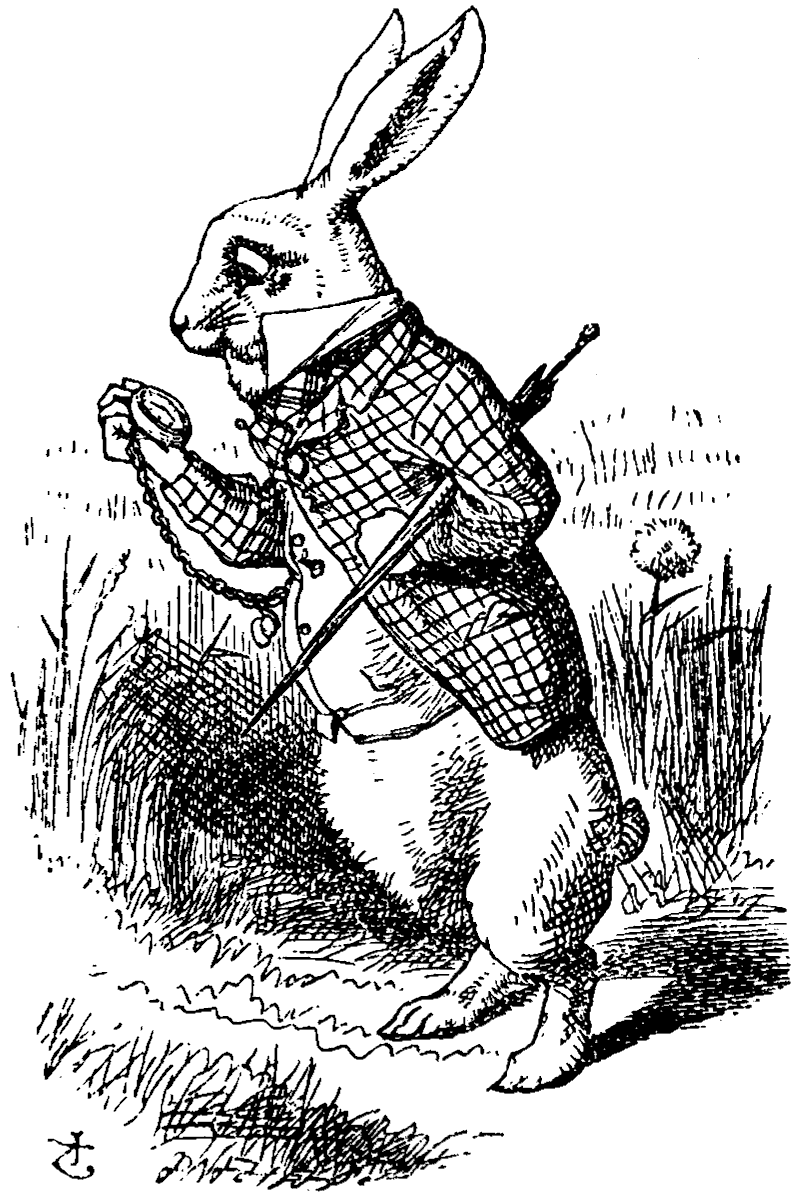
\includegraphics[width=4cm]{rabbit}\\
\vspace{0.5cm}
\vfill
{written with love by:\par}
\vspace{0.8cm}
%\large
\heartpar{Ettore Mariotti, Andrea Pittaro, Enrico Lovisotto, Davide Peron, Federico Mason, Lorenza Prospero, Cristina Gava, Matteo Ciprian}
\end{center}

\begin{center}
\noindent\makebox[\linewidth]{\rule{\textwidth}{0.4pt}}
\textsc{Academic Year 2016/2017}
\end{center}
\end{titlepage}
\begin{titlepage} %------------------------------ TITLE PAGE
\begin{center}

\hspace{0.5cm}
\vspace{-1.4cm}

\emph{\Huge{NETWORK MODELING}} \\
\textit{- Any Question? -}\\
\vspace{0.4cm}
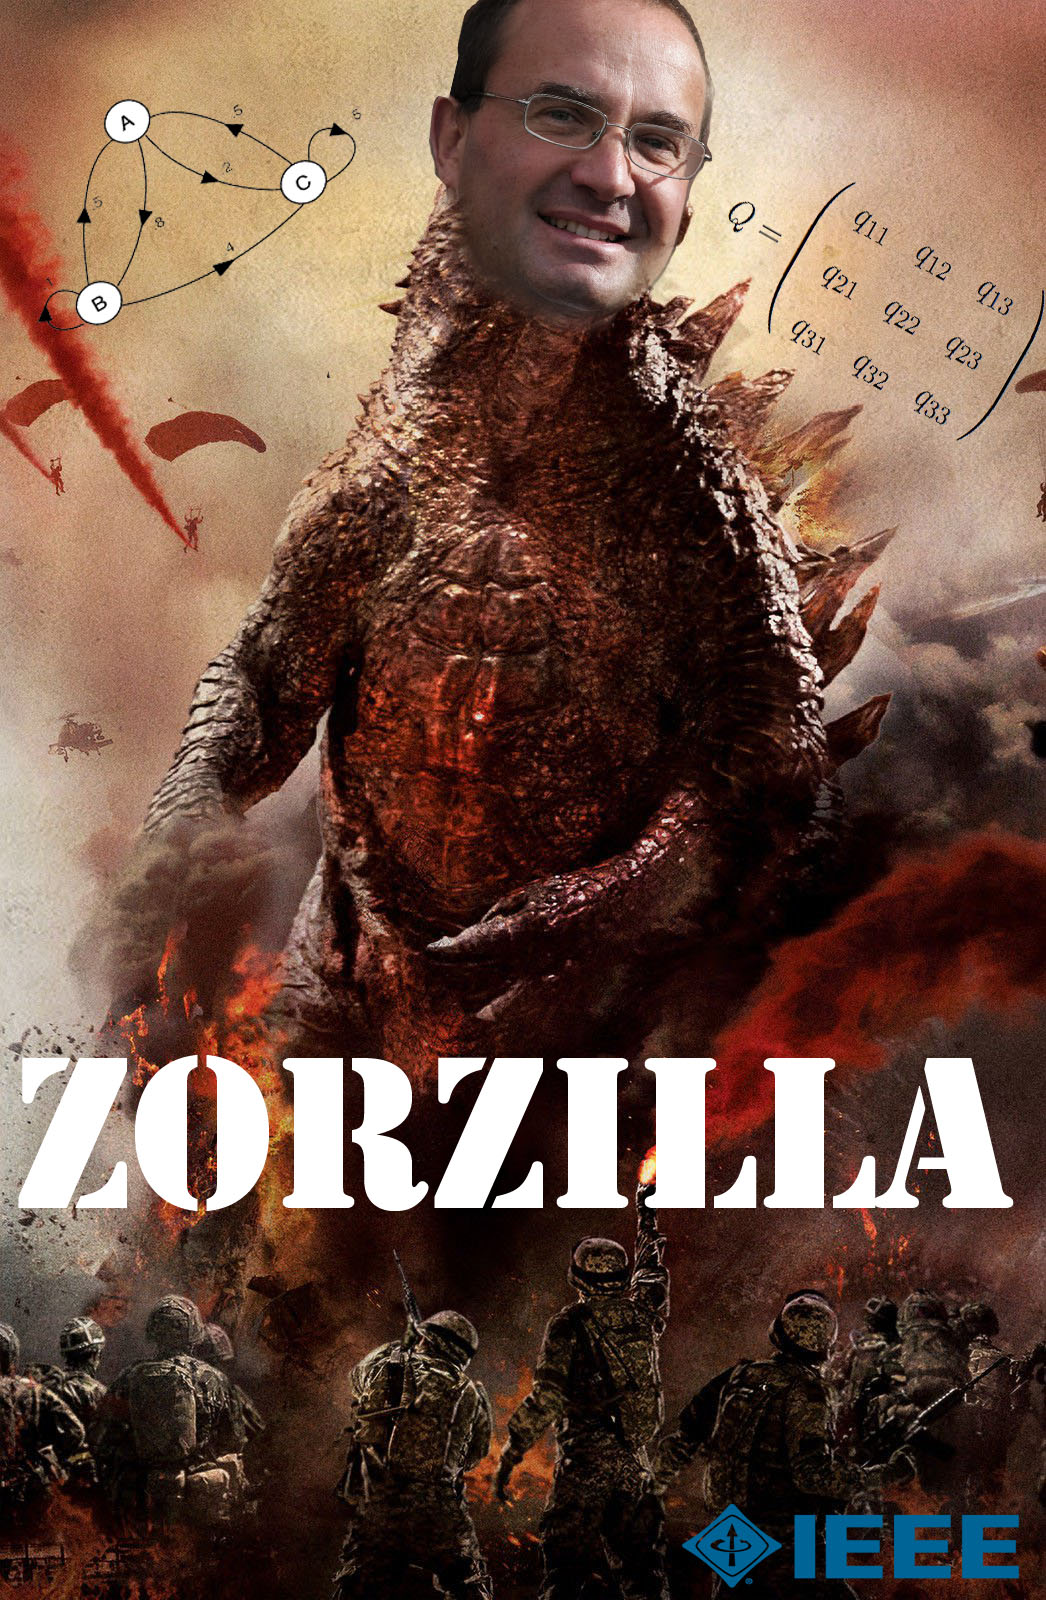
\includegraphics[width=10cm]{Zorzilla}\\
\vfill
{written with love by:\par}
\vspace{0.2cm}
%\large
\textbf{Ettore Mariotti, Andrea Pittaro, Enrico Lovisotto, Davide Peron, Federico Mason, Lorenza Prospero, Cristina Gava, Matteo Ciprian}
\end{center}
\vfill
\begin{center}
\noindent\makebox[\linewidth]{\rule{\textwidth}{0.4pt}}
\textsc{Academic Year 2016/2017}
\end{center}
\end{titlepage}

\begingroup %------------------------------ CONTENTS
  \makeatletter
  \renewcommand\thmt@listnumwidth{3em}
  \let\ps@plain\ps@empty
  \makeatother
  \tableofcontents
%theorem listing
  \listoftheorems[ignoreall,show={theorem}]
  \begingroup
    \let\clearpage\relax
    \listoftheorems[ignoreall,show={definition}]
  \endgroup
  \clearpage
\endgroup

\mainmatter
\chapter{Introduction}
\section{Topics of the course}
\begin{itemize}
  \item Review of probability theory
  \item Markov chains
  \item Poisson processes
  \item Example of applications protocols
  \item Random access protocols
\end{itemize}
\section{Review of probability theory}
Let $X_n, X_t$ be two different instances of a random variable (r.v.). We will use
\textit{t} as a subscript if the r.v. is continuous ($t \in \mathbb{R}$), \textit{n} if the r.v. is discrete ($ n \in \mathbb{Z}$)

Let \textit{A},\textit{B} be two events, then:
\begin{itemize}
  \item if $A \cap B = \emptyset$, then A and B are disjoint
  \item $P[A \cup B] = P[A]+P[B] - P[A \cap B]$
  \item $0\le P[A] \le 1$
  \item $P[A \cup B] \le P[A]+P[B]$
  \item $ P[\Omega]=1 $ and $P[\emptyset]=0$ with $\Omega$ the Universe set
\end{itemize}
\subsection{Total probability law}
Given $A_i \cap A_j = \emptyset \;\; \forall i \neq j $, then $\bigcup\limits_{i=1}^{+\infty} A_i \, = \Omega$.
Moreover $\mathbb{P}[B]=\sum\limits_{i=1}^{+\infty} \mathbb{P}[B \cap A_i]$.

If $\mathbb{P}[A \cap B] = \mathbb{P}[A]\cdot \mathbb{P}[B] \implies A,B$ \textit{are} \textbf{independent}.

\subsection{Distribution function (PMD)}\label{sec:pmd}
$F(x) = \mathbb{P}[X \le x]$ is called the distribution function and has the following properties:
\begin{enumerate}
  \item $\lim\limits_{x \to -\infty} F(x) = 0$ \quad and \quad $\lim\limits_{x \to +\infty} F(x) = 1$
  \item F is monothonic non-decreasing $\implies$ if $x_1 > x_2 \implies F(x_1)\ge F(x_2)$
  \item F(x) is continuous from the right
\end{enumerate}
We define $f(x)=F'(x)$ the probability density function \textit{PDF}.

\subsection{Moment}
We define  the moment as:
$\mathbb{E}[X^m]=
\begin{cases}
    \sum\limits_{i} {x{_i}^{m} \cdot \mathbb{P}[X=x_i]} & \text{if X is discrete } \\
    \int_{-\infty}^{+\infty} {x^{m} \cdot f(x) dx }  & \text{if X is continuous}
\end{cases}$
In particular if m=1, we obtain the mean, if m=2 we get the power (and in particular if $\mathbb{E}[X]=0$ we obtain the variance).\\
Defining $\mu = \mathbb{E}[X]$, we say that $\mathbb{E}[(X-\mu)^m]$ is the center moment.\\
We will denote $\mathbb{E}[g(x)]=\int_{-\infty}^{+\infty} g(x)\, d F_X(x)$

\subsection{Joint probability}
We define the joint probability of two variables as
\begin{equation*}
  $$F_{XY}(x,y)=\mathbb{P}[X\le x , Y \le y] \stackrel{\text{cont. case}}{=} \int_{-\infty}^{+\infty}\int_{-\infty}^{+\infty} f_{XY}(\eta,\xi) d\eta d\xi$$
\end{equation*}

From what we obtain in \ref{sec:pmd}, we can write \\
\begin{equation*}
  $$F_X(x)=F_{XY}(x,+\infty)=\lim\limits_{y \to +\infty} F_{XY}(x,y)$$
  $$F_Y(y)=F_{XY}(+\infty,y)=\lim\limits_{x \to +\infty} F_{XY}(x,y)$$
\end{equation*}
If X and Y are independent ($X \indep Y$), we have
\begin{itemize}
  \item $F_{XY}(x,y)=F_X(x)\cdot F_Y(y) \; \forall x,y$
  \item $cov(X,Y) = \mathbb{E}[(X - \mu_X)\cdot (Y - \mu_Y)] = \mathbb{E}[X \cdot Y]-\mu_X \cdot \mu_Y$
\end{itemize}
If X and Y are uncorrelated ($X \bot Y$) $\implies cov(X,Y)=0$.

\subsection{Conditional probability}
\begin{equation}
  $$\mathbb{P}[A | B]= \frac{\mathbb{P}[A \cap B]}{\mathbb{P}[B]} \; \text{with $\mathbb{P}[B]\ne 0$}$$ \\
  $$\implies \mathbb{P}[A \cap B ] = \mathbb{P}[A | B ]\cdot \mathbb{P}[B]$$
\end{equation}\\
From the total probability law we can write\\
$$\mathbb{P}[A]= \sum\limits_{i=0}^{+\infty}\mathbb{P}[A|B]\cdot \mathbb{P}[B_i]$$

Suppose we have $X \indep Y \text{ and } Z=X+Y$. Then $F_Z(z) = \mathbb{P}[Z\le z] = \mathbb{P}[X+Y \le z]$
Calculating F(z) can be more difficult with two variables. We will proceed this way:
\\
\begin{equation}
  $$
  \begin{split}
    E_{Y}[\mathbb{P}[X+Y \le z | Y]]  &\stackrel{\text{if X,Y are cont.}}{=} E_Y [\mathbb{P}[X \le Z - Y | Y]] = E_Y[F_X(z-Y)]\\
    &=\int_{-\infty}^{+\infty}F_x(z-y) \cdot dF_Y(y) \\
    &\implies f_Z(z) = F'_z(z) = \int_{-\infty}^{+\infty}{f_X(z-y)\cdot f_Y(y) dy} \\
    &=\int_{0}^{z}{f_X(z-y) \cdot f_Y(y) dy}
  \end{split}
  $$
\end{equation}


\subsection{Charateristic Function (C.F)}
(This can be found at KT pp 10-13)
\begin{equation}
  $$\phi(t) = \int_{-\infty}^{+\infty}e^{\imath \lambda t} dF(\lambda) = \mathbb{E}[e^{\imath t x}]\stackrel{\text{ x cont.}}{=}
  \int_{-\infty}^{+\infty}e^{\imath \lambda t} \cdot p(\lambda) d\lambda
  \\ \implies$$
\end{equation}
\begin{enumerate}
  \item $\phi(t)$ fully describes the statistics of X (the Fourier transform is a  one-to-one map )
  \item The characteristic function of the sum of independent variables is the product
  \item $\phi'(t)=\frac{d}{dt} \mathbb{E}[e^{\imath \cdot t \cdot x}]=\mathbb{E}[\imath \cdot x \cdot e^{\imath \cdot t \cdot x}]$ \\
  if t=0 $\implies \mathbb{E}[\imath \cdot x]=\imath \cdot \mathbb{E}[ X] = \phi'(0)$
  \item $\phi^{(k)}(0) = (\imath)^k \cdot \mathbb{E}[X^k] \implies \phi(t)$ is the \textbf{moment-generating function}
\end{enumerate}


For integer and non negative r.v. :
$$g(s)=\sum\limits_{k=0}^{+\infty}p_k \cdot s^k = \mathbb{E}[S^X]$$

$$\phi(t) = g(e^{\imath \cdot t})$$

Doing the derivative of g(s) we obtain:
\begin{equation}
   $$
  \begin{split}
    & g'(s) = \sum\limits_{k=0}^{+\infty} p_k \cdot k \cdot s^{k-1}
    \implies g'(1) = \sum\limits_{k=0}^{+\infty} k \cdot p_k \cdot = \mathbb{E}[X] \\
    & g''(s) = \sum\limits_{k=0}^{+\infty} p_k \cdot k \cdot (k-1) \cdot s^{k-2}
    \implies g''(1) = \sum\limits_{k=0}^{+\infty} k \cdot p_k = \mathbb{E}[X^2]-\mathbb{E}[X] \\
    &\implies \mathbb{E}[X^2] = g''(1)+g'(1) \; \; var(X) = g''(1)+g'(1)-(g'(1))^2
  \end{split}
  $$
\end{equation}

\subsection{Random Sum}
Now, let $X_1, X_2, \dotsc \; \text{ and }\; N \in \mathbb{N}$ a random number. Then $R=\sum\limits_{i=1}^{N}x_i$
is a random sum, because the sum is made of random $x_i$ random terms and $N$ is a random number.

\begin{equation}$$
  \begin{split}
    g_R(s)&=\mathbb{E}[s^R]=\mathbb{E}[s^{X_1+X_2+\dotsc+X_N}]=\sum\limits_{n=0}^{+\infty} \mathbb{P}[N=n]\cdot \mathbb{E}[s^{\sum_{i=0}^{n}X_i}|N=n]\\
    &=\sum\limits_{n=0}^{+\infty} \mathbb{P}[N=n]\cdot [g(s)]^n=g_N(g(s))
    \\ & \implies g_R(s) = g_N(g(s))
  \end{split}$$
\end{equation}
The mean and the variance of the moment generating functions can be calculated as follows:
\begin{equation}
$$
\begin{split}
  g'_R(s) &= g'_N(g(s)) \cdot g'_(s) \\
  g'_R(1) &= g_N'(1)\cdot g'(1) = \mathbb{E}[N]\cdot \mathbb{E}[X]=\mathbb{E}[R]\\
  &=\mathbb{E}[N^2-N]\cdot (\mathbb{E}[X])^2 + \mathbb{E}[N]\cdot \mathbb{E}[X^2-X] \\
  &=\mathbb{E}[N^2]\cdot \mathbb{E}[X]^2 - \mathbb{E}[N] \cdot \mathbb{E}[X]^2 +\mathbb{E}[N]\cdot \mathbb{E}[X^2] - \mathbb{E}[N]\cdot \mathbb{E}[X]\\
  & \implies var(R) = \mathbb{E}[R^2]-\mathbb{E}[R]^2 = g''_R(1)+g'_R(1)-[g'_R(1)]^2\\
  &=\mathbb{E}[N^2] \cdot \mathbb{E}[X]^2 + \mathbb{E}[N] \cdot var(X) - \mathbb{E}[N]\cdot \mathbb{E}[X] + \mathbb{E}[N] \cdot \mathbb{E}[X] - (\mathbb{E}[N] \cdot \mathbb{E}[X])^2 \\
  &= \mathbb{E}[X]^2 \cdot (\mathbb{E}[N^2]-\mathbb{E}[N]^2) + \mathbb{E}[N] \cdot var(X)
\end{split}
$$
\end{equation}

\textbf{So}
\begin{itemize}
  \item $\mathbb{E}[R] = \mathbb{E}[N] \cdot \mathbb{E}[X]$
  \item $var(R) = \mathbb{E}[N] \cdot var(X) + var(N) \cdot \mathbb{E}[X]^2$
\end{itemize}

What we saw just above is used in queueing systems when transmitting: queue length is N, random,
and the queue has packets of length X\textsubscript{i}.

\section{Distributions}
\subsection{Bernoulli}
Let $X \in \{0,1\}, \, p = \mathbb{P}[X=1]$, then $\mathbb{E}[X]=p, \, var(X)=p \cdot (1-p)$
We define $\chi(A)$ as the indicator function.

\subsection{Binomial}
Let $n$ be the number of i.i.d experiments with $\mathbb{P}[success]=p$. Let Y be the counter of the successes:
$Y=\sum\limits_{i=1}^{n} x_i$. We get $\mathbb{P}[Y=k]= \frac{n!}{k! \cdot (n-k)!}\cdot p^k \cdot (1-p)^{n-k}$

\subsection{Geometric}
Let Z be the counter of failure prior to the first success. We have $\mathbb{P}[Z=k] = p \cdot (1-p)^{k-1}$ with $k=0,1,\dots$, \\
We get $\mathbb{E}[Z]=\frac{1-p}{p} \; var(Z)=\frac{1-p}{p^2}$.
Sometimes books refer to $Z'=Z+1$ as the number of failure with the first success. In that case we have:\\
$\mathbb{E}[Z']=\frac{1}{p}; \quad var(Z')=\frac{1-p}{p^2}=var(Z)$

\subsection{Poisson}
Let $X$ be a Poisson r.v. with parameter $\lambda$. Then $\mathbb{P}[X=k] =  \frac{\lambda^k \cdot e^{-\lambda}}{k!}$ with $k=0,1,\dots$
\\
$\mathbb{E}[X]=\sum\limits_{k=0}^{+\infty}k \cdot \frac{\lambda^k \cdot e^{-\lambda}}{k!}= \lambda \sum\limits_{k=1}^{+\infty}\frac{\lambda^{k-1}\cdot e^{-\lambda}}{(k-1)!}=\lambda$
and $var(X)=\lambda$

Poisson r.v. play the role in the discrete as the gaussian in the continuos. There exists a theorem similar to CLT that states that under mild assumptions discrete r.v. converges to Poisson (will be better clarified with the Law of rare events).

\subsection{Exponential}
Let $T$ be an exponential r.v. in the form of
$$f_T(t)=
\begin{cases}
  \lambda \cdot e^{-\lambda \cdot t} & t \ge 0 \\
  0 & t <0
\end{cases}
$$
\\
Then $\mathbb{E}[X]= \frac{1}{\lambda}; \quad var(X)=\frac{1}{\lambda^2}$

The exponential is a r.v. good to model inter-arrival time and reliability (time in-between disasters)
What is the value of $\mathbb{P}[T-t > x | T>t]$?

\begin{equation}
  $$\mathbb{P}[T-t > x | T>t]=\frac{\mathbb{P}[T-t > x , T>t]}{\mathbb{P}[T>t]}=\frac{\mathbb{P}[T > t+x ]}{\mathbb{P}[T>t]}=\frac{1-\mathbb{P}[T \le t+x]}{1-\mathbb{P}[T\le t]}=\frac{e^{-\lambda \cdot (t+x)}}{e^{-\lambda \cdot t}} = e^{-\lambda \cdot x}$$
\end{equation}
We proved that the exponential r.v. is memoryless\footnote{If I observe that a the machine is working, it's like it's new. Not very realistic, but mathematically convenient.}

\subsection{Uniform}
$\mathbb{E}[\mathbb{U}]=\frac{a+b}{2},\quad var(\mathbb{U})=\frac{(b-a)^2}{12}$


\subsection{Gamma (also called Erlang distribution)}
Let $\alpha >0 , \lambda >0$. Then the PDF of a gamma-distributed r.v. is
\begin{equation}
  $$f(x) = \frac{\lambda}{\Gamma(\alpha)}\cdot (\lambda \cdot x)^{\alpha -1} \cdot e^{-\lambda \cdot x} \text{ with } x\ge 0$$
\end{equation}

For the expectation and the variance, we have: $$\mathbb{E}[G]=\frac{\alpha}{\lambda}, \qquad var(G)=\frac{\alpha}{\lambda^2}$$

Which is the same as $\alpha$ times $\mathbb{E}[exp]$ and $\alpha$ times $var(exp)$.
\\ If $\alpha \in \mathbb{N} \implies \Gamma(\alpha) = (\alpha-1)!$ and the gamma
distribution is the sum of $\alpha$ i.i.d exponential r.v. of parameter $\lambda$.

\begin{equation} $$
  \begin{split}
  \mathbb{E}[X]&\stackrel{discrete}{=} \sum\limits_{k=0}^{+\infty} k \cdot \mathbb{P}[X=k]
  \stackrel{\text{can be shown  that}}{=} \sum\limits_{k=0}^{+\infty} \mathbb{P}[X>k] \quad\mbox{  (beautiful)}\\
  &=0 \cdot p(0) + 1 \cdot p(1) + 2 \cdot p(2) + \dots \\
  &= p(1) + p(2) + p(3)+ \dots \qquad \mathbb{P}[X>0]\\
  & \qquad \qquad + p(2) + p(3) +\dots \quad \mathbb{P}[X>1]\\
  & \qquad \qquad \qquad \qquad + p(3)+ \dots \quad \mathbb{P}[X>2] \\
  & \dots
  \end{split}$$
\end{equation}
where $\mathbb{P}[X=k]=p(k)$ and $\mathbb{P}[X>k]$ is the complementary distribution

In the continuous case
\begin{equation}$$
  \begin{split}
    \mathbb{E}[X] &= \int_{0}^{+\infty} 1-F(x) dx = \int_{0}^{+\infty} x \cdot f(x) dx
    &=\int_{0}^{+\infty} e^{-\lambda \cdot x} dx = \frac{1}{\lambda}
  \end{split}$$
\end{equation}

\section{Conditional Distribution}
(Note: this material can be found in Chapter 2 K. T.).\\
We saw the Total Probability theorem and how to use it to find a probability with subsetting.\\
Let's now extend it to the composite PMD. Let $X,Y$ be two indipendent r.v, with $\mathbb{P}[Y=y]\neq 0$.
Then, $\forall x,y$
\begin{equation}$$
  \begin{split}
    \mathbb{P}[X\le x, Y \le y] &= \sum \limits_{\eta \le y} \mathbb{P}[X \le x , Y \le \eta] \\
    &\stackrel{discrete}{=} \sum \limits_{\eta \le y} F_{X|Y}(x | \eta) \cdot \mathbb{P}[Y=\eta]\\
    &\stackrel{continuous}{=} \int_{\eta \le y} F_{X|Y}(x|\eta) dF_Y(\eta)
  \end{split}$$
\end{equation}
We can try to find the expectation of $g(x)$ which is a function of Y using the conditioning. So we obtain:
\begin{equation}
  $$\mathbb{E}[g(x)]=\mathbb{E}[\mathbb{E}[g(x)|Y]] = \int_{-\infty}^{+\infty}\mathbb{E}[g(x)|Y=\eta] dF_Y(\eta)$$
\end{equation}

\textbf{SO}
\begin{equation}
  \begin{split}
   &\forall x,y \\
  &\mathbb{P}[X\le x , Y \le y] = \int_{\eta \le y} F_{X|Y}(x|\eta) dF_Y(\eta)\\
  &\forall x \quad \mathbb{P}[X \le x] = \int_{-\infty}^{+\infty}F_{X|Y}(x|\eta) dF_Y(\eta) \\
  &\mathbb{E}[g(x)]=\int_{-\infty}^{+\infty}
  \mathbb{E}[g(x)|Y=\eta] dF_Y(\eta)
  \end{split}
\end{equation}

\subsection{Example binomial}
EMPTY

\subsubsection{Transform approach}
\begin{equation}
  \begin{split}
  g_N(s)=\sum \limits_{n=1}^{+\infty} \beta \cdot (1-\beta)^{n-1}\cdot s^n = \frac{\beta \cdot s}{1-(1-\beta)\cdot s}\\
  \phi_T=\mathbb{E}[e^{\jmath \cdot t \cdot x}] = \int_{0}^{+\infty} e^{\jmath \cdot t \cdot x} \cdot \lambda \cdot e^{ \lambda \cdot x} dx = \frac{\lambda}{\lambda - \jmath \cdot t} \\
  \phi_Z = g_N(\phi_T(t))=\frac{\beta \cdot \frac{\lambda}{\lambda - \jmath \cdot t}}{1-(1-\beta)\cdot \frac{\lambda}{\lambda - \jmath \cdot t}} =
   \frac{\beta \cdot \lambda}{\lambda - \jmath \cdot t -\lambda - \beta \cdot \lambda} = \frac{\beta \cdot \lambda}{\beta \cdot \lambda - \jmath \cdot t}
  \end{split}
\end{equation}
In the last row we can see how the the composition changed only the parameter: $\lambda$ becomes $\beta \cdot \lambda$.

We recall that $f_{X|Y} = \frac{f_{XY}(x,y)}{f_Y(y)}$ with $f_Y(y)\neq 0$ in the considered interval.
We can then derive
\begin{equation}
  \begin{split}
  F_{X|Y}(x|y) = \int_{-\infty}^{x}f_{X|Y}(\xi,y)d\xi\\
  \forall x,y \quad \mathbb{P}[X \le x , Y \le y] &= \int_{-\infty}^{x}d\xi \int_{-\infty}^{y}f_{XY}(\xi,\eta) d\eta\\
  &=\int_{-\infty}^{y}f_Y(\eta) \int_{-\infty}^{x}f_{X|Y}(\xi,\eta) d\xi d\eta \\
  =&\int_{-\infty}^{y}F_{X|Y}(x,\eta) dF_Y(\eta)
  \mathbb{E}[g(x)] &= \int_{-\infty}^{+\infty} \int_{-\infty}^{+\infty}g(\eta) f_{XY}(\xi,\eta) d\eta  d\xi \\
  &= \int_{-\infty}^{+\infty} f_Y(\eta) \int_{-\infty}^{+\infty}g(\eta) f_{X|Y}(\xi,\eta)   d\xi d\eta \\
  &= \int_{-\infty}^{+\infty}\mathbb{E}[g(x)|Y=\eta] dF_Y(\eta)
  \end{split}
\end{equation}

\chapter{Markov Chains}

\section{Introduction}
A markov process is a process $X_n \text{ or } X_t$ s.t.
\begin{equation}
	\prob[X_{n+1} = j | X_0 = i_0, X_1 = i_1, \dots, X_n = i_n] = \prob[X_{n+1} = j | X_n=i_n] = P
\end{equation}

with P as the \textit{one-step probability}. From now on, the notation for that probability will be $P_{i,j}^{n,n+1}=P_{i,j} \quad \forall n$ if the MC is homogeneous, i.e. the transition probabilities are stationary.

We can suppose $n\ge 0$ and we'll have the \textbf{transition probability matrix}, which will characterize the process as
\begin{equation} \bm P=\begin{pmatrix}
	P_{00} & P_{01} & \cdots  \\
	P_{10} & P_{11} & \cdots \\
	\vdots & \vdots & \ddots  \\
 	\end{pmatrix}
	\text{with } P_{i,j}\ge 0 \forall i,j \quad \text{ and } \sum\limits_{j=0}^{+\infty}P_{i,j} = 1 \quad \forall i
\end{equation}

For example
\begin{equation}
	\prob[X_3 = i_3 , X_2 = i_2, X_1 = i_1, X_0 = i_0]=P_{i_0}\cdot P_{i_0,i_1}\cdot P_{i_1,i_2}\cdot P_{i_2,i_3}
\end{equation}

The description of a markov process is given from the initial state probability and the transition probability matrix.

\section{Stability of a process}
Suppose a system where customers arrive independently and are queued in the system before getting served.
Suppose the service time occupies only one slot and all the slots for service time have same duration.
If the queue is empty, that time slot is wasted.
Now let the number of users arriving in the n-th slot be $\xi_n$ and the number of users in
the system in the n-th slot  be $X_n$. Then we have:
 \begin{equation}
 	\begin{split}
 	&\prob[\xi_n=k] = a_k \text{, probability of k arriving users at time n}\\
  	&X_{n+1}=
		\begin{cases}
 			X_n -1 +\xi_n &  \text{if } X_n >0 \\
 			\xi_n 			 	&  \text{if } X_n = 0
 		\end{cases}
 	\end{split}
 \end{equation}

The transition probability matrix:
\begin{equation} \bm P=\begin{pmatrix}
	a_{0} & a_{1} & a_2 & \cdots  \\
	a_{0} & a_{1} & a_2 & \cdots  \\
	0			& a_{0} & a_{1} & \cdots  \\
	0 		& 0			& a_{0} & \cdots  \\
	\vdots & \vdots & \vdots & \ddots &  \\
\end{pmatrix}
\end{equation}
\begin{definition}[Behavior of a MC]
Let $\rho=\sum\limits_{k=0}^{+\infty} k \cdot a_k$. We say that for
\begin{equation} \rho : \begin{cases}
	>1 & \text{\textbf{unstable }: the system will never be able to serve everybody}\\
	=1 & \text{\textbf{unstable \textit{unless deterministic}}: sooner or later the system will fail}\\
	<1 & \text{\textbf{stable}: the queue tends to be empty}
\end{cases}\end{equation}
\end{definition}

\section{First step analysis}
\begin{definition}[Absorbent state]
	 A state $i$ is defined $absorbient$ if it is valid the following condition:$p_{ij}=0$ $\forall j\neq i$ and $p_{ii}=1$. In practice, when a chain incur in the state $i$ no transition to other different states is longer possible. Therefore  the chain will remain "absorbed" in it. 
\end{definition}
\begin{definition}[Absorbent time]
	Being $A$ the set of the absorbent states of a particular markov chain, the absorbent time is defined in the following way: 
	\begin{equation}
	T= \min \{n\geq0: X_n \in A \}
	\end{equation}
\end{definition}
"First step analysis" is a "standard procedure" applied to resolve some particular Markov Chain in which there is one of more absorbent state.
 We are interested in computing two fundamental quantities:
\begin{itemize}
	\item The probability of absorption given a starting point $i$ :  $ u_i=P[X_T\in A | X_0=i ]$
	\item The expected absorption time given a starting point $i$ : $v_i= E[T|X_0=i]$
\end{itemize}
\subsection{First Step Analysis: General Method}
\begin{itemize}
	\item Reorganize the markov chain according to the following rules
	\begin{itemize}
		\item The states from $0,..r-1$ transient;
		\item The states from $r,...,N$ absorbent.
	\end{itemize}

	\item  Reorganize the transition matrix according to the following rules :
     \begin{equation} P=\begin{pmatrix}
     P_{00} & P_{01} & \cdots & P_{0r}& P_{0(r+1)} &\cdots & \cdots &P_{0N} \\
     P_{00} & P_{01} & \cdots & P_{1r}& P_{1(r+1)}& \cdots & \cdots & P_{1N}\\
     \vdots & \vdots & \ddots  \\
     P_{r0}=0 & P_{r1}=0& \cdots &P_{rr}=1& 0 & \cdots & \cdots &0\\
     P_{(r+1)0}=0 & P_{(r+1)1}=0& \cdots &P_{(r+1)r}=0& P_{(r+1)(r+1)}=1& 0&  \cdots&  0\\
     \vdots & \vdots & \ddots  \\
     P_{N0}=0 & P_{N1}=0& \cdots &P_{Nr}=0& P_{N(r+1)}=0& 0&  \cdots&  P_{NN}=1\\
     
     \end{pmatrix}
$$   
     \end{equation}
     As shown in the figure above the matrix is composed by three parts:
     \begin{itemize}
     	\item In the upper part there are the transitions probability from the not-absorbient states.
     	\item In the low left corner there are the transition probability from  the absorbent states to the not-absorbent states: these can be have only 0 for the definition of absorbent state.
     	\item In the low-right corner there are the transition probabilities from  the absorbent states to the absorbent states. This is a $(N-r)$ x$(N-r)$ identity submatrix: once a chain enters in one absorbent state, it can only remain in it and cannot go away 
     	
     \end{itemize} 
    \item In order to compute the the probability of absorption given a starting point $i$ it is possible to write the following:
    \begin{equation} 
    \begin{split}
      u_{ik} = P[X_T=k|X_0=i]= \sum\limits_{j=0}^N u_{jk}P_{ij}=\\
      \sum\limits_{j=0}^N P[X_T=k|X_0=i,X_1=j]P[X_1=j|X_0=i]=\\
      = P_{ik}+\sum\limits_{j=0}^N 0*P_{ij} +\sum\limits_{j=0}^{r-1} u_{jk}P_{ij},
      \\
      P_{ik}+\sum\limits_{j=0}^{r-1} u_{jk}P_{ij}              
      \end{split}      
     \end{equation}
     
       this is valid for $i= 0,1,..r-1$
    Intuitively the probability of being absorbed in a state $k$ starting in $i$ is equal to the transient probability of the transition $i\rightarrow k$ plus the probabilities of being absorbent from another not-absorbent state ($j \in (0,...r-1)$) weighted by the probability of doing the transition  $i\rightarrow j$ ($P_{ij}$). 
    In this case the unknown values are the $u_{jk}$ thus 
    a system of $ r-1$ has to be solved in order to compute properly $u_{ik}$ probability.
     \newline Trivially for $i= r,.. , N$, $u_{ik}=0$ for $i\neq k$ and $u_{ik}=1$ $i=k$.
 
 \item In order to compute the expected absorption time given a starting point $i$ : $v_i= E[T|X_0=i]$ a very similar method is applied: 
 \begin{equation}
 v_i= 1 + \sum\limits_{j=0}^{r-1} P_{ij} v_j
  \end{equation}
   Intuitively the expected absorption time from i is equal to 1 with probability 1 (at least one transition has to be done) plus the  the expected absorption time starting from j weighted by the probability of doing the transition  $i\rightarrow j$ ($P_{ij}$) where j (of course) is a not-absorbent state.
   
  \item Remember that all the equations written above are recursive because they will have the following form :
  \begin{equation}
     u_{ik}= P_{ik}+\sum\limits_{j=0}^{r-1} u_{jk}P_{ij} =  P_{ik}+ u_{0k}P_{i0} + .... + u_{ik}P_{ii} + ... +  u_{(r-1)k}P_{i(r-1)}
   \end{equation}  
\end{itemize}

%\subsection{First passage time}
%Another application of first step analysis is the computation of so-called "First-passage-time" define in the following way:
%	\newline
%	$\theta_{ij}$= \# of transitions to reach j starting from i 
%% TO BE DONE ... 
\section{Random walk}
\begin{figure}[h]
	% \documentclass{standalone}
%
% \usepackage{tikz}
% \usetikzlibrary{automata,positioning}
%\begin{document}
\begin{tikzpicture}
  \node[state] at (-10,0) (0) {0};
  \node[state] at (-8,0)  (1) {1};
  \node[state] at (-6,0)  (2) {2};
  \node[state] at (-4,0)  (3) {3};
  \node[] at (-2,0 )  (infty) {$\dots$};

  \draw[every loop, auto=right, >=latex]
      (1) edge[bend right, auto=left]  node[above] {$q_1$} (0)
      (0) edge[bend right, auto=right] node {$p_0$} (1)
      (1) edge[loop above]             node {} (1)
      (0) edge[loop above]             node {} (0)
      (2) edge[bend right, auto=left]  node[above] {$q_2$} (1)
      (1) edge[bend right, auto=right] node {$p_1$} (2)
      (2) edge[loop above]             node {} (2)
      (1) edge[loop above]             node {} (1)
      (3) edge[bend right, auto=left]  node[above] {$q_3$} (2)
      (2) edge[bend right, auto=right] node {$p_2$} (3)
      (3) edge[loop above]             node {} (3)
      (2) edge[loop above]             node {} (2)
      (infty) edge[bend right, auto=left]  node {} (3)
      (3) edge[bend right, auto=right] node {} (infty);
\end{tikzpicture}
% \end{document}

	\caption{An infinite random walk MC. With relation to gambling, the MC rapresents the case
	where (1) the adversary has an infinite wealth (e.g.: casino), (2) the gambler can loose nothing in one game
	(3) all games have different probability to win or loose (4) the player can always recover }
	\label{}
\end{figure}
The theory around the random walks was developed to understand better the probability around the
gambling world using the MC theory. We now make some assumptions before starting the analysis on this topic.
\subsection{Assumptions:}
\begin{enumerate}
	\item The MC has \textbf{N+1} states, representing the status of the gambler' health.
	 Let 0 be the \textit{ruined gambler} state and N be the gambler' success;
	\item The gambler must always play;
	\item All the games are equal with
	\begin{description}
		\item[p] probability to go to an upper state by winning a game
		\item[q] probability to lose the game and go to a lower state
	\end{description}
\end{enumerate}
\begin{figure}[h]
	% \documentclass{standalone}
%
% \usepackage{tikz}
% \usetikzlibrary{automata,positioning}
% \begin{document}
\begin{tikzpicture}
  \node[state] at (-10,0) (0) {0};
  \node[state] at (-8,0)  (1) {1};
  \node[state] at (-6,0)  (2) {2};
  \node[state] at (-4,0)  (3) {3};
  \node[] at (-2,0 )  (infty) {$\dots$};
  \node[state] at (0,0)  (4) {$N-1$};
  \node[state] at (2,0)  (5) {$N$};

  \draw[every loop, auto=right, >=latex]
      (1) edge[bend right, auto=left]  node[above] {$q$} (0)
      (0) edge[bend right, auto=right] node {$p$} (1)
      (0) edge[loop above]             node {1} (0)
      (2) edge[bend right, auto=left]  node[above] {$q$} (1)
      (1) edge[bend right, auto=right] node {$p$} (2)
      (3) edge[bend right, auto=left]  node[above] {$q$} (2)
      (2) edge[bend right, auto=right] node {$p$} (3)
      (infty) edge[bend right, auto=left]  node[above] {$q$} (3)
      (3) edge[bend right, auto=right] node {$p$} (infty)
      (4) edge[bend right, auto=left]  node[above] {$q$} (infty)
      (infty) edge[bend right, auto=right] node {$p$} (4)
      (5) edge[bend right, auto=left]  node[above] {$q$} (4)
      (4) edge[bend right, auto=right] node {$p$} (5)
      (5) edge[loop above]             node {1} (5);
\end{tikzpicture}
% \end{document}

	\caption{Under the assumption given before, the MC can be represented as this picture}
	\label{}
\end{figure}

Let now define the probability that the gambler goes to ruin if he starts in state k
\begin{equation}\begin{split}
	u_k &= \prob[\text{gambler's ruin}|\text{initial wealth}=k] \\
	&=p \cdot u_{k+1} + q \cdot u_{k-1} \quad \text{with }k=1, \dots, N-1 \\
	u_0 &= 1 \quad u_N = 0
\end{split}\label{eq:defUk}
\end{equation}
We can now define the transition probability as follows

\begin{equation}\begin{split}
q \cdot \underbrace{(u_k - u_k-1)}{X_k} &= p \cdot \underbrace{\left(u_{k+1} -u_k\right)}{X_{k+1}} \\
X_{k+1} = \frac{q}{p}\cdot X_k \quad & X_{2} = \frac{q}{p}\cdot X_1 \quad X_{3} = \left(\frac{q}{p}\right)^2 \cdot X_1\\
\implies & X_{k} = \left(\frac{q}{p}\right)^{k-1}\cdot X_1
\end{split}\end{equation}
Let's now see what's the expression for $u_k$.
\begin{equation}\begin{split}
	\sum\limits_{i=1}^{k}X_i &= X_1 \cdot \sum\limits_{i=1}^{k}\left(\frac{q}{p}\right)^{i-1} \\
	\sum\limits_{i=1}^{k}X_i &= \sum\limits_{i=1}^{k}(u_i-u_{i-1}) = u_k - u_0 = u_k -1
	\implies & u_k = 1+ \sum\limits_{i=1}^k X_i
\end{split}\end{equation}
Now recalling eq. \eqref{eq:defUk}, we have that
\begin{equation}\begin{split}
	X_1 &= -\frac{1}{\sum\limits_{i=1}^N \left(\frac{q}{p}\right)^{i-1}}\\
	u_k &= 1- \frac{\sum\limits_{i=1}^k\left(\frac{q}{p}\right)^{i-1}}{\sum\limits_{i=1}^N\left(\frac{q}{p}\right)^{i-1}}
\end{split}\end{equation}
The $u_k$ result we obtained, includes also the extremal cases where k=0 and k=N.\\
If now we calculate the sum, we obtain
\begin{equation}
	u_k = 1- \frac{\frac{1-\left(\frac{q}{p}\right)^k}{1-\frac{q}{p}}}{\frac{1-\left(\frac{q}{p}\right)^N}{1-\frac{q}{p}}}=
	1-\frac{1-\left(\frac{q}{p}\right)^k}{1-\left(\frac{q}{p}\right)^N}
\end{equation}
We can now make two distinction cases using the Taylor approximation
\begin{equation}u_k=\begin{cases}
	1-\frac{1-\left(\frac{q}{p}\right)^k}{1-\left(\frac{q}{p}\right)^N} & p \neq q \\
	1-\frac{k}{N} & p=q
\end{cases}\end{equation}
Suppose now that the adversary has an infinity wealth, like a casino. The probability
that the gambler goes in ruin is
\begin{equation}
	\lim_{N \to +\infty} u_k =
	\begin{cases}
		1 & p<k \\
		\left(\frac{q}{p}\right)^k & p>q\\
		1 & p=q
\end{cases}\end{equation}
The last case may seem strange, but even if the game is fair ($p=q=\frac{1}{2}$), in an infinite time
a series of unfortunate events may occour and the gambler will reach $X_0$, his ruin.

\section{First passage time}
\begin{definition}[$\theta_{i,j}$]
We define $\theta_{i,j}$ to be the number of transitions to reach j from i for the first time.
\end{definition}
We now would like to know $\prob[\theta_{i,j}=n]$ and $\exp[\theta_{i,j}]$.

Let's start with the probability:
\begin{definition}
	We define the probability of going from state $i$ to state $j$ in $n$ steps, $\prob[\theta_{i,j}=n]$, as follows:
	\begin{equation}\begin{split}
		\prob[\theta_{i,j}=n] &= f_{i,j}(n)=\prob[X_n=j,X_m \neq j | X_0 = i] \quad \text{with m=1 \dots n-1}\\
		f_{i,j}(0)&=0 \quad \forall i,j \,\, \text{ because $n \ge 1$}\\
		f_{i,j}(0)&=P_{i,j} \cdot \delta(n-1) + \sum\limits_{k \neq j} P_{i,k} \cdot f_{k,j}(n-1)\\
	\end{split}\end{equation}
\end{definition}
\subsubsection{Example for a 2-state MC}
\begin{figure}
	\centering
  \begin{tikzpicture}
    [
      my circle/.style={minimum width=10mm, circle, draw},
      my label/.style={above=10pt, anchor=mid}
    ]
    \node[my circle] (1) at (-1,0) {$0$};
    \node[my circle] (2) at ( 1,0) {$1$};
    %\path [postaction={draw, {>[sep=5pt,reversed]}-{<[sep=5pt]}}, draw] (1) -- (2) node [very near start, my label] {$a$}  node [very near end, my label] {$\beta$} ;
		\path[->,draw] (1.south east)  edge[bend right=90] node [below] {$b$} (2.south west);
		\path[->,draw] (1.north east)  edge[bend left=90] node [above]  {$a$} (2.north west);
		\path [-stealth, draw] (2.south east) arc (-135:135:5mm) node [near end, my label] {$1-b$};
    \path [-stealth, draw] (1.south west) arc (-45:-315:5mm) node [near end, my label] {$1-a$};
  \end{tikzpicture}
	\caption{A two-state Markov chain}
	\label{fig:2sMC}
\end{figure}
For a two state \gls{mc} like the one in \ref{fig:2sMC}, we can write:
\begin{equation}\begin{split}
	f_{01}(n)&= P_{01} \cdot \delta(n-1) + P_{00} \cdot f_{01}(n-1) = a \cdot \delta(n-1) + (1-a)\cdot f_{01}(n-1)\\
	f_{01}(1)&=a \quad f_{01}(2)=a \cdot(1-a) \quad \dots \quad f_{01}(n) = a\cdot(1-a)^{n-1} n \ge 1 \\
	f_{11}(n) &= P_{11}\cdot \delta(n-1) + P_{10} \cdot f_{01}(n-1) =
	\begin{cases}
		1-b & n=1 \\ (1-a)^{n-2}\cdot a \cdot b & n>1
	\end{cases}
\end{split}\end{equation}

For a general \gls{mc}, we have
\begin{equation}\begin{split}
	P^{(n)} &= P^n \\
	P_{i,j}^{(n)} &= \sum\limits_{m=1}^n f_{i,j}(m) \cdot P_{j,j}^{(n-m)} \quad n \ge 1 \\
	f_{i,j}(n)&=
	\begin{cases}
		P_{i,j}^{(n)} -\sum\limits_{m=1}^{n-1} f_{i,j}(m) \cdot P_{j,j}^{(n-m)} & n \ge 2 \\
		P_{i,j}^{(n)} = P_{i,j} & n =1 \\
		0 & n=0
	\end{cases} \\
	\theta_{i,j}(n)&=
	\begin{cases}
		1 & \text{w.p. } P_{i,j} \\
		1+\theta_{k,j} &  \text{w.p. } P_{i,j} \text{ with } k \neq j
	\end{cases} \\
\end{split}\end{equation}

Let's now focus on the expectation of $\theta_{i,j}$. We can write:
\begin{equation}\begin{split}
	\exp[\theta_{i,j}] &= P_{i,j} + \sum\limits_{k \neq j} (1+\exp[\theta_{k,j}])\cdot P_{i,k}\\
	&\stackrel{(1)}{=} 1+ \sum\limits_{k \neq j} \exp[\theta_{k,j}] \cdot P_{i,k} \forall i \neq j\\
\end{split}\end{equation}
with \textit{(1)} $P_{i,j} + \sum\limits_{k\neq j}P_{i,k} =\sum\limits_{\forall k}P_{i,k} = 1 $
\\
We then get $N$ equations in $N$ unknowns, so the system can be solved.
\\
Now, with the example of the two state MC, we will show that the average return
time is the inverse of the in-state remaining probability.
\begin{equation}\begin{split}
	\exp[\theta_{0,1}] &= 1 + P_{00} \cdot \exp[\theta_{0,1}] \quad \exp[\theta_{0,1}] = \frac{1}{1-P_{00}} = \frac{1}{a}\\
	\exp[\theta_{1,0}] &= 1 + P_{11} \cdot \exp[\theta_{1,0}] \quad \exp[\theta_{1,0}] = \frac{1}{1-P_{11}} = \frac{1}{b}\\
	\exp[\theta_{0,0}] &= 1 + P_{01} \cdot \exp[\theta_{1,0}] =1+\frac{a}{b} = \frac{1}{1-P_{00}} = \left(\frac{b}{a+b}\right)^{-1}\\
	\exp[\theta_{1,1}] &= 1 + P_{10} \cdot \exp[\theta_{0,1}] =1+\frac{b}{a} = \frac{1}{1-P_{00}} = \left(\frac{a}{a+b}\right)^{-1}\\
	\lim_{n \to +\infty} P^n &=
	\begin{pmatrix}
		\frac{b}{a+b} & \frac{a}{a+b} \\
		\frac{b}{a+b} & \frac{a}{a+b}
	\end{pmatrix}
\end{split}\end{equation}

Analyzing the second order momentum, we have
\begin{equation}\begin{split}
	\exp[\theta_{i,j}^2] &= P_{i,j} + \sum\limits_{k \neq j} \exp[(1+\theta_{k,j})]\cdot P_{i,k}\\
	&= 1 + 2 \underbrace{\cdot \sum\limits_{k \neq j} \exp[\theta_{k,j}]\cdot P_{i,k}}_{\exp[\theta_{i,j}-1]} + \sum\limits_{k \neq j} \exp[\theta_{k,j}^2] \cdot P_{i,k}\\
	&= 2 \cdot \exp[\theta_{i,j}]-1 +  \sum\limits_{k \neq j} \exp[\theta_{k,j}^2] \cdot P_{i,k} \forall i \neq j \\
\end{split}\end{equation}

Which means that for the two-state MC, we have
\begin{equation} \begin{split}
	\exp[\theta_{01}^2] &= \frac{2 \cdot \exp[\theta_{01}]}{1-P_{00}} = \frac{\frac{2}{a}-1}{a} = \frac{2}{a^2} - \frac{1}{a}\\
	var[\theta_{01}] &= \frac{1-a}{a^2} \quad \text{same variance as a geometric r.v.} \\
	var[\theta_{10}] &= \frac{1-b}{b^2}\\
	\exp[\theta_{00}^2] &= 2 \cdot \exp[\theta_{00}]  -1 - P_{01}\cdot \exp[\theta_{10}^2] = 1 + \frac{a}{b} + \frac{2a}{b^2} \\
	var[\theta_{00}] &= \frac{a \cdot(2-a-b)}{b^2}\\
	var[\theta_{11}] &= \frac{b\cdot(2-a-b)}{a^2}\\
\end{split}\end{equation}

\subsection{Techniques to set up P matrix}
In this part, we will show some tips to set the P matrix, so that the solving and the product
will be easier when analyzing absorption time. First of all, you should discriminate
transient state and the one that creates the absorbing states, like the following:
\begin{equation} \begin{split}
	P&=\raisebox{-1\baselineskip}{\begin{blockarray}{cc}
      \begin{block}{(cc)}
          Q  & R \\
          0  & I \\
      \end{block}
			\parbox[c]{1.7cm}{\small 0,1,\dots,r-1 \text{transient}} & \parbox[c]{1.7cm}{\small r,\dots,n \text{absorbing}}
    \end{blockarray}}
	P^2 &= P \cdot P = \begin{pmatrix}
	Q^2 & Q \cdot R + R \\
	0 & I
	\end{pmatrix}	\\
\end{split}\end{equation}
which means that for the general case we have:
\begin{equation} \begin{split}
	P^n &= \begin{pmatrix}
	Q^n & \sum\limits_{i=0}^{n-1}Q^i \cdot R \\
	0 & I
	\end{pmatrix}
\end{split}\end{equation}
Let's now define $W_{i,j}^{(n)}$ as follows
\begin{definition}
	\begin{equation}
		W_{i,j}^{(n)} = \exp[\sum\limits_{l=0}^n \Chi \{ X_l=j\}|X_0=i] = \sum\limits_{l=0}^n\exp[\Chi \{ X_l=j\}|X_0=i]\sum\limits_{l=0}^n P_{i,j}^{(l)}
	\end{equation}
\end{definition}
Now suppose that $i,j$ are transient and put $W_{i,j}^{(n)}$ as element of a matrix. The resulting matrix will be:
\begin{equation}\begin{split}
	W^{(n)} &= I + Q + \dots + Q^n = I + Q \cdot W^{(n-1)} \\
	W &= \lim_{n \to +\infty} W^{(n)} = \sum\limits_{l=0}^{+\infty} [I-Q]^{-1} \cdot \vec{1}
\end{split}\end{equation}
If we sum, for all j transient states $W_{i,j}$  we obtain:
\begin{equation}
	\sum\limits_{j=0}^{r-1}W_{i,j} = \exp[\sum\limits_{n=0}^{T-1}\sum\limits_{j=0}^{r-1}\Chi\{X_n=j\}|X_0=i] = \exp[T|X_0=i]=v_i
\end{equation}
Let's now find the probability to go from a transient state ($i$) to an absorbing one($k$)
\begin{equation}
	U_{i,k}^{(n)} = \prob[T \le n , X_T = k | X_0=i] = \prob[X_n=k|X_0=i]=P_{i,k}^{(n)}
\end{equation}
This means that:
\begin{enumerate}
	\item $U^{(n)} = W^{(n-1)}\cdot R$
	\item $U=\lim_{n\to +\infty} U^{(n)} = W \cdot R = [I-Q]^{-1}\cdot R$
	\item $\tilde{P}=\begin{matrix} Q & r \\ \vec{0}&1 \end{matrix}$
\end{enumerate}
In conclusion, we found that the average first passage time is equal to the average
 absorption time, which is $[I-Q]^{-1}\cdot \vec{1}$
\section{Long Run Behaviour}
\subsection{Steady-state probabilities}

	\begin{definition}[Regular \gls{mc}]
		A regular \gls{mc} is a \gls{mc} with the following property:

		\begin{equation} \lim_{n \to \infty} P_{ij}^{(n)} = \lim_{ n \to \infty} Prob[ X_n=j | X_0 =i] = \pi_j > 0 \quad \forall i, j \end{equation}

	\end{definition}

	This tell us that:
	\begin{enumerate}
		\item Limit \textbf{exists} (not obvious)
		\item Limit is indipendent of the initial state
		\item Limit is \textbf{strictly} positive
	\end{enumerate}

	\begin{theorem}
		For a regular \gls{mc} with states 0, 1, ..., N the limit distribution $\bm\pi = (\pi_0,\pi_1,\cdots,\pi_N)$ is the unique solution of the following system of equations:\\

		$\begin{cases}
			\pi_j = \sum\limits_{k=0}^N \pi_k P_{k j} & \text{for } j = 0,1, \cdots, N \\
			\sum\limits_{k=0}^N \pi_k = 1\\
			\\ \pi_k \ge 0 & \forall k
		\end{cases}$
	\end{theorem}

	\begin{proof} of \textbf{existence}:
		\begin{equation}
  			P_{i j}^{(n)} = \sum\limits_{k=0}^N P_{ik}^{(n-1)} P_{k j}
			\qquad with ~\sum\limits_{k=0}^N P_{ik}^{(n)} = 1 ~\forall n
		\end{equation}
		it's the developing of $\bm P^n = \bm P^{n-1} \bm P$

		Now let's study what happens as $ n \to \infty $:
		\begin{equation}
			\begin{split}
				&\pi_j = \lim_{n \to \infty} P_{ij}^{(n)} = \lim_{n \to \infty} \sum\limits_{k=0}^N P_{ik}^{(n-1)} P_{k j
				} =\\
				&= \sum\limits_{k=0}^N \lim_{n \to \infty} P_{ik}^{(n-1)} P_{k j
				} = \sum\limits_{k=0}^N \pi_k P_{kj}
			\end{split}
		\end{equation}
		Here the limit and the sum can be switched since the sum is finite.
		This shows that the system have a solution.
	\end{proof}

	\begin{proof} of \textbf{uniqueness}:
		Let $X_j$ be a solution, so, by construction, $X_j = \sum\limits_{k=0}^N X_k P_{kj} ~$.

		For a given state $l$, it holds that
		\begin{equation}
				X_l = \sum\limits_{j=0}^N X_j P_{jl} =  \sum\limits_{j=0}^N \left( \sum\limits_{k=0}^N X_k P_{kj} \right) P_{jl} =  \sum\limits_{k=0}^N X_k \sum\limits_{j=0}^N P_{kj} P_{jl} = \sum\limits_{k=0}^N X_k P_{kl}^{(2)}
		\end{equation}

		If we apply this trick again $n$ times we can prove by induction that:
		$X_j$ also satisfy $ X_j = \sum\limits_{k=0}^N X_k P_{kj}^{(n)} $ \quad  $\forall n $

		Now, as $n \to \infty$, we have that
		\begin{equation}
			X_j = \sum\limits_{k=0}^N X_k \pi_j = \pi_j (\sum\limits_{k=0}^N X_k) = \pi_j  \implies
			\text{The solution is unique}
		\end{equation}
	\end{proof}

\subsection{Classes of states}
	\begin{definition}[Accessible State]
		State $j$ is {\bfseries accessible} from state $i$ if $\exists n \geq 0$ such that $P_{ij}^{(n)} > 0$. It can be written ($i \rightarrow j$).
		State it's \textbf{not} accessible if $\forall n \ge 0 \quad P_{ij}^{(n)}=0$
	\end{definition}

	\begin{definition}[Communicant States]
		States $i$ and $j$ are said to {\bfseries communicate}, written $ i \leftrightarrow j$, if
		$$\begin{cases}
			i \rightarrow j \\
			j \rightarrow i
		\end{cases}$$
	\end{definition}

	{\bfseries Proprieties}
	\begin{enumerate}
		\item \textbf{Reflexivity}: \quad $i \leftrightarrow i \quad\text{ given } P_{ii}^{(0)}=1$
		\item \textbf{Symmetry}: \quad if $i \leftrightarrow j$ then $j \leftrightarrow i$
		\item \textbf{Transitivity}: \quad if $i \leftrightarrow j$ and $j \leftrightarrow k \Rightarrow i \leftrightarrow k$
	\end{enumerate}
	This implies that communication between states is an equivalence relation.

	\begin{definition}[Periodicity]
		The period of state i, written $d(i)$, is the GCD (greatest common denominator) of set $S_i = \{ s>0 : P_{ii}^{(s)} >0 \}$.\\
		If $d(i)=1$, the state is said to be \textbf{aperiodic}.
	\end{definition}

	\begin{theorem}[Periodicity] Periodicity is a characteristic of groups (called \emph{classes}) of communicating states.
		$$\text{if } i \leftrightarrow j \text{, then } d(i) = d(j)$$
	\end{theorem}

	\begin{proof}
		Given $S_i = \{ s>0 : P_{ii}^{(s)} >0 \}$, and let $n, m > 0 : P_{ij}^{(m)} > 0, P_{ji}^{(n)} > 0$, we have that $$\forall s \in S_i : P_{ii}^{(s)} > 0$$

		Now, for total probability theorem, it holds that
		$$ P_{jj}^{(n+s+m)} = \sum\limits_{h, k} P_{jh}^{(n)} P_{hk}^{(s)} P_{kj}^{(m)} \geq P_{ji}^{(n)} P_{ii}^{(s)} P_{ij}^{(m)} >0 $$
		$$ P_{jj}^{(n+s+m)} >0 \implies n+s+m \in S_j$$

		$$P_{jj}^{(n+2s+m)} \geq P_{ji}^{(n)} P_{ii}^{(s)} P_{ii}^{(s)} P_{ij}^{(m)} >0 \Rightarrow n+2s+m \in S_j$$

		Now let's call $d(j) =$ g.c.d. of $S_j$.

		Since both $n+s+m$ and $n+2s+m$ are integer multiples of $d(j)$, so it is their difference $s$.

		We have proved that $\forall s \in S_i$ is integer multiple of $d(j)$: this implies that $d(j)$ is a common divisor of $S_i$, and moreover it divides the g.c.d. of $S$, $d(i)$. In conclusion, $d(i)$ is an integer multiple of $d(j)$.

		Doing this proof again switching role of $i$ and $j$ we prove that $d(j)$ is an integer multiple of $d(i)$, and so $d(i) = d(j)$.
	\end{proof}
	---

	\begin{definition}[Return Time]
		The random variable $R_i$ is defined as the time it takes to return to $i$ starting from $i$ itself.
	\end{definition}

	So the probability of ever going back to state $i$ can be written as
	$$ f_{ii} = \sum\limits_{n=1}^\infty f_{ii}(n)  = \sum\limits_{n=1}^\infty \prob[R_i=n | X_0=i] $$
	where $f_{ii}(n)$ is the probability of returning to state $i$ in $n$ steps.

	\begin{definition}[Recurrent state]
		A state is recurrent if $f_{ii} = 1$
	\end{definition}
	In other words we say that a state $i$ is recurrent if and only if, after the process starts from state $i$, the probability of its returning to state i after some finite length of time is one.

	\begin{definition}[Transient state]
		A state is transient if  $f_{ii} < 1$
	\end{definition}

	In other words a state $i$ is said to be transient if there exists a non-zero probability of never coming back to it.\footnote{like Angela. Please come back Angela, I love you.}

	\begin{definition}
		$M$ is the number of returns to state $i$, starting from $i$
		$$\exp[M | X_0 = i] = \sum\limits_{k=1}^\infty \prob[M\geq k | X_0 = i] = \sum\limits_{k=1}^\infty f_{ii}^k = \begin{cases}
		\frac{f_{ii}}{1-f_{ii}}, & \text{if transient} \\
		\infty, & \text{if recurrent}
		\end{cases}$$
	\end{definition}

	\begin{definition}[Proper r.v]
		given X a finite value r.v. it is called proper if $$\lim_{a\to \infty} \prob[X\geq a] = 0$$
	\end{definition}

	\begin{definition}[Improper r.v]
		given X a r.v. it is called improper if  $$\lim_{a\to \infty} \prob[X\geq a] = p_\infty \ne 0$$
	\end{definition}

	\begin{theorem}
		$$i  \text{ is recurrent} \iff \sum\limits_{n=1}^\infty P_{ii}^{(n)} = \infty$$
	\end{theorem}
	---

	\begin{proof}
		Let the number of time state i has been visited be $$M = \sum\limits_{n=1}^\infty \mathds{1}\{X_n =i\} $$
		The following swap from expected value and infinite sum is allowed by Fubini's Theorem
		$$
			\exp[M | X_0 = i] = \exp\left[\sum\limits_{n=1}^\infty \mathds{1}\{X_n = i\} | X_0 = i\right]
			= \sum\limits_{n=1}^\infty \exp\left[\mathds{1}\{ X_n = i\} | X_0 = i\right] = \sum\limits_{n=1}^\infty P_{ii}^{(n)}
		$$
		So we have shown that $\exp[M | X_0=i] = \sum\limits_{n=1}^\infty P_{ii}^{(n)}$.\\
		Now, remembering that $$ \exp[M | X_0 = i] = \begin{cases}
		\frac{f_{ii}}{1-f_{ii}}, & \text{if transient} \\
		\infty, & \text{if recurrent}
		\end{cases}$$
		the proof is concluded.
	\end{proof}

	\begin{theorem}
		(not to confuse with theorem on periodicity)
		$$\text{if } i\leftrightarrow j \text{and i is recurrent} \Rightarrow \text{ j is also recurrent}$$
	\end{theorem}
	---
	\begin{proof}
		$$\text{Since } i\leftrightarrow j : \exists m,n \text{ such that } P_{ij}^{(n)} \text{ and } P_{ji}^{(m)} > 0$$
		$$\text{let } r>0 : P_{jj}^{(m+r+n)} = \sum\limits_{r, k} P_{jh}^{(m)} P_{hk}^{(r)} P_{kj}^{(n)} \geq P_{ji}^{(m)}  P_{ii}^{(r)}  P_{ij}^{(n)}$$
		$$\sum\limits_{l=1}^\infty P_{jj}^{(l)} \geq \sum\limits_{r=1}^\infty P_{jj}^{(m+r+n)} \geq \sum\limits_{r=1}^\infty P_{ji}^{(m)}  P_{ii}^{(r)}  P_{ij}^{(n)} = P_{ji}^{(m)} P_{ij}^{(n)} \sum\limits_{r=1}^\infty P_{ii}^{(r)}$$
		but since \begin{itemize}
		\item$i$ is recurrent $\Rightarrow \sum\limits_{n=1}^\infty P_{ii}^{(n)} = \infty$
		\item $P_{ij}^{(n)} \text{ and } P_{ji}^{(m)} > 0$
		\end{itemize}
		$$\sum\limits_{l=1}^\infty P_{jj}^{(l)} = \infty \Rightarrow j \text{ is recurrent}$$
  \end{proof}

	\begin{theorem}[Basic limit theorem on MC] \label{th:basic_limit_MC}
		Consider an irreducible aperiodic recurrent MC (an aperiodic recurrent class), we have
		$$ \lim_{n\to \infty} P_{ii}^{(n)} = \frac{1}{m_i} = \pi_i = \lim_{n\to\infty} P_{ji}^{(n)} \qquad \forall j$$
	\end{theorem}
	---

	The following table summarize some properties for the types of state that can be found in a \gls{mc}:

	{\renewcommand{\arraystretch}{1.2}
	\begin{center}
		\begin{tabular}{|c||c|c|c|}
			\hline
			State $i$ & Transient & Null recurrent & Positive recurrent \\ \hline
			$f_{ii} = \sum\limits_{n=1}^\infty f_{ii}^{(n)}$ & $<1$ & 1 & 1 \\ \hline
			$\lim\limits_{k \to \infty } \prob[M \geq k | X_0=i]$ & 0 & 1 & 1 \\ \hline
			$\exp[n|X_0=i]$ & $\frac{f_{ii}}{1-f_{ii}}$ & $\infty$ & $\infty$ \\ \hline
			$m_i = \sum\limits_n f_{ii}^{(n)}$ & $\infty$ & $\infty$ & $<\infty$ \\ \hline
			$\pi_i = \frac{1}{m_i}$ & 0 & 0 & $>0$ \\ \hline %positive. \pi is less than 1 and greater than 0
		\end{tabular}
	\end{center}}

	\begin{theorem}[1.3 (K.T. pp 85-86)]
		For an aperiodic positive recurrent class (irreducible MC), $\pi_j$ is the unique solution of the following system.
		\begin{equation*}\begin{cases}
			\pi_j = \sum\limits_{i=0}^\infty \pi_i P_{ij} \\
			\sum\limits_{i=0}^\infty \pi_i = 1 \\
			\pi_i \geq 0 \quad \forall i
		\end{cases}\end{equation*}
	\end{theorem}

	\begin{proof} The funny thing is that this proof is easier than the book.
		It is splitted in several parts, as can be noticed.

		\proofpart
			We first want to show that the $\pi_j$ satisfy the system (\textbf{\textit{Existence of the solution}})
			\begin{equation*}
				\begin{split}
					\forall m,n \qquad 1&=\sum\limits_{j=0}^\infty P_{ij}^{(n)} > \sum\limits_{j=0}^m P_{ij}^{(n)}\\
	 			 \lim_{n\to\infty} \sum\limits_{j=0}^m P_{ij}^{(n)} &= \sum\limits_{j=0}^m \pi_j \leq 1 \quad \forall n \\
				 &\implies \sum\limits_{j=0}^\infty \pi_j \leq 1\\
				\end{split}
			\end{equation*}

		\proofpart
			\begin{equation*}
				\begin{split}
					P_{ij}^{(n+m)} &\geq \sum\limits_{k=0}^m P_{ik}^{(m)} P_{kj}^{(n)} \quad \forall n, m, M\\
					\text{as } m \to \infty :\quad \pi_j &\geq \sum\limits_{k=0}^m \pi_k P_{kj}^{(n)}\\
					&\implies  \pi_j \geq \sum\limits_{k=0}^m \pi_k P_{kj}^{(n)}
				\end{split}
			\end{equation*}

		\proofpart
			\begin{equation*}
				\begin{split}
					\sum\limits_{k=0}^\infty \sum\limits_{j=0}^\infty \pi_k P_{kj}^{(n)} &\geq
					\sum\limits_{k=0}^m \sum\limits_{j=0}^\infty \pi_k P_{kj}^{(n)}  \\
					&=(\text{since } \sum\limits_{j=0}^\infty P_{kj}^{(n)} = 1 )\\
					&=\sum\limits_{k=0}^m \pi_k \quad \forall m\\
					\text{suppose } \exists j > 1 : \pi_j &> \sum\limits_{k=0}^\infty \pi_k P_{kj}^{(n)} \\
					\text{then we have that } \sum\limits_{j=0}^\infty \pi_k &> \sum\limits_{j=0}^\infty \sum\limits_{k=0}^\infty \pi_k P_{kj}^{(n)} > \sum\limits_{k=0}^\infty \pi_k \quad \text{ABSURD.} \\
					&\implies \pi_j = \sum\limits_{k=0}^\infty \pi_k P_{kj}^{(n)}
				\end{split}
			\end{equation*}

		\proofpart
			\begin{equation*}
				\begin{split}
			 		\pi_j = \sum\limits_{k=0}^\infty \pi_k P_{kj}^{(n)}, \qquad |P_{kj}^{(n)}| &\leq 1 \quad \forall n,i,k \\
					\text{using an appropriate theorem for sliding the}&\text{ limit inside the infinite sum we have:}\\
					\pi_j = \sum\limits_{k=0}^\infty  \pi_k \lim_{n\to\infty} P_{kj}^{(n)} &= (\sum\limits_{k=0}^\infty \pi_k) \pi_j\\
					\text{and now since $\pi_j>0$}
					&\implies \sum\limits_{k=0}^\infty \pi_k = 1
				\end{split}
			\end{equation*}
			\textbf{\textit{This concludes the existence proof.}}

		\proofpart
			Let's now prove the \textbf{\textit{Uniqueness}} \\
			Suppose $X_j$ is a solution
			\begin{equation}
				\begin{split}
					X_j =
					 \sum\limits_{i=0}^\infty X_i P_{ij} &=
					 \sum\limits_{i=0}^\infty ( \sum\limits_{k=0}^\infty X_k P_{ki} ) P_{ij} \geq
					 \sum\limits_{k=0}^m X_k \\
					 \sum\limits_{i=0}^\infty P_{ki} P_{ij} &= \sum\limits_{k=0}^m X_k P_{kj}^{(2)}
					 \quad \forall m
					 \Rightarrow X_j \geq \sum\limits_{k=0}^\infty X_k P_{kj}^{(n)}\qquad \forall n
				\end{split}
			\end{equation}

			This is the same result of $3^{rd}$ step, so as in $3^{rd}$ step, we can prove by contradiction that this inequality is in fact an equality.

			$$ \implies X_j = \sum\limits_{k=0}^\infty X_k P_{kj}^{(n)} \quad \forall n $$
			as $n \to \infty$ we have:

			\begin{equation}
				X_j = (\sum\limits_{k=0}^\infty X_k ) \pi_j \Rightarrow X_j = \pi_j
			\end{equation}

			So it's unique.
	\end{proof}

	\begin{lemma}
	  If $0 < p_i < 1 ~,~ i=0,1,2.\cdots $, then:
		\begin{equation}\label{limprodpi}
			\lim_{m \to \infty} \prod_{i=0}^{m}(1-p_i) = 0
		\end{equation}
		if and only if
		\begin{equation}\label{pitoinfty}
			\sum\limits_{i=0}^\infty p_i = \infty
		\end{equation}
	\end{lemma}

	\begin{proof}
		\begin{enumerate}
			\item Assume \eq{pitoinfty} is true. \\
				Since the series expansion for $e^{-p_i}$ is an alternating series with terms decreasing in absolute value, we can write:
				\begin{equation}
					1-p_i < 1-p_i + \frac{p_i^2}{2!} - \frac{p_i^3}{3!} + \cdots = ~e^{-p_i} \quad with ~i\ge 0
				\end{equation}
				applying the product to both members we obtain
				\begin{equation}
					\prod_{i=0}^{k-1} (1-p_i) < e^{-\sum\limits_{i=0}^{k-1}p_i}
				\end{equation}
				But by assumption $\sum\limits_{i=0}^\infty p_i = \infty$ hence,
				$$ \lim_{m \to \infty} \prod_{i=0}^{m}(1-p_i) = 0 $$

			\item Let's prove the following inequality:
			$$ \prod_{i=j}^m(1-p_i) > 1-\sum\limits_{i=j}^m p_i \quad \forall m \ge j+1$$
			We can prove it recursively:
			$$(1-p_j)(1-p_{j+1}) = 1-p_j - p_{j+1} + p_j p_{j+1} > 1-p_j - p_{j+1}$$
			Iterating we obtain:
			\begin{eqnarray*}
				\prod_{i=j}^{m+1}(1-p_i) = (1-p_{m+1})\prod_{i=j}^m(1-p_i) > (1-p_{m+1})(1-\sum\limits_{i=j}^m p_i) = \\
				1- \sum\limits_{i=j}^{m+1} p_i + p_{m+1}\sum\limits_{i=j}^m p_i
			\end{eqnarray*}

			Assume now that $\sum\limits_{i=1}^\infty p_i < \infty$, then there must exist an index $j>1$ s.t. $\sum\limits_{i=j}^\infty p_i < 1$.

			Then we have:
			$$ \lim_{m \to \infty} \prod_{i=j}^m (1-p_i) \ge \lim_{m \to \infty} (1-\sum\limits_{i=j}^m p_i) > 0 $$
		\end{enumerate}
	\end{proof}

	\begin{definition}[lesson 22/03/17] \label{def:falling_probability}
		Given a recurrent class $C$ and a transient state $i \notin C$, the probability of entering in that class through state $k \in C$ at step $n$ can be written as
		$$ \pi_{ik}^{(n)}(C) = \prob[X_n = k \in C, x_l \notin C ~ \forall l=1, ..., n-1 | X_0 = i] $$

		Thus, the probability that the chain, starting from $i$, reaches class $C$ at step $n$ is
		$$ \pi_{i}^{(n)}(C) = \sum_{k \in C} \pi_{ik}^{(n)}(C) $$

		and the general probability of reaching $C$ starting from $i$ is
		$$ \pi_i(C) = \sum_{n \in \N} \pi_i^{(n)}(C) $$
	\end{definition}

	\begin{theorem}[3.1, KT p. 91] \label{th:3.1}
		Given state $j \in C$, an aperiodic and recurrent class, and a transient state $i \notin C$, it holds that

		$$ \lim_{n \to \infty } P_{ij}^{(n)} = \pi_i(C) \cdot \lim_{n \to \infty } P_{jj}^{(n)} = \pi_i(C) \cdot \pi_j $$
	\end{theorem}
	---
	\begin{proof}
		The limit of theorem thesis can be expanded this way
		\begin{equation}\begin{split} \label{eq:theorem_3.1_thesis}
			& \forall \epsilon > 0, \exists \text{ class } C' \in C, N \in \N \text{ such that } \\
			& \forall n \ge N,~ \left| P_{ij}^{(n)} - \pi_i(C) \pi_j \right| \stackrel{(1)}{=} \\
			= & \left| P_{ij}^{(n)} - \left( \sum_{v = 1}^{N} \sum_{k \in C'} \pi_{ik}^{(v)}(C) \right) \pi_j +
				\left( \sum_{v = 1}^{N} \sum_{k \in C'} \pi_{ik}^{(v)}(C)\right)\pi_j - \pi_i(C)\pi_j \right| \stackrel{(2)}{\le} \\
			\le & \left| P_{ij}^{(n)} - \left( \sum_{v = 1}^{N} \sum_{k \in C'} \pi_{ik}^{(v)}(C) \right) \pi_j \right| +
				\left| \left( \sum_{v = 1}^{N} \sum_{k \in C'} \pi_{ik}^{(v)}(C)\right) - \pi_i(C) \right| \pi_j
		\end{split}\end{equation}
		where
		\begin{itemize}
			\item [(1)] term between parenthesis is added and subtracted
			\item [(2)] absolute value of a sum is less or equal than the sum of the absolute values
		\end{itemize}

		If we can prove that the two terms are infinitesimal (i.e. $< \epsilon$) for given $N$ and $C'$, we are done.
		\smallbreak

		First we can prove that, given class $C$ is recurrent, transition probability in $n$ steps from $i$ to $j$ can be formulated as follows.
		\begin{equation} \label{eq:n_step_in_class}
			P_{ij}^{(n)} = \sum_{v = 1}^{n} \sum_{k \in C} \pi_{ik}^{(v)}(C) ~ P_{kj}^{(n-v)}
		\end{equation}
		where path from $i$ to $j$ is splitted in two parts, before and after entering $C$.

		This formula can be written as a limit in $n$ and $C$, expliciting the inner infinite sum over class elements.

		% FORMAT setting
		\setlength{\mathindent}{-1.5cm} % sporco trucco ingegneristico

		\begin{equation}\begin{split} \label{eq:theorem_3.1_first term}
			& \forall \epsilon > 0, \exists N \in \N \text{ and a finite class } C' \subseteq C \text{ such that } \\
			& \forall n \ge N, \left| P_{ij}^{(n)} - \pi_j \left( \sum_{v = 1}^{n} \sum_{k \in C'} \pi_{ik}^{(v)} \right) \right| \stackrel{(1)}{=}
			\\
			= & \left|
				\left(
					\sum_{v = 1}^{n} \sum_{k \in C'} \pi_{ik}^{(v)}(C) ~ P_{kj}^{(n-v)} + \sum_{v = 1}^{n} \sum_{\substack{k \in C \\ k \notin C'}} \pi_{ik}^{(v)}(C) ~ P_{kj}^{(n-v)} \right)
				- \pi_j \left( \sum_{v = 1}^{n} \sum_{k \in C'} \pi_{ik}^{(v)}(C) \right)
				\right| \stackrel{(2)}{=}
			\\
			= & \left| \sum_{v = 1}^{n} \sum_{k \in C'} \pi_{ik}^{(v)}(C) (P_{kj}^{(n-v)} - \pi_j)
				+ \sum_{v = 1}^{n} \sum_{\substack{k \in C \\ k \notin C'}} \pi_{ik}^{(v)}(C) P_{kj}^{(n-v)} \right| \stackrel{(3)}{=}
			\\
			= & \left| \sum_{v = 1}^{N} \sum_{k \in C'} \pi_{ik}^{(v)}(C) (P_{kj}^{(n-v)} - \pi_j) +
				\sum_{v = N+1}^{n} \sum_{k \in C'} \pi_{ik}^{(v)}(C) (P_{kj}^{(n-v)} - \pi_j) +
				\sum_{v = 1}^{n} \sum_{\substack{k \in C \\ k \notin C'}} \pi_{ik}^{(v)}(C) P_{kj}^{(n-v)} \right| \stackrel{(4)}{\le}
			\\
			\le & \left| \sum_{v = 1}^{N} \sum_{k \in C'} \pi_{ik}^{(v)}(C) (P_{kj}^{(n-v)} - \pi_j) \right| +
				\left| \sum_{v = N+1}^{n} \sum_{k \in C'} \pi_{ik}^{(v)}(C) (P_{kj}^{(n-v)} - \pi_j) \right| +
				\left| \sum_{v = 1}^{n} \sum_{\substack{k \in C \\ k \notin C'}} \pi_{ik}^{(v)}(C) P_{kj}^{(n-v)} \right| \stackrel{(5)}{\le}
			\\
			\le & \left| \sum_{v = 1}^{N} \sum_{k \in C'} \pi_{ik}^{(v)}(C) (P_{kj}^{(n-v)} - \pi_j) \right| +
				2 \left( \sum_{v = N+1}^{n} \sum_{k \in C'} \pi_{ik}^{(v)}(C) \right) +
				\left( \sum_{v = 1}^{n} \sum_{\substack{k \in C \\ k \notin C'}} \pi_{ik}^{(v)}(C) \right) \stackrel{(6)}{\le}
			\\
			\le & \left| \sum_{v = 1}^{N} \sum_{k \in C'} \pi_{ik}^{(v)} (P_{kj}^{(n-v)} - \pi_j) \right| + 3 \epsilon \stackrel{(7)}{<} 4 \epsilon
		\end{split}\end{equation}

		\setlength{\mathindent}{0cm} % reset of "sporco trucco ingegneristico"

		since $\pi_j = \lim_{n \to +\infty} P_{kj}^{(n-v)}$ by definition, what we have here is a finite sum (over $N$ and $C'$) of infinitesimal quantities
		where
		\begin{itemize}
			\item [(1)] using equation \ref{eq:n_step_in_class}, sum is splitted in $k \in C$ into two sums in $k \in C'$ and $k \in C ~ \wedge ~ k \notin C' $
			\item [(2)] terms have been rearranged: first and last one have been merged
			\item [(3)] the first sum over all $n \in \N$ is splitted using $N$
			\item [(4)] the module of a sum is less or equal than the sum of the modules
			\item [(5)] given it always holds that $P_{kj}^{(n-v)} \le 1$ and $|P_{kj}^{(n-v)} - \pi_j| \le 2$
			\item [(6)] choosing $C'$ and $N$ large enough, we can make the two terms between parenthesis small as we want: they are infinitesimal
			\item [(7)] since $\pi_j = \lim_{n \to +\infty} P_{kj}^{(n-v)}$ by definition, what we have here is a finite sum (over $N$ and $C'$) of infinitesimal quantities
		\end{itemize}
		This way we have verified that first term of \ref{eq:theorem_3.1_thesis} is in fact infinitesimal.

		\bigbreak
		Now we explore the second term.
		Given definitions \ref{def:falling_probability}, it holds that
		$$ \pi_i(C) = \sum_{v = 1}^{+\infty} \sum_{k \in C} \pi_{ik}^{(v)}(C) $$

		\smallbreak
		Since the right term converges to a finite value, namely $\pi_i$, the limit implicit in the infinite sum can be expanded this way.
		\begin{equation}\begin{split} \label{eq:pi_limit_definition}
			& \forall \epsilon > 0, \exists N \in \N \text{ and a finite class } C' \subseteq C \text{ such that } \\
			& \forall n \ge N,~ \left| \pi_i(C) - \sum_{v = 1}^{n} \sum_{k \in C'} \pi_{ik}^{(v)}(C) \right| < \epsilon
		\end{split}\end{equation}

		\bigbreak
		Recalling thesis (equation \ref{eq:theorem_3.1_thesis}), both terms of the sum have been proven infinitesimal, so wanted limit is itself proven.
	\end{proof}

	Summarizing all we know about limiting distribution across multiple classes, we can build the following table.
	See theorem \ref{th:3.1} for last line.
	\begin{center}\begin{tabular}{c|c|c}
		Starting state $i$ & Arrival state $j$ & $\lim_{n \to +\infty} P_{ij}^{(n)}$ \\ \hline
		any & transient & 0 \\
		recurrent $\notin C' ,\: \in C$ & recurrent $\in C$ & 0 \\
		recurrent $\in C$ & recurrent $\in C$ & $\pi_j = 1 / m_j$ \\
		transient & recurrent $\in C$ & $\pi_i(C)\cdot\pi_j = \pi_i(C) / m_j$ \\
	\end{tabular}\end{center}

	\begin{theorem}[Property of finite \gls{mc}] \label{th:finite_MC_1}
		A finite \gls{mc} must have at least a positive recurrent state.

		$$ \forall \text{ finite \gls{mc}, } \exists i: \pi_i \neq 0 $$
	\end{theorem}
	---
	\begin{proof}
		Labeling \gls{mc} states from $1$ to $N$, we can always write that

		$$ \forall i, n ~ \sum_{j=0}^N P_{ij}^{(n)} = 1$$

		This holds for each value of $n$, so it must be true also in the limit.
		Suppose also that there are no positive reccurent states:
		$$ 1 = \lim_{n \to +\infty} \sum_{j=0}^N P_{ij}^{(n)} \stackrel{(*)}{=} \sum_{j=0}^N \lim_{n \to +\infty} P_{ij}^{(n)}
		= \sum_{j=0}^N \pi_j $$
		where passage marked with the (*) is possible only because sum is finite.

		Since the sum of the $\pi_j$ is not zero, one of them must be strictly positive.
		Corresponding state is then positive recurrent, proving our theorem.
	\end{proof}

	\begin{theorem}[Property of finite \gls{mc}]
		A finite \gls{mc} can't have null recurrent state.

		$$ \text{ In a finite \gls{mc}, } \nexists~ i: \pi_i = 0 $$
	\end{theorem}
	---
	\begin{proof}
		Supposing such a null recurrent exists, there must be a null recurrent class that contains it.
		Such class is finite, given the chain is finite too.

		But for theorem \ref{th:finite_MC_1} such class must have at least one positive recurrent state, which is absurd.
		So a null recurrent class cannot exist in a finite \gls{mc}.
	\end{proof}

	\begin{definition}
		Given an \gls{mc} with a state set $S = \{1, 2, ...\}$, quantity $Y_i(n)$ is defined as the probability of staying in $S$ along an $n$-steps path that starts from $i \in S$.

		$$ Y_i(n) = \prob[X_j \in S ~\forall j=1, 2, ..., n | X_0 = i \in S] $$
	\end{definition}

	\begin{theorem}
		$Y_i(n)$ is monothonically non-increasing on $n$.
		$$ Y_i(n) \le Y_i(n-1) $$
	\end{theorem}
	---
	\begin{proof} Base case $n=1$
		\begin{equation}\begin{split} \label{eq:Y_i-properties}
			& Y_i(1) = \prob[X_1 \in S | X_0 = i] = \sum_{j \in S} P_{ij} \\
			& Y_i(2) \stackrel{(*)}{=} \sum_{j \in S} P_{ij} Y_i(1) \le \sum_{j \in S} P_{ij} = Y_i(1)
		\end{split}\end{equation}
		where (*) holds by \emph{first step analysis}: $ Y_i(n) = \sum_{j \in S} P_{ij} Y_j(n-1) $.
	\end{proof}

	\begin{proof} Inductive step
		\begin{equation}\begin{split}
			& Y_i(n+1) \stackrel{(1)}{=} \sum_{j \in S} P_{ij} Y_i(n) \stackrel{(2)}{\le} \sum_{j \in S} P_{ij} Y_i(n-1) \stackrel{(3)}{=} Y_i(n)
		\end{split}\end{equation}
		where (1) and (3) hold by first step analysis and (2) for inductive hypothesis.
	\end{proof}

	\begin{lemma}
		Since $Y_i(n)$ is monothonically non-increasing and positive (it is a probability), we can always take the limit for $n \to +\infty$.

		$$ \exists \lim_{n \to +\infty} Y_i(n) \stackrel{.}{=} Y_i = \prob[\text{staying in } S | \text{starting from } i \in S] $$
		where $ S = \{ 1, 2, 3, ...\} $ as before.

		Using \emph{first step analysis} as in previous equation \ref{eq:Y_i-properties} and taking the limit for $n \to +\infty $, we can build the following system.
		\begin{equation} \label{eq:Yj_system}
			\forall i \neq 0, Y_i = \sum_{j \in S} P_{ij} Y_j
		\end{equation}
	\end{lemma}

	\begin{lemma}
		Let $\{Z_i, i=1, 2, ...\}$ be a solution set for system \ref{eq:Yj_system}. We focus in particular on non-divergent solutions, imposing that $ \forall i, |Z_i| \le 1 $.

		It holds that
		$$ \forall n, |Z_i| \le Y_i(n) ~ \Rightarrow ~|Z_i| \le \lim_{n \to +\infty} Y_i(n) = Y_i $$
	\end{lemma}
	---
	\begin{proof} Base case $n=1$
		$$ |Z_i| = \sum_{j \in S} P_{ij} |Z_j| \stackrel{(*)}{\le} \sum_{j \in S} P_{ij} = Y_i(1) $$
		where (*) holds because $|Z_i| < 1$.
	\end{proof}

	\begin{proof} Inductive step
		$$ |Z_i| = \sum_{j \in S} P_{ij} |Z_j| \stackrel{(*)}{\le} \sum_{j \in S} P_{ij} Y_j(n) = Y_i(n+1) $$
		where (*) is due to the inductive hypothesis.
	\end{proof}

	\begin{lemma}[4.13 (Ross 2, pg. 78-82)] \label{lemma:MC_irreducible_fi0}
		Given an \gls{mc} with a state set $S$ that contains state 0, it is irreducible if and only if

		$$ \forall i \neq 0, f_{i 0} = 1 $$
		where $f_{i 0}$ is the probability of reaching state $j$ starting from 0 at any time in the future.
	\end{lemma}
	---
	\begin{proof} \emph{if implication} $"\Leftarrow"$
		\begin{equation}\begin{split}
			f_{00} = P_{00} + \sum_{i \neq 0} P_{0i} f_{i 0} \stackrel{(*)}{=} \sum_{i} P_{0i} = 1
		\end{split}\end{equation}
		where (*) is due to hypothesis.

		This implies that, starting from any state $j$, the chain returns to zero eventually with probability 1.
	\end{proof}

	\begin{proof} \emph{only if implication} $"\Rightarrow"$
		Suppose chain is irreducible, but thesis is false, i.e.
		$$ \exists i \neq 0 : f_{i0} < 1 $$

		If \gls{mc} is irreducible (i.e. it is made only of a single class) it must be that
		$$ \forall i \neq 0, \exists m : P_{0i}^{(m)} > 0 $$

		Let $n$ be the minimum value among all possible $m$  that satisfies this condition for given state $i \neq 0$: such number is the shortest path from 0 to $i$ and, by its definition, does not cross state 0 in the middle.

		$$ \prob[\forall n, X_n \neq 0 | X_0 = 0] = 1 - f_{00} \stackrel{(*)}{\ge} P_{0i}^{(n)} (1 - f_{i0}) > 0 \Rightarrow \text{ state 0 is transient} $$

		where (*) inequality holds because leaving 0 forever (first term) is a more general case of going to state $i$ via the shortest path and then not crossing 0 ever again.

		This is absurd, because chain is supposed irreducible.
	\end{proof}

	\begin{theorem}[4.14]
		An irreducible \gls{mc} with states $S = 0, 1, 2, ...$ is transient if and only if

		$$ Z_i = \sum_{j=1}^{+\infty} P_{ij} Z_j \text{ for } i = 1, 2, ...$$

		has a non-zero bounded solution with $ |Z_i| \le 1$.
	\end{theorem}
	---
	\begin{proof}
		Let's consider a \gls{mc} and a state subset $S = \{1, 2, 3, ...\}$.

		$$ \prob[\text{leaving } S| X_0 = i \neq 0] \stackrel{(1)}{=}
			1 - Y_i \stackrel{(2)}{=} f_{i0} $$
		where (1) holds for $Y_i$ definition and (2) because, for $S$ formulation, leaving $S$ means reaching 0.

		We can now distinguish two cases, based on $Z_i$ solutions:
		\begin{itemize}
			% Z has only at most zero solutons
			\item $ \forall i, Z_i \le 0 \Leftrightarrow \forall i, Y_i = 0 \Leftrightarrow \forall i, f_{i0} = 1 \stackrel{(*)}{\Leftrightarrow} $ chain is recurrent

			% Z has a non zero bounded solution
			\item $ \exists i: Z_i > 0 \Leftrightarrow \exists i: Y_i > 0 \Leftrightarrow \exists i: f_{i0} < 1 \stackrel{(*)}{\Leftrightarrow} $ chain is transient
		\end{itemize}
		where (*) implications hold for theorem \ref{lemma:MC_irreducible_fi0}.
	\end{proof}

\subsection{M/G/1}
Let's now consider a queueing system where arrivals are markovian and there's only one server which acts with a generic proibability distribution. Let's then define the probability transition matrix as
\begin{equation}\label{eq:mg1P}
	P=\begin{pmatrix}
 \color{red}{a_o}& \color{blue}{a_1} & \color[rgb]{0,0.7,0}{a_2} & \dots &\dots & \\
 \color{red}{a_o}& \color{blue}{a_1} & \color[rgb]{0,0.7,0}{a_2}& \dots & \dots \\
 0  & \color{red}{a_o}& \color{blue}{a_1} & \color[rgb]{0,0.7,0}{a_2} & \dots \\
 0 & 0 & \color{red}{\ddots} & \color{blue}{\ddots} &\color[rgb]{0,0.7,0}{\ddots} \\
\vdots & \ddots &\ddots & \color{red}{\ddots} & \color{blue}{\ddots} &\color[rgb]{0,0.7,0}{\ddots} \\

\end{pmatrix}
\end{equation}

Let's now define the probability of moving to state $i$ in one step as
\begin{esp}
	\Pi_i &= \sum\limits_{j=0}^{+\infty} \pi_j \cdot P_{ji} \quad \forall i \\
	\sum\limits_{i=0}^{+\infty} \pi_i &=1
\end{esp}
Looking at P in \eqref{eq:mg1P} we can simplify the previous equation as
\begin{equation}
	\Pi_i = \Pi_o \cdot a_i +  \sum\limits_{j=0}^{i+1} \pi_j \cdot a_{i-j+1}\quad i \ge 0
\end{equation}
We can then see all $\Pi_i$ and $a_i$ as two Laplace transform, which means
\begin{esp}\label{eq:lsplaceMG1}
	\Pi(s) &= \sum\limits_{i=0}^{+\infty} \pi_i \cdot s^i \\
	A(s) &= \sum\limits_{i=0}^{+\infty} a_i \cdot s^i \\
\end{esp}
The generic term $a_{i+1}$ can be written as
\begin{equation*}
	\sum\limits_{i=0}^{+\infty} a_{i+1} \cdot s^i =\sum\limits_{i=1}^{+\infty} a_i \cdot s^{i-1} = \frac{A(s) - a_o}{s}
\end{equation*}
We can then write the convolution $()\pi * a) (i)$ as the product of the two Laplace transform calculated in equation \eqref{eq:lsplaceMG1}.

We can then write the Laplace transform of the $\Pi$ as
\begin{esp}
	\Pi(s) &= \pi_o \cdot A(s) + \frac{A(s) \cdot \Pi(s) - \pi_o a_o}{s} -\frac{A(s) \cdot \pi_o - \pi_o a_o}{s} \\
	s \cdot & \Pi(s) - A(s) \cdot \Pi(s) = \pi_o \cdot A(s) \cdot (s-1) \\
	\Pi(s) &= \pi_o \cdot \frac{A(s)\cdot(s-1)}{s - A(s)}
\end{esp}
Letting s go to 1 and reminding that A(1)=1 we can write
\begin{esp}\label{eq:s-to1}
	1=\lim_{s\to 1} \Pi(s) &= \pi_o \cdot \lim_{s\to 1} \frac{s-1}{s-A(s)} \\
	&=\pi_o \cdot \lim_{s\to 1} \left(1-\underbrace{\frac{A(s)-1}{s-1}}_{(1)}\right)^{-1} = \pi_o\cdot\left[1-A^{\prime}(1)\right]^{-1} = \frac{\pi_o}{1-A^\prime(1)}
\end{esp}
where $(1)$ can be seen as the definition of the derivative of A(s) calculated in s=1

We can then define
\begin{equation*}
	A^\prime(1) = \rho = \sum\limits_{n=0}^{+\infty} n \cdot a_n
\end{equation*}

rewriting \eqref{eq:s-to1}, we can say:
\begin{esp} \label{eq:pi0rho}
	1&= \frac{\pi_o}{1-\rho} \\ \Rightarrow & \pi_o = 1-\rho
\end{esp}
In case $\pi_o \notin [0;1]$ there's no solution to the system.\\
In conclusion we found that
\begin{equation}\begin{cases}
	0 \le \rho \le 1 & \Leftrightarrow \text{ positive recurrent} \\
	\rho>1 & \implies \text{ transient}
\end{cases}\end{equation}
Where the second equation is one-direction only because we cannot say that if I cannot find a solution by guess, then there's no solution.

\subsection{Random walks}
Let $0,1,2,\dots$ be the states that keep track of the random walk. Let's now define the probability to advance in state and going back to the previous state as follows:
\begin{esp}
	p_i &= P_{i i+1} \quad \text{probability to go $i\to i+1 $}\\
	q_i &= P_{i i-1} = 1-p_i \quad \text{probability to go $i\to i-1$ }\\
	\text{with } & p_o = 1 ~ q_o = 0
\end{esp}
Let's now define $Z_i$ the probability to reach state i from all the other states, which means
\begin{esp}
	Z_i &= \sum\limits_{i=1}^{+\infty} P_{i j} \cdot Z_j \\
	Z_1 = p_1 \cdot Z_2
\end{esp}
where with the last row we say that in one step the state can move upward or downward by only one state.

We can then write:
\begin{esp}
	\underbrace{p_i + q_i}_{=1} \cdot Z_i &= p_i \cdot Z_{i+1} + q_i \cdot Z_{i-1} \quad i>1 \\
	q_i \cdot\left(Z_i - Z_{i-1}\right) &=p_i \cdot\left( Z_{i+1} - Z_i \right)\\
	Z_{i+1} = Z_i + \frac{q_i}{p_i}\cdot \underbrace{\left(Z_i - Z_{i-1}\right)}_{(1)}
\end{esp}
where $(1)$ can be written as $\frac{q_{i-1}}{p_{i-1}} \left(Z_{i-1} - Z_{i-2}\right)$. \\

We can then write the recursive equation for $Z_i$ as follows
\begin{esp}
Z_{i+1} &= Z_i + Z_1 \cdot \prod\limits_{j=1}^i \frac{q_j}{p_j} \quad i \ge 1\\
Z_n+1 &= \sum\limits_{i=1}^n \left(Z_{i+1} - Z_i \right)	+Z_1 = Z_1 \cdot \sum\limits_{i=0}^{n} \prod\limits_{j=1}^i \frac{q_j}{p_j}
\end{esp}
Moreover we find that if $\sum\limits_{i=0}^{+\infty}p_i < \infty$ then there exists a non-zero bounded solution and therefore the \gls{mc} is transient.
The table \ref{tab:rw} summarize the result we just found
\begin{table}[]
\centering
\label{tab:rw}
\begin{tabular}{c|cc}
Cases \ series                                                & \multicolumn{1}{c|}{$\sum\limits_{i=0}^{+\infty} \prod\limits_{j=1}^i \frac{q_j}{p_j}$} & $\sum\limits_{i=0}^{+\infty} \prod\limits_{j=1}^i \frac{p_j}{q_{j+1}}$ \\ \hline
Transient                                                     & $< +\infty$                                                                             & $+\infty$                                                            \\
\begin{tabular}[c]{@{}c@{}}Positive \\ recurrent\end{tabular} & $+\infty$                                                                               & $< +\infty$                                                          \\
\begin{tabular}[c]{@{}c@{}}Null\\ recurrent\end{tabular}      & $+\infty$                                                                               & $+\infty$
\end{tabular}
\end{table}

We can then study the result obtained with what we found in M/G/1 system. We can see the $P_{i j}$ as the $a_i$, so we derive:
\begin{equation}
	Z_i = \sum\limits_{j=1}^{+\infty} P_{i j} \cdot Z_j = \sum\limits_{j=1}^{+\infty} a_{j} \cdot Z_j=\sum\limits_{j=0}^{+\infty} a_{j} \cdot Z_{i+j-1}
\end{equation}
If we consider $Z_i = 1-s$ we obtain that
\begin{equation}
	1-s = \sum\limits_{j=0}^{+\infty} a_{j} \cdot (1-s^j) \stackrel{(1)}{=}\sum\limits_{j=1}^{+\infty} a_{j} \cdot (1-s^j) = 1-A(s)
\end{equation}
where $(1)$ is possible as $s^0=1$, so the first term of the sum is null.

We then found out that $A(s)=s$. We can then calculate:
\begin{equation}
	1-s^i = \sum\limits_{j=0}^{+\infty} a_{j} \cdot (1-s^{i+j-1}) = 1-s^{i-1} \cdot A(s)
\end{equation}

but I don't know why. TODO!!

\begin{theorem}[4.2, KT p. 95 (sufficient condition for recurrence)]
	An irreducible \gls{mc} is recurrent if:

	\begin{equation}\noindent
		\exists \text{ a sequence } Y_i : \quad
		\sum\limits_{i=0}^{+\infty} P_{ij} Y_j \le Y_i \quad \forall i \neq 0 \quad and \quad
		\lim\limits_{i \to +\infty} Y_i = +\infty
		\end{equation}
\end{theorem}
---
\begin{proof}
	Proof is splitted into small chunks, as usual.

	\proofpart
		Let's consider a \gls{mc} with probability matrix $\tilde{P}$, that concides with P except for the first line, which is $(1, 0, 0, ...)$.
		In this way we make the state 0 absorbing.

		We employ this trick to write theorem condition also for $i=0$.
		$$ \sum_{j=0}^{+\infty} \tilde{P}_{ij} Y_j \le Y_i ~~ \forall i$$

	\proofpart
		If a given sequence $Y_i$ is a solution, its shifted version $y_i + b$ is a solution too, for all $b$.

		Since $Y_i$ sequence diverges, we can choose the minimum $b$ that makes each member strictly positive.
		\begin{equation}
			\exists b: \forall i, Y_i + b \doteq Y_i' > 0 \text{ is a valid solution.}
		\end{equation}

		From now on, we consider only positive sequences $Y_i$.

	\proofpart
		\begin{equation}\begin{split}
			Y_i & \ge \sum_{j=0}^{+\infty} \tilde{P}_{ij} Y_j \stackrel{(1)}{\ge}
			\sum_{j=0}^{+\infty} \tilde{P}_{ij} \left( \sum_{k=0}^{+\infty} \tilde{P}_{jk} Y_k \right) \stackrel{(2)}{=} \\
			& = \sum_{k=0}^{+\infty} Y_k \sum_{j=0}^{+\infty} \tilde{P}_{ij}  \tilde{P}_{jk} =
			\sum_{k=0}^{+\infty} Y_k \tilde{P}_{ik}^{(2)} = \\
			& \stackrel{(3)}{=} \ldots = \sum_{k=0}^{+\infty} Y_k \tilde{P}_{ik}^{(m)} \quad\forall i,\forall m
		\end{split}\end{equation}
		where
		\begin{itemize}
			\item[(1)] hypothesis has been applied to $Y_j$ itself. Note that for $\tilde{P}$ this property is valid for $i=0$ too (in general it's not true for $P$).
			\item[(2)] sums can be swapped since sum in $k$ surely converges, both simply and absolutely since $Y_i$ are strictly positive. Note that convergence is guaranteed by the fact that at the left side of the current chain of decreasing inequalities we find the real number $Y_i$, that exists for hypothesis.
			\item[(3)] the same reasoning of (2) is repeated in a recursive way.
		\end{itemize}

	\proofpart \label{part:Yi_lower_bound}
		Since $Y_i$ serie diverges, we can write, by limit definition
		$$ \forall \epsilon > 0, ~\exists M \in \N : ~Y_i \ge \frac{1}{\epsilon} \quad \forall i \ge M$$

		\begin{equation}\begin{split}
			Y_i & \ge \sum_{j=0}^{+\infty} Y_j \tilde{P}_{ij}^{(m)}
				= \sum_{j=0}^{M-1} Y_j \tilde{P}_{ij}^{(m)}
				+ \sum_{j=M}^{+\infty} Y_j \tilde{P}_{ij}^{(m)} \ge \\
			& \ge \sum_{j=0}^{M-1} Y_j \tilde{P}_{ij}^{(m)}
				+ \frac{1}{\epsilon} \sum_{j=M}^{+\infty} \tilde{P}_{ij}^{(m)} \\
			& = \sum_{j=0}^{M-1} Y_j \tilde{P}_{ij}^{(m)}
				+ \frac{1}{\epsilon} \left( 1 - \sum_{j=0}^{M-1}\tilde{P}_{ij}^{(m)} \right) \quad \forall i, \forall m
		\end{split}\end{equation}

	\proofpart
		Our aim is now to prove following statement
		$$ \forall i,j \neq 0, \lim_{m \to \infty} \tilde{P}_{ij}^{(m)} = 0 $$

		We can distinguish two cases,
		\begin{itemize}
			\item if $P$ is recurrent, we certantly reach state 0 at some time ($f_{i0} = 1$), but given $\tilde{P}$ strucure, we will be stuck there forever.
			\item if $P$ is transient, it must be $P_{ij}^{(m)}\stackrel{m \to \infty}{\longrightarrow} 0 $, so our lemma would be proven if
			$$ \tilde{P}_{ij}^{(m)} \le P_{ij}^{(m)} \quad\forall i, j \neq 0$$
		\end{itemize}

		This possibility can be more widely explained this way, splitting $\tilde{P}_{ij}^{(m)}$ and $P_{ij}^{(m)}$ across random walks	 that contain state 0 or not.
		\begin{equation}
			\left\{ \begin{split}
				& P_{ij}^{(m)} = \sum_{l=1}^{m-1} f_{i0}(l) P_{0j}^{(m-l)} +
				& \prob[X_m = j, X_l \neq 0 ~ \forall l = 1, ..., m-1 | X_0 = i] \\
	 			& \tilde{P}_{ij}^{(m)} =
				& \prob[X_m = j, X_l \neq 0 ~ \forall l = 1, ..., m-1 | X_0 = i] \\
			\end{split} \right.
		\end{equation}
		Note that, in $\tilde{P}$, state $0$ is a trap state, so the first term of the sum disappear because $j \neq 0$ can no more be reached.

	\proofpart
		Now we assume that chain is transient and we proceed to an absurd statement, which proves our theorem.

		By definition,
		$$ f_{i0} = \lim_{m \to +\infty} \tilde{P}_{i0}^{(m)} = \prob[\exists k : X_k = 0 | X_0 = i] = \tilde{\pi}_i(C_0)$$
		where $C_0$ is the recurrent class that contains only the absorbing state 0.

		Using what we have proved in part \ref{part:Yi_lower_bound}:
		\begin{equation}\begin{split}
			Y_i & \ge \lim_{m \to +\infty} Y_i \ge \\
					& \ge \lim_{m \to +\infty} \left[ \sum_{j=0}^{M-1} Y_j \tilde{P}_{ij}^{(m)}
					  + \frac{1}{\epsilon} \left( 1 - \sum_{j=0}^{M-1} Y_j \tilde{P}_{ij}^{(m)} \right) \right] \stackrel{(*)}{=} \\
					& = \tilde{\pi}_i(C_0) Y_0 + \frac{1}{\epsilon} \left( 1 - \tilde{\pi}_i(C_0) \right) ~ \forall \epsilon > 0
		\end{split}\end{equation}
		where (*) holds because 0 is a trap state for the recurrent \gls{mc} with matrix  $\tilde{P}$, so for $m \to +\infty$ only paths ending in that state have a non-zero probability of being taken.

		Terms can be rearranged this way
		\begin{equation*}\begin{split}
			&Y_i - \tilde{\pi}_i(C_0) Y_0 \ge \frac{1}{\epsilon} \left( 1 - \tilde{\pi}_i(C_0) \right) \\
			&1 - \tilde{\pi}_i(C_0) \le \epsilon \, [Y_i - \tilde{\pi}_i(C_0) Y_0] \le \epsilon Y_i \quad\forall \epsilon > 0
		\end{split}\end{equation*}

		Since we assumed that the chain is transient, we can state that $\tilde{\pi}_i(C_0) < 1$, so choosing $\epsilon < \frac{1-\tilde{\pi}_i(C_0)}{Y_i}$ we have that

		\begin{equation*}
			1 - \tilde{\pi}_i(C_0) \le \epsilon Y_i < \frac{1-\tilde{\pi}_i(C_0)}{Y_i} Y_i = 1 - \tilde{\pi}_i(C_0)
		\end{equation*}
		We derive that $\tilde{\pi}_i(C_0) = f_{i0} = 1$, which implies that chain is recurrent for lemma \ref{lemma:MC_irreducible_fi0}. This is an absurd given chain is supposed transient.
	\end{proof}

\chapter{Poisson Processes}
A Poisson process of intensity, or rate, $\lambda > 0$ is an integer-valued stochastic process ${X_t; t \ge 0}$ for which:
\begin{enumerate}
  \item $X_0 = 0$
	\item For any time points $t_0 = 0 < t_1 < t_2 < \cdots < t_n$, the process increments
	$$X_{t_1}-X_{t_0}, X_{t_2}-X_{t_1}, \cdots, X_{t_n}-X_{t_{n-1}}$$
	are independent random variables, i.e. knowing the number of new arrivals doesn't help to know the next arrivals
	\item For $s \ge 0$ and $t > 0$, the random variable $X_{t+s} - X_s$ has the Poisson distribution
	\begin{equation}\label{p_dist}
	  \prob[X_{t+s} - X_s = n] = \frac{(\lambda t)^ne^{-\lambda t}}{n!}
	\end{equation}
	where
	\begin{equation}\label{p_dist_conseq}
	  \begin{split}
	    \prob[X_n \ge 1] &= \lambda n + o(n) \\
			\prob[X_n \ge 1] &= o(n)
	  \end{split}
	\end{equation}
	\gls{kt} at page 226 shows that assuming \eq{p_dist} you can get \eq{p_dist_conseq} and viceversa.
\end{enumerate}

Interarrival times in a \gls{pp} are iid exponentials with parameter $\lambda$

\begin{tikzpicture}
	\begin{axis}[
		y = 1.5cm,
		hide y axis,
		axis x line = bottom,
		xtick={0,1,2,3,4},
		xticklabels={,,$s_0$,$s_1$,$s_2$,$\cdots$}
	]
	\end{axis}
\end{tikzpicture}


\begin{equation}
	\prob[S_0 > t] = \prob[0 ~arrivals ~in ~[0,t]] = \frac{(\lambda t)^0 e^{-\lambda t}}{0!} = e^{-\lambda t}
\end{equation}
\begin{equation}\label{poiss_independence}
	\prob[S_1 > t | S_0 = s] = \prob[0 ~arrivals ~in ~[s, s+t]] = \prob[S_1 > t] = e^{-\lambda t}
\end{equation}

Where \eq{poiss_independence} is possible because $S_0$ and $S_1$ are disjoint and so the condition on $S_0$ is independent on the $S_1$ slot.
In general,
\begin{equation}
	\prob[S_n > t | S_i = s_i, ~i=0,\cdots,n-1] = e^{-\lambda t}
\end{equation}

%LAW OF RARE EVENTS: rare events can be aproximated with a poisson process? (non ho ben capito)
\section{Properties}
\begin{itemize}
  \item Consider the sum of two independent Poisson process with parameters $\lambda_1$ and $\lambda_2$, what is the outgoing process?
        \begin{figure}[H]
          \centering
          \begin{tikzpicture}
  	         \draw (0,0) circle [radius = 0.5];
             \draw [->] (-2,1.2) -- (-0.5,0.5);
             \draw [->] (-2,-1.2) -- (-0.5,-0.5);
             \draw [->] (0.6, 0) -- (2.6,0);
             \node at (-1.25, 1.3) {$\lambda_1$};
             \node at (-1.25, - 1.3) {$\lambda_2$};
             \node at (1.6 , 0.3) {$\lambda$};
          \end{tikzpicture}
        \end{figure}
          Given X $\sim Poi(\mu)$, Y $\sim Poi(\nu)$
          \begin{equation}
            \begin{split}
  	           \prob[X + Y = n] &=  \sum\limits_{k=0}^n \prob[X = k, Y = n - k] \\
               &=  \sum\limits_{k=0}^n \prob[X = k] \prob[Y = n - k] \\
               &=  \sum\limits_{k=0}^n \frac{e^{-\mu} \mu^k}{k!} \frac{e^{-\nu}\nu^{n-k}}{(n-k)!}\\
               &=  \frac{e^{-\mu + \nu}}{n!}\sum\limits_{k=0}^n \frac{n!}{k!(n-k)!}\mu^k\nu^{n-k}\\
               &=  \frac{e^{-\mu + \nu}}{n!}(\mu + \nu)^n
             \end{split}
           \end{equation}
           That is poisson distributed with parameter $\mu + \nu$ (the sum of the two parameters). \\
           Therefore the outgoing process is posson distributed with parameter $\lambda = \lambda_1 + \lambda_2$.
     \item Now considering the opposite case: two processes generated by the splitting of one (into process $X_1(t)$ with probability $\rho$ and into process $X_2(t)$ with probability $1-\rho$)
           \begin{figure}[H]
                  \centering
                    \begin{tikzpicture}
                      \draw (0,0) circle [radius = 0.5];
                      \draw [->] (0.5, 0.5) -- (2 , 1.2);
                      \draw [->] (0.5,-0.5) -- (2, -1.2);
                      \draw [->] (-2.6, 0) -- (-0.6, 0);
                      \node at (1.25, 1.3) {$\lambda_1$};
                      \node at (1.25, - 1.3) {$\lambda_2$};
                      \node at (-1.6 , 0.3) {$\lambda$};
                      \node at (2.5, 1.2) {$X_1(t)$};
                      \node at (2.5, -1.2) {$X_2(t)$};
                      \node at (-3.1, 0) {$X(t)$};
                    \end{tikzpicture}
                  \end{figure}
            The resulting processes are independent with parameters $\lambda_1=\lambda \rho$ and $\lambda_2 = \lambda (1 - \rho)$.
            \begin{proof}
              We already know that $\lambda_1 = \lambda \rho$ and $\lambda_2 = \lambda (1 - \rho)$ (?).  We need to prove that the two processes are poisson distributed and independent.
              \begin{equation}
                \begin{split}
                  \prob[X_1(t) = n, X_2(t)=m] &= \prob[X_1(t)=n, X(t)= n +m] \\
                  &= \prob[X_1(t)=n | X(t)=n+m]\prob[X(t)=n+m]\\
                  &= {{n+m}\choose{n}}p^n(1-p)^m \frac{e^{-\lambda t}(\lambda t)^{m+n}}{(m+n)!}\\
                  &= \frac{(n+m)!}{n!m!}p^n(1-p)^m e^{-\lambda p t}e^{-\lambda (1-p)t}\frac{(\lambda t)^m (\lambda t)^n}{(n+m)!}\\
                  &= \frac{e^{-\lambda p t}(\lambda p t)^n}{n!}\frac{e^{-\lambda (1-p) t}(\lambda (1-p) t)^m}{m!}
                \end{split}
              \end{equation}
              I can factorize the two distributions and separate them, this shows the indipendence of the two poisson distributions.
            \end{proof}
            For the result to be proved in general the proof should be done for every possible interval of time. Idea of the proof:
            \begin{itemize}
              \item disjoint intervals: arrivals already independent $\rightarrow$ trivial
              \item $x_1$ inside $x_2$: I can apply the result I've just proved to $x_1$ first and then to the parts in $x_2$ that are not in $x_1$
              \item $x_1$ and $x_2$ overlapping just on one side: same as before, first apply the previous result to the overlapping part, then to the others
            \end{itemize}



  \end{itemize}
\section{Distribution related to Poisson Process}
Defining:
\begin{itemize}
	\item $X(t)$ as the number of arrivals up to time t;
	\item $W_n$ the instant of $n_{th}$ arrival;
	\item $S_n$= $W_{n+1}$-$W_n$ the inter-arrival time between $(n+1)_{th}$ and $n_{th}$ arrival;
\end{itemize}


	\begin{theorem}[5.4, 	\textbf{$W_n$$ \sim$ Gamma Distribution} ]
		Being $W_{1}$,$W_{2}$,..$W_{n}$ the arrival time in a Poisson Process $N(t)$ with rate ${\lambda}>0$ the probability density function of $W_n$ is the following:

			\begin{equation}
			f_{W_n} (t )=\frac{\lambda^n t^{n-1}} {(n-1)!}e^{-\lambda t} \\
			\end{equation}
	\end{theorem}

\begin{theorem}[5.7, \textbf{Joint probability of [$W_{1}$,..$W_{n}$]} ]
	Being $W_{1}$,$W_{2}$,..$W_{n}$ the arrival time in a Poisson Process $N(t)$ with rate ${\lambda}>0$. Given $N(t)=n$, the joint distribution of $w_{1}$,$w_{2}$,..$w_{n}$ variables is:
	\begin{equation}
	f_{W_1,W_2,..W_n|n} (w_1,w_2,..w_n) = P (W_1=w_1,...W_n=w_n|N(t)=n) = n!/t^n
	\end{equation}
	\begin{proof}
		\begin{enumerate}
			\item Excluding Simultaneous arrivals: \newline
		$	P[N(t+h)-N(t)=0]= 1 - \lambda h+ o(h)$ \newline
		$    P[N(t+h)-N(t)=1]= \lambda h+ o(h)$     \newline
		$    P[N(t+h)-N(t)>=0]= o(h)$, negligible as h$\rightarrow$0  \newline
		\item
	 The probability of the event $ \{w_i<W_i \leq w_i+\Delta w \}$ for $i=1,...,n$ and $N(t)=n$
	  correspond to the following events:
	  \newline $E_1=$\{0 arrivals out of$\Delta$ $w_i$ intervals\}=$\{N((0,w_1])=0,...,N((w_n+\Delta w,t])=0 \} $
	  \newline and
	  \newline $E_2$=\{1 arrival in each of $\Delta$$w_i$ intervals\}=$\{N((w_1,w_1+\Delta w_1])=1,...,N((w_n,w_n+\Delta w])=1\}$
	 \newline Compute the probability of these two disjoint events:
	  \begin{equation}
	  \begin{split}
	  P[N((0,w_1])=0,...,N((w_n+\Delta w_n,t])=0] =\\
	 = e^{-\lambda w_1} \cdot e^{-\lambda (w_2-(w_2+\Delta w_2))} ... \cdot e^{-\lambda (t-(w_n+\Delta w_n))}\\
	  =e^{-\lambda t} (1+o(max\{\Delta w_i\}))
	  \end{split}
       \end{equation}
       \newline
       \begin{equation}
      \begin{split}
     	P[N((w_1,,w_1+\Delta w_1])=1,...,N((w_n,w_n+\Delta w])=1] =\\
        = (\lambda \Delta w_1) \cdot ... \cdot(\lambda \Delta w_n) (1+o(max\{\Delta w_i\}))
      \end{split}
	  \end{equation}
	  \item So the final probability is computed as the product of these two independent events:
	  	\begin{equation}
	  	\begin{split}
	   f_{W_1,W_2,..W_n|n} (w_1,w_2,..w_n)\cdot( \Delta w_1\Delta w_2..\Delta w_n) = \\
	  =P[E_1 \cap E_2 ]\\
	  =P[w_i\leq W_i \leq w_i+\Delta w_i, i=1,2,..,n| \textnormal{n arrivals}]=\\
	  =\frac{P[w_i\leq W_i \leq w_i+\Delta w_i, i=1,2,..,n,\textnormal{n arrivals}}{\textnormal{n arrivals}}\\
	  =\frac{(\lambda \Delta w_1 e^{-\lambda w_1}\cdot..\lambda \Delta w_n e^{-\lambda w_n})e^{-\lambda t}}{\frac{(\lambda t)^{n}e^{-\lambda t}} {n!}}\\
	  =\frac{ (\Delta w_1 \cdot \Delta w_2\cdot.. \Delta w_n) n!}{t^n}
	  	\end{split}
	  \end{equation}
	  \item
	  Dividing both members for ($\Delta w_1 \cdot \Delta w_2 \cdot .. \Delta w_n$) we obtain:
	   \begin{equation}
         f_{W_1,W_2,..W_n|n} (w_1,w_2,..w_n) =n!/t^n
	  \end{equation}
	  (Fixing the value of t and n this is a uniform density function)
		\end{enumerate}
	\end{proof}
\end{theorem}
\begin{theorem}[5.5,\textbf{Exponential Inter-arrival} ]
	The Inter-arrival times $S_0,S_1, S_{n-1}$ are independent r.v. with exponential density function:
	\begin{equation}
	f_{S_k}(s)=\lambda e^{-\lambda s}, s \ge 0
	\end{equation}

\end{theorem}

\begin{theorem}[5.6,\textbf{Conditioned Arrivals} ]
  (Enunciate given in an intuitive but not so formal way)
  \newline
  Being $X(t)$ a Poisson Process with $\lambda>0$, $u$ and $t$ two temporal variables such that $0<u<t$, $n$ and $k$ two variables which describes the number of arrivals such that $0\leq k\leq n$ . The probability of the event  "up to instant $u$, $k$ arrivals have been occurred conditioned by the fact that $n$ arrivals occurs up to time $t$" is described by a binomial distribution with $n$ attempts and $u/t$ success probability.
  Formally:

  \begin{equation}
  P[X(u)=k|X(t)=n]= \frac{n!}{k!(n-k)!}(\frac{u}{t})^k(1-\frac{u}{t})^{n-k}
  \end{equation}
  \begin{proof}
  	It is a direct consequence of Theorem 5.7.
  	Being $X(t)=n$, the position of each arrival along interval $t$ can be modeled as i.i.d. uniform random variable. This corresponds to the realization of n experiments with  $p_{succ}=u/t$  thus the conditioned probability can be modeled as binomial $Bin(n,\frac{u}{t})$.
  \end{proof}

\end{theorem}

\section{M/G/$\infty$}
$X(t)= \#$ of arrivals in $ [ 0, t ]$ \\
$M(t)= \#$ of users in the system at time $t$ \\
A user is still in the system at time t if $W_k + Y_k \geq t$. Therefore $M(t) = \sum\limits_{k=1}^{X(t)} \mathds{1}\{W_k + Y_k \geq t\} $.
\begin{equation}
  \begin{split}
      P[M(t)=m|X(t)=n] &= P[\sum\limits_{k=1}^{X(t)} \mathds{1}\{W_k + Y_k \geq t\} = m|X(t)=n] \\
      &= P[\sum\limits_{k=1}^{n} \mathds{1}\{U_k + Y_k \geq t\}] = {{n}\choose{m}}p^{m}(1-p)^{n-m}
  \end{split}
\end{equation}
Where $p = P[U_k + Y_k \geq t]$, we have to compute this probability.\\
\begin{equation}
  \begin{split}
    p = P[U_k + Y_k \geq t] &= \frac{1}{t}\int_0^t P[Y_k \geq t -u] \mathrm{d}u \\
    &= \frac{1}{t}\int_0^t [1 - G(t-u)] \mathrm{d}u
    &= \frac{1}{t}\int_0^t [1 - G(z)] \mathrm{d}z
  \end{split}
\end{equation}
Now we can compute
\begin{equation}
  \begin{split}
      P[M(t)=m] &= \sum\limits_{n=0}^{\infty} P[M(t)=m|X(t)=n]P[X(t)=n] \\
      &= \sum\limits_{n=m}^{\infty} \frac{n!}{m!(n-m)!}p^m(1-p)^{n-m}\frac{e^{-\lambda t} (\lambda t)^n}{n!} \\
      &= \frac{e^{-\lambda t} p^m (\lambda p t)^m}{m!}\sum\limits_{n=m}^{\infty} \frac{(1-p)^{n-m}(\lambda t)^{n-m}}{(n-m)!}\\
      &= \frac{e^{\lambda p t}(\lambda p t)^m}{m!}
  \end{split}
\end{equation}
Where $\lambda p t = E[M(t)] = \lambda t \frac{1}{t} \int_0^t [1 - G(z)] \mathrm{d}z = \lambda \int_0^t [1 - G(z)] \mathrm{d}z$. \\
As $t \rightarrow \infty$: $\lambda \int_0^t [1 - G(z)] \mathrm{d}z = \lambda E[Y] (=p)$.

%shot noise example? should we add it?

\section{BG 275: Slotted multi-access}
Assumptions:
\begin{itemize}
  \item[1.] Slotted system: constant packet duration, synchronized users
  \item[2.] Poisson arrivals: with \textbf{total} arrival rate $\lambda$
  \item[3.] Collision or perfect reception
  \item[4.] Immediate $ \{ 0,1, e\}$ feedback
  \item[5.] Retransmission until success (backlogged)
  \item[6a.] No buffering $\rightarrow$ upper bound to the performance of a realistic system
  \item[6b.] Infinite set of nodes $\rightarrow$ lower bound
\end{itemize}
\subsection{ALOHA}
Slot time = 1\\
G = average $\#$ of attempts per slot\\
S = average $\#$ of successes per slot \\
$\lambda$ = average rate of arrivals (new packet per slot)

The success probability is $P_{succ} = e^{-T \cdot G} = e^{-2 \cdot G}$, as the vulnerability interval is T=2.
Now suppose to consider the interval $d\tau$, we have
\begin{equation}\begin{split}
  \text{Are stationary processes:} \begin{cases}
    \prob[\text{one TX starts in $d\tau$}] &\approx G  \cdot d\tau\\
    \exp{\text{\# of successes in $d\tau$}} &= G \cdot e^{-2 \cdot G} d\tau \\
  \end{cases}
  \exp{\text{\# of successes in $[0;t]$}} &= \int\limits_0^t G \cdot e^{-2 \cdot G} = t \cdot G \cdot e^{-2 \cdot G}\\
  \text{S = throughput  }&=\frac{1}{t}\cdot  \int\limits_0^t G \cdot e^{-2 \cdot G} =  G \cdot e^{-2 \cdot G}\\
  \implies S_{max} = \frac{1}{2e}& \approx 18.7\% \quad G_{max} = \frac{1}{2}
\end{split}\end{equation}

If the user transmits only at the end of the (universal) time: \textbf{Slotted ALOHA}.
With S.A. the vulnerability interval becomes T=1. $\implies S_{max})=\frac{1}{e} \approx 37\% \quad G_{max} = 1$.

\subsubsection{Suppose m users}
Let the state of the system be n, which considers the number of backlogged users.
The traffic per user is $\frac{\lambda}{m}$ and let the probability that a backlogged
user transmits in a slot be $q_r$. Suppose the retransmission probability density function be a geometric,

then a non-backlogged user transmits with probability $q_a = 1-e^{-\frac{\lambda}{m}}$.

As the arrival are poissonian and the retransmission are memoryless, we can study this case with \gls{mc}.

\begin{equation}\begin{split}
  Q_a(i,n) &= \prob[\text{i new arrivals per TX | state n}] = \binom{m-n}{i} \cdot q_a^i \cdot (1-q_a)^{m-n-i} \\
  Q_r(i,n) &= \prob[\text{i ReTX | state n}] = \binom{n}{i} \cdot q_r^i \cdot (1-q_r)^{n-i} \\
\end{split}\end{equation}
Now we want to define the transition probability $P_{n,n+1}$, and the calculations provide the following cases:
\begin{equation}
  P_{n,n+1} = \begin{cases}
    Q_a(i,n) & 2 \le i \le m-n \\
    Q_a(1,n) \cdot [1-Q_r(0,n)] & i=1 \quad \text{1 arrival, no departures}\\
    \begin{aligned}
    & Q_a(0,n) \cdot [1-Q_r(1,n)] + \\ & Q_a(1,n)\cdot Q_r(0,n)
    \end{aligned}& i=0 \quad \parbox[t]{0.5\textwidth}{no arrivals, 1 departure (successful reTX) or 1 arrival successfully transmitted }\\
    Q_a(0,n)\cdot Q_r(1,n) & i = -1 \quad \text{1 departure, no arrivals}\\
    0 & i < -1 \quad \text{no more than one departure}
  \end{cases}
\end{equation}
We can conclude that the resulting matrix is an almost-upper-triangular.

\subsubsection{Drift Analysis}
\begin{equation}\begin{split}
  D_n &= \exp[\text{change in state} | n] = \exp[X_{t+1} - X_t | X_t = n] \\
  &= \exp[\text{arrivals - departures} | n ] = (m-n) \cdot q_a - P_{succ} \\
  P_{succ}&= \prob[\text{exactly 1 TX}|n] = Q_a(1,n) \cdot Q_r(0,n) + Q_a(0,n) \cdot Q_r(1,n) \\
  &= (m-n)\cdot(1-q_a)^{n-m-1} \cdot q_a \cdot(1-q_r)^n + (1-q_a)^{m-n}\cdot n \cdot q_r \cdot (1-q_r)^(n-1) \\
  &= (1-q_1)^{m-n} \cdot (1-q_r)^n \cdot [\frac{m-n}{1-qa}\cdot q_a + \frac{n \cdot q_r}{1-q_r}]
\end{split}\end{equation}
we can then approximate $(1+x)^n \approx e^{-n \cdot x}$ if $x \ll 1$
\begin{equation}
  \implies P_{succ} \approx e^{-(m-n)\cdot q_a} \cdot e^{-n\cdot q_r} \cdot \overbrace{[(m-n) \cdot q_a + n \cdot q_r]}^{G(n)}
  \implies P_{succ} \approx e^{-G(n)}
\end{equation}

We found out that the success probability depends on the state, so we would like to know how the states evolve in time.
The process can be approximated as a Poisson Process and the description is given by $D_n = (m-n)\cdot q_a - G(n) \cdot e^{-G(n)}$
with G(n) as given before.

\begin{figure}
  \begin{tikzpicture}\begin{axis}[axis lines=middle,samples=200
        ,ylabel=$D_n$
        ,xlabel=$G(n)$
        ,every axis x label/.style={
          at={(ticklabel* cs:1.05)},
            anchor=west,
          },
        every axis y label/.style={
          at={(ticklabel* cs:1.05)},
            anchor=south,
          },
        ,xtick=data,
        ,xtick={0.001,0.17,0.6,2}
        ,xticklabels={G(0),A, B,G(m)}
        ,ytick=data,
        ,ytick={0.3}
        ,yticklabels={$m \cdot q_a$}
        ]
      \addplot[red,domain=0:2] {0.15*(2-x)};
      \addplot[blue,domain=0:2] {4*x*e^(-4*x)};

    \end{axis}\end{tikzpicture}

  \caption{Between \textbf{A} and \textbf{B} and for any G(n) bigger than \textbf{G(m)} $D_n <0$. $D_n>0$ in the other regions of the plane}
  \label{fig:drift}
\end{figure}

When $D_n>0$ the system tends to reduce the backlogging, wherease if $D_n<0$ the backlogging
increases and the system becomes unstable.

We would like to improve the system, such that the probability of the system to become
unstable, is small and the delay to be as low as possible; to do so we can
\begin{description}
  \item[increase $q_r$] The delay gets smaller, but the stability get worse
  \item[decrease $q_r$] the delay increases, but the system is more stable
\end{description}

Considering the limit, when $m \to +\infty$, $q_a \to 0 \implies q_a \approx \frac{\lambda}{m}$
As $G=\lambda + n \cdot q_r$ we'd like to maximize the throughput and the success probability.
$G_{max}=1 = \lambda + n  \cdot q_r \implies q_r = \frac{1-\lambda}{n} \implies q_r = q_r(n)$

We don't know n, so we need to extimate $q_r(n)$ to best fit. We will call the maximized G version
of ALOHA as the \textbf{STABILIZED ALOHA}.

\begin{lemma}[Pakes' lemma (B.G. p.264)]
  Suppose $D_i < +\infty \forall i$ and that $\exists \delta > 0 , i_0$ index s.t.
  $D_i \le - \delta \forall i > i_0$ ($D_i$ is bounded away from zero)\\
  Then the  \gls{mc} is \textbf{stable} (or positive recurrent).
  \begin{proof}
    Let $\beta = \max_{i \le i_0} D_i$ . Then $\forall i$:
    \begin{equation}\begin{split}
      \exp[X_n | X_0 = i] -i &= \sum\limits_{k=1}^n \exp[X_k - X_{k-1}|X_0 = i] \\
      &= \sum\limits_{k=1}^n \sum\limits_{j=0}^{+\infty} \exp[X_k - X_{k-1}|X_{k-1} = j , X_0 = i ] \cdot P_{i,j}^{(k-1)}\\
      & \le \sum\limits_{k=1}^{n} \left[\beta \cdot \sum\limits_{j=0}^{+\infty} P_{i,j}^{(k-1)} - \delta \cdot (1- \sum\limits_{j=0}^{i_0} P_{i,j}^{(k-1)}\right]\\
       &= (\beta + \delta) \cdot \sum\limits_{k=1}^n \sum\limits_{j=0}^{i_0} P_{i,j}^{(k-1)} - n \cdot \delta \\
       \implies & 0 \le \exp[X_n | X_0 = i] \le (\beta + \delta) \cdot \sum\limits_{k=1}^n \sum\limits_{j=0}^{i_0} P_{i,j}^{(k-1)} - n \cdot \delta +i\\
       & \quad \text{as it's valid $\forall n , i$ we can say that} \\
       \exp[X_n | X_0 = i] &= n \cdot \left[(\beta + \delta) \cdot \sum\limits_{j=0}^{i_0} \frac{1}{n} \cdot \sum\limits_{k=1}^{n} P_{i,j}^{(k-1)} - \delta \right] +i\\
    \text{As $n \to +\infty$ } & \text{ we can write}\\
    0 \le \lim_{n \to +\infty} &(\beta + \delta) \cdot\sum\limits_{j=0}^{i_0} \underbrace {\frac{1}{n} \cdot \sum\limits_{k=1}^{n} P_{i,j}^{(k-1)}}_{\pi_j} - \delta + \underbrace{\frac{i}{n}}_{\to 0}\\
    0 \le &\underbrace{(\beta + \delta)}_{>0} \cdot \sum\limits_{j=0}^{i_0} \pi_j - \delta \quad \text{\textbf{CONTRADDICTION }if } \pi_j = 0 \forall j \\
    \implies & \text{it must be positive recurrent}
    \end{split}\end{equation}
  \end{proof}
\end{lemma}
\begin{lemma}[Kaplan's lemma]
Suppose it $\exists i_0 \text{ s.t. } D_{i}>0 \forall i > i_0 , \; P_{i,j} = 0 \forall i,j \; 0 \le j \le i-k$
Then the \gls{mc} is unstable (i.e. non-positive recurrent)

-- INSERIRE GRAFICO

We may want the \gls{mc} to be stable at least for an amount of time (i.e. network can fail once or twice a year).
----NO PROOF
\end{lemma}

Slotted Aloha exploits at max $S \approx 37 \%$ of its maximum throughput, so we'd like to reduce the wasted time,
so that we can increase $S \to 100\%$. To do so, we need
\begin{enumerate}
  \item Coordination
  \item See if the channel is empty and determine what's happening (\textbf{CSMA})
\end{enumerate}

Let $\beta = \frac{\tau}{\frac{L}{C}} = \frac{\tau \cdot C}{L}$. If $\beta \ll 1 \; \implies \text{CSMA is effective}$. \\
L.A.N are defined by $\beta \ll 1$.

If user generates a packet in an empty time slot, he will try to send it in the next slot. If the packet is generated while the channel is in usa, the packet will be backlogged.
state transitions take $\begin{cases}
  \beta & \text{if empty slot} \\
  \beta + 1 & \text{if there's a transmission}
\end{cases}$

\begin{equation}\begin{split}
  \prob[\text{empty slot }|n] &= e^{-\lambda \cdot \beta} \cdot (1-q_r)^n \\
  \exp[\text{slot duration}] &= \beta + 1 - e^{-\lambda \cdot \beta} \cdot (1-q_r)^n \\
  D_n &= \exp[\text{arrivals - departures }|n ]= \lambda \cdot [\beta + 1 - e^{-\lambda \cdot \beta} \cdot (1-q_r)^n ]\\
  P_{succ} &= \lambda \cdot \beta \cdot e^{-\lambda \cdot \beta} \cdot (1-q_r)^n + e^{-\lambda \cdot \beta} \cdot (1-q_r)^{n-1} \cdot n \cdot q_r \\
  &\approx (\lambda \cdot \beta + n \cdot q_r) \cdot e^{-(\lambda \cdot \beta + n \cdot q_r)} \quad \text{ if } n \cdot q_r \ll 1 \\
  &= g(n) \cdot e^{g(n)}
\end{split}\end{equation}

---- Grafico comparazione aloha con il nuovo sistema

If two transmissions occours at the same tume, but the nodes transmitting are far
 enough, they won't hear each other and packets will collide.
 \begin{table}[h!]
\centering
\begin{tabular}{|c|c|c|}
\textbf{Type} & \textbf{Duration} & \textbf{Probability}                                         \\ \hline
IDLE          & $\beta$           & $e^{-\lambda \cdot \beta} \cdot (1-q_r)^n \approx e^{-g(n)}$ \\
SUCCESS       & $1+\beta$         & $\approx g(n) \cdot e^{-g(n)}$                               \\
COLLISION     & $2 \beta$         & $1-(1+g(n))\cdot e^{-g(n)}$
\end{tabular}
\caption{Events occouring in the CSMA channel}
\label{TAB:tx_prob}
\end{table}
$D_n \lessgtr 0 $ if $\lambda \lessgtr \frac{g(n) \cdot e^{-g(n)}}{\beta + 1 - e^{-g(n)}}$\\
We know that instability will occour eventually, but the time for it to happen is really long.

\subsection{Recurrent \gls{mc} behaviour}
\begin{figure}
  \begin{tikzpicture}
      [auto, thick,
  blk/.style={rectangle , draw=black , thick ,rounded corners,
  minimum height =2 em, align=center,text width=1.55cm, text=black,
   text opacity=1},
  nodeChain/.style={circle,draw=black, thick,minimum size=0.1cm,
  fill opacity=0.2,draw opacity=1, text=black,text opacity=1, align=center}
  ]
  \node[nodeChain] at (-2,-1) (zero) {0};
  \node[nodeChain] at (-2,1) (one) {1};
  \node[nodeChain] at (0,1) (two) {2};
  \node[nodeChain] at (0,-1) (three) {3};
  \node[nodeChain] at (2,0) (four){};
  \draw[-stealth] (zero) to[bend right]  (one);
  \draw[-stealth] (one) to[bend right]  (zero);
  \draw[-stealth] (two) -- (one);
  \draw[-stealth] (two) --  (zero);
  \draw[-stealth] (three) -- (zero);
  \draw[-stealth] (two) -- (four);
  \draw[-stealth] (three) -- (four);
  \draw[dashed] (-0.5,1.5) -- (0.5,1.5);
  \draw[dashed] (0.5,1.5)-- (0.5,-1.5);
  \draw[dashed]  (-0.5,-1.5) -- (-0.5,1.5);
  \draw[dashed]  (0.5,-1.5) -- (-0.5,-1.5);
\end{tikzpicture}

  \caption{}
  \label{}
\end{figure}

\begin{equation}\begin{split}
  P&=\begin{pmatrix}
      Q & R_1 & R_2 \\
      0 & A   & 0 \\
      0 & 0   & 1 \\
  \end{pmatrix}\\
  \text{where, }&\forall n\ge 0
  A^{2n+1}&=\begin{pmatrix}
      0 & 1 \\
      1 & 0 \\
  \end{pmatrix}\\
  A^{2n}&=\begin{pmatrix}
      1 & 0 \\
      0 & 1 \\
  \end{pmatrix}\\
\end{split}\end{equation}

We than have that

\begin{equation}\begin{split}
  P^2&=\begin{pmatrix}
      Q^2 & Q \cdot R_1 + R_1 \cdot A & Q \cdot R_2  + R_2\\
      0 & A^2   & 0 \\
      0 & 0   & 1 \\
  \end{pmatrix}
  \\
  P^{3} = P \cdot P^2 &=\begin{pmatrix}
      Q^3 & Q^2 \cdot Q \cdot R_1\cdot A + R_1 \cdot A^2 & Q^2 \cdot R_2  + Q \cdot R_2 +R_2\\
      0 & A^3=A   & 0 \\
      0 & 0   & 1 \\
  \end{pmatrix}\\
  P^{n+1}&=\begin{pmatrix}
      Q^{n+1} & \sum\limits_{i=0}^n Q^i \cdot R_1 \cdot A^{n-i} & \sum\limits_{i=0}^n Q^i \cdot R_2\\
      0 & A^{n+1}   & 0 \\
      0 & 0   & 1 \\
  \end{pmatrix}\\
\end{split}\end{equation}
We can now evaluate separately the case where n is even and the one where it's odd

\begin{equation}\begin{split}
  n &= 2 \cdot k \\
  &\sum\limits_{i=0}^{2k}Q^i \cdot R_1 \cdot A^{2k-i} = \sum\limits_{j=0}^{k}Q^{2j} \cdot R_1 + \sum\limits_{j=0}^{k-1}Q^{2j+1} \cdot R_1 \cdot A \\
  &=\left(\sum\limits_{j=0}^{k}Q^{2j} \right) \cdot R_1 + \left(\sum\limits_{j=0}^{k-1}Q^{2j} \right) \cdot (Q \cdot R_1 \cdot A)\\
  \implies & k  to +\infty \quad [I - Q^2]^{-1} \cdot (R_1 + Q \cdot R_1 \cdot A)\\
  n &= 2 \cdot k + 1 \\
  &\sum\limits_{i=0}^{2k+1}Q^i \cdot R_1 \cdot A^{2k+1-i} = \sum\limits_{j=0}^{k}Q^{2j} \cdot R_1\cdot A + \sum\limits_{j=0}^{k}Q^{2j+1} \cdot R_1 \\
  \implies & k  to +\infty \quad [I - Q^2]^{-1} \cdot (R_1 \cdot A + Q \cdot R_1 ) \\
  \\
  &\text{the two limits are the same if: }\\
  & [I - Q^2]^{-1} \cdot (R_1 + Q \cdot R_1 \cdot A) = [I - Q^2]^{-1} \cdot (R_1 \cdot A + Q \cdot R_1 )\\
  \implies & det(1-Q^2)\neq 0\\
  & [I-Q ]\cdot R_1 = [I-Q]\cdot R_1 \cdot A \quad \implies R_1 = R_1 \cdot A
\end{split}\end{equation}


\subsection{PASTA property (Poisson Arrivals See Time Averages)}
\begin{equation}
  \prob[N(t)=n|A(t,t+\delta)] = \prob[N(t)=n]
\end{equation}
At time t I have n users, so N(t)=n depends on past, wherease $A(t,t+\delta)$ depends on the future

\subsubsection{Under mild conditions}
\begin{enumerate}
  \item the system is stable
  \item the system state changes in unit increments
\end{enumerate}
If the chain is staboe, the state n will be visited an infinite numer of times. In particular, the arrivals and the departures can be written as:
\begin{equation}\begin{split}
a_n(t)&= \frac{\text{\# of arrivals finding n}}{\text{\# of arrivals}} = \frac{\text{\# of transitions } n \to n+1}{\text{\# of upwards transitions}}\\
d_n(t)&= \frac{\text{\# of departures leaving n}}{\text{\# of departures}} = \frac{\text{\# of transitions } n+1 \to n}{\text{\# of downwards transitions}}
\end{split}\end{equation}

\chapter{Renewal Processes (Cap 7)}
The main idea of a renewal process is a cyclic recurrence of a random fenomena presenting always the same statistics.
The classical example is the lifetime of a light bulb: everytime a blub dies the new one experience the same conditions as the previous one.

\begin{definition}[Renewal Process]
	More formally, a renewal process is a sequence of i.i.d. r.v. $X_i$ that satisfy these constraints:

	\begin{itemize}
		\item $ \forall i, F_i(x) = P[X_i < x] = F(x) \rightarrow $ lifetimes are statistically equivalent
		\item $ F(0) = 0 \rightarrow $ renewals are not simultanous
		\item $ F(+\infty) = 0 \rightarrow $ renewals repeat forever
	\end{itemize}
\end{definition}

\begin{remark}[Markov chain as renewal processes]
	Given this definition, in a \gls{mc} each arrival at a given state can be considered as a renewal instant.

	In fact, for the Markov property the future evolution depends only on the current state, so behaviour of the process through a given node is the same after every passage.
\end{remark}

\begin{remark}[Poisson process as renewal processes]
	A similar reasoning is straightforward to apply to Poisson processes: each new arrival is statistically equivalent to the first one, since they are all \emph{memoryless} and identically distributed.
\end{remark}

\section{Relevant quantities}

\subsection{Count of renewals}
	Each $X_i$ can be reported as a progress on a plot, marking each renewal event and the time intervals between them.

	\#TODO Graph

	where
	\begin{itemize}
		\item $ S_n = W_n = \sum\limits_{k=1}^n X_k =$ time of the n-th renewal
		\item $ N(t) = $ number of events in $(0, t] = \max\,\{n : W_n \le t \}$
	\end{itemize}

	Since all variables are indipendent from the past, the knowledge of $N(t)$ or $W_n$ allows to fully characterize the process.

\subsection{Renewal function}
	Given a serie of renewals, it can be interesting to obtain the probability distribution on the \emph{n}-th event: since it describes a sum of i.i.d. r.v., it is the \emph{n}-th convolution of $F(x)$ with itself.

	\begin{equation}
		F_n(t) = \prob[W_n \le t] \stackrel{(*)}{=} \prob[N(t) \ge n]
	\end{equation}
	where (*) holds for $W_n$ definition.

		\begin{definition}[Renewal function]
			The sum over $n$ of these probabilities gives the expected number of renewals at time $t$, defined as $M(t)$ and called \emph{renewal function}.

			\begin{equation}
				M(t) = \exp[N(t)] = \sum\limits_{k=1}^{+\infty}\prob[N(t)\ge k] = \sum\limits_{k=1}^{+\infty} F_k(t)
			\end{equation}
		\end{definition}

\subsection{Time intervals}
	Other parameters of interest are the times of the renewals that are close to a time instant $t$, that is used to split the inter-renewal time.

	\begin{equation} \begin{cases}
		\delta_t = t - W_{N(t)} & \rightarrow
			\text{~~current life (or age)} \\
		\gamma_t = W_{N(t)+1}-t & \rightarrow
			\text{~~residual lifetime} \\
		\beta_t = \delta_t + \gamma_t & \rightarrow
			\text{~~total lifetime}
	\end{cases} \end{equation}

	\bigbreak
	An interesting result can be proven for Poisson processes with intensity $\lambda$.
	In this case, given $\beta_t = \delta_t + \gamma_t$, the joint distribution of $\delta_t$ and $\gamma_t$ can be written as follows.

	\begin{equation}
		\prob[\gamma_t > x, \delta_t > y ] =
		\begin{cases}
			e^{-\lambda \cdot (x+y)} & \text{if } y < t \\
			0 & \text{if } y \ge t \\
		\end{cases}
	\end{equation}
	where the second case takes into account that the previous event can not happen before time 0.

	The expectation of $\beta_t$ can be computed naturally as
	\begin{equation*}
		\exp[\beta_t] = \exp[\gamma_t] + \exp[\delta_t] =
		\frac{1}{\lambda} + \exp[\delta_t] =
		\frac{1}{\lambda} + \int_0^t e^{-\lambda \cdot x} dx =
		\frac{2-e^{-\lambda \cdot t}}{\lambda}
	\end{equation*}
	where again it is taken into account that $\delta_t$ must be smaller than $t$, i.e. the last renewal cannot happen before 0.

	The asymptotic behaviour of this parameter, that gets rid of the transient component, gives this surprising result.
	\begin{equation*}
		\lim_{t \to +\infty} \exp[\beta_t] = \lim_{t \to +\infty} \frac{2-e^{-\lambda \cdot t}}{\lambda} = \frac{2}{\lambda} > \frac{1}{\lambda} = \exp[X] \text{ where } X \sim exp(\lambda)
	\end{equation*}
	This result is indeed correct, but it clashes with our previous knowledge of the mean interarrivals time $X$ for Poisson process.
	This paradox is easily explained with the concept of \emph{picking bias}: the choice of a random observation instant $t$ changes the statistical behaviour of the time interval, since bigger ones are privileged.

\section{Asymptotic results}
\begin{theorem}[Ross p. 101 and passim]
	Given a renewal process made of a sequence $X_k$ i.i.d. r.v., we can state that, with probability 1,
	\begin{numcases}{}
		\lim_{t \to +\infty} N(t) = N(\infty) = +\infty \label{eq:nt_to_infty} \\
		\lim_{n \to +\infty} \frac {S_n} {n} =
			\exp[X] <+\infty\quad \label{eq:renewal_partial_sum} \\
		\lim_{t \to +\infty} \frac{N(t)}{t} = \frac{1}{\mu} \label{eq:nt_grows_linearly}
	\end{numcases}
\end{theorem}
% In essence this results states that in finite time we have a finite number of renewals. Viceversa in infinite time we have infinite renewals.

\begin{proof}
	\proofpart (equation \ref{eq:nt_to_infty})

	In have infinite time, we have a finite number of renewals if and ony if there exists an event that is the last one, i.e. its assiciated renewal time $X_k$ takes an infinite amount of time.
	\begin{equation*}
		\begin{split}
			\prob[N(\infty)<\infty] &= \prob[X_n = \infty \text{ for some n}] = \prob \left[ \bigcup\limits_{n=1}^{+\infty}\{X_n = \infty \} \right] \\
			&\le \sum\limits_{n=1}^{+\infty}\prob[X_n = \infty] = 0 \text{~because~} F(\infty)=1
		\end{split}
	\end{equation*}

	\proofpart (equation \ref{eq:renewal_partial_sum})

	By $S_n$ definition, we have that $ S_{N(t)} / N(t)$ is the average interarrival time for the first $N(t)$ renewals and so for the \emph{Strong Law of Large Numbers} we have that this time average converges to the expectation.
	$$ \lim_{t \to +\infty} \frac{S_{N(t)}}{N(t)} = \lim_{t \to +\infty} \frac{S_{N(t)+1}}{N(t)+1} = \lim_{N \to +\infty} \frac{S_{N}}{N} = \mu $$

	\proofpart (equation \ref{eq:nt_grows_linearly})

	By $S_n$ and $N(t)$ definitions, we have that $S_{N(t)}$ and $S_{N(t)+1}$ are respectively the time of the last and the next renewal of a given time $t$.

	\begin{equation*}
			S_{N(t)} \le t < S_{N(t)+1} \implies
			\frac{S_{N(t)}}{N(t)} \le \frac{t}{N(t)} < \frac{S_{N(t)+1}}{N(t)} =\frac{S_{N(t)+1}}{N(t)+1} \cdot \frac{N(t)+1}{N(t)}
	\end{equation*}

	Finally, for the sandwich theorem and for equation \ref{eq:renewal_partial_sum}, we have that
	$$ \mu \le \lim_{t \to +\infty} \frac{t}{N(t)} \stackrel{(*)}{\le}\mu \quad \implies \lim_{t \to +\infty} \frac{t}{N(t)} = \mu $$
	Where in $(*)$ the strict $<$ became $\le$ as we were dealing with limits.
\end{proof}


\begin{theorem}[K.T. page 102]
	We will now prove some interesting properties of the renewal function $M(t)$.

	\begin{numcases}{}
		\lim_{n \to +\infty} F_n(t) = 0 \text{ at least geometrically} \label{eq:Fn_geometric_decreasing} \\
		\forall t, \, M(t) < +\infty \label{eq:mt_always_finite} \\
		\lim_{t \to +\infty} M(t) = +\infty \label{eq:mt_diverges}
	\end{numcases}

\end{theorem}
\begin{proof}
	\proofpart (equation \ref{eq:Fn_geometric_decreasing})
	Considering the distributions of the $r$-th renewal, we can state that

	\begin{equation}
		\exists r > 0: F_r(t) = \prob[S_r \le t] = \prob \left[ \sum_{i=1}^r X_i \le t \right] < 1
	\end{equation}

	Conversely, we can show that

	\begin{equation} \begin{split}
		\forall t, \exists r: ~ \prob[S_r > t] & = \prob \left[ \sum_{i=1}^r X_i > t \right]
			\ge \prob \left[ X_k > \frac{t}{r} \,\forall k=1, \ldots, r \right] = \\
		& = \left( \prob \left[ X_k > \frac{t}{r} \right] \right) ^ r =
			\left( 1 - F \left( \frac{t}{r} \right) \right) ^ r > 0
	\end{split} \end{equation}

	Thus we have proved that $ \lim_{n \to +\infty} F_r(t) = 0 $ at least geometrically.

	\proofpart (equation \ref{eq:mt_always_finite} and \ref{eq:mt_diverges})
	First we derive a nice property of $F_n(t)$ distributions that holds for every $m \in [1,\, n-1]$:

	\begin{equation} \label{eq:fn_upper_bound}
		\begin{split}
			F_n(t) &= \int\limits_0^t F_{n-m}(t-\xi) dF_m(\xi) \quad\\
			& \le \int\limits_0^t F_{n-m}(t) dF_m(\xi) \le F_{n-m} \cdot F_m(t)
		\end{split}
	\end{equation}

	We will use this property to set an upper bound for $M(t)$, as follows

	\begin{equation} \label{eq:mt_convergence}
		\begin{split}
			M(t) &= \exp[N(t)] = \sum\limits_{j=1}^{+\infty} F_j(t) = \sum\limits_{n=0}^{+\infty} \sum\limits_{k=1}^{r} F_{n r + k}(t) \le \\
			& \stackrel{(1)}{\le} \sum\limits_{n=0}^{+\infty} \sum\limits_{k=1}^{r} F_r(t) \, F_{(n-1) r + k}(t) \le \\
			& \stackrel{(1)}{\le} \sum\limits_{n=0}^{+\infty} \sum\limits_{k=1}^{r} F_r(t) \left[ F_r(t) \, F_{(n-2) r + k}(t) \right] = \\
			& = \sum\limits_{n=0}^{+\infty} \sum\limits_{k=1}^{r} F^2_r(t) \, F_{(n-2) r + k}(t) \le \ldots \stackrel{(2)}{\le} \sum\limits_{n=0}^{+\infty} F^n_r(t) \sum\limits_{k=1}^{r} F_k(t)
		\end{split}
	\end{equation}
	where
	\begin{itemize}
		\item[(1)] both hold by applying equation \ref{eq:fn_upper_bound}
		\item[(2)] is obtained applying \ref{eq:fn_upper_bound} recursevely
	\end{itemize}

	While the latter term on $k$ is always finite, since it is a finite sum, the former converges only if the $F_r(t)$ terms converge at least geometrically.

	The two thesis are then proved.

	\begin{equation}
		\begin{dcases}
			M(t) \le \sum\limits_{n=0}^{+\infty} F^n_r(t) \sum\limits_{k=1}^{r} F_k(t) < + \infty & \text{for finite } t \\
			M(t) = +\infty & \text{ for } t \to +\infty
		\end{dcases}
	\end{equation}
	where the latter holds since
	$$ \lim_{t \to +\infty}M(t) = \lim_{t \to +\infty} \sum\limits_{j=1}^{+\infty} F_j(t) = +\infty \text{ since } \lim_{t \to +\infty} F_j(t) = 1 $$
\end{proof}

\section{Renewal argument}

% \begin{definition}[Convolution]
% 	For any monothonic function $A$ and for any well behaved function $B$ we define the convolution as
% 	\begin{equation}\begin{split}
% 		A \ast B &= \int\limits_0^t B(t-\eta)\cdot dA(\eta) = B \ast A \\
% 		% & \implies \int a(t-x)\cdot dM(x) = M \ast a ~(t)
% 	\end{split}\end{equation}
% \end{definition}

% \begin{remark}[Expectation as convolution]
% 	We can observe that, for continue random variables, the expectation is a convolution that deals with probability distributionss.
% 	$$ \exp[a(t-X)]=\int a(t-x)\cdot dF(x) $$
% \end{remark}

The \emph{renewal argument} is less a proved result than a way of solve problems during the analysis of renewal processes.

It consists of conditioning on the first renewal and then build a recursive equation on the quantity of desire. For example, to compute $M(t)$ one could proceed as follows.

\begin{equation}
	\exp[N(t)| X_1 = x] =
	\begin{cases}
	0 & x>t \\
	1+M(t-x) & x \le t
	\end{cases}
\end{equation}
where in the first case the renewal has yet to happen, while in the second it is counted and the quantity $M$ is computed on the remaining time.

Averaging on the first event distribution, we can get the unconditioned value of $M(t)$:
\begin{equation} \label{eq:mt_renewal_equation}
	\begin{split}
	M(t)= \exp[N(t)]&=\int\limits_0^{+\infty}\exp[N(t)|X_1=x] \cdot dF(x)\\
	&=\int\limits_0^{t}[1+M(t-x)] \cdot dF(x)\\
	&= F(t) + \int\limits_0^{t}M(t-x) \cdot dF(x)\\
	&= F(t) + F \ast M ~ (t)
	\end{split}
\end{equation}

\section{Renewal equations}

\begin{definition}[Renewal Equation]
	Formulas like \ref{eq:mt_renewal_equation} are so often encountered in these field of study that they took the name of \emph{renewal equations}.

	\begin{equation} \label{eq:renewal_equation}
			A(t) = a(t) +\int\limits_0^{t}A(t-x) \cdot dF(x)
	\end{equation}
	with $a(t)$ given and $F(x)$ a probability distribution.

	Setting $a(t) = F(t)$ and $A(t) = M(t)$ we obtain the equation \ref{eq:mt_renewal_equation}.
\end{definition}

\begin{theorem}[4.1 K.T. p.184]
	Let a(t) be a bounded function, the renewal equation has an unique solution $A(t)$ bounded on finite intervals, that is
	\begin{equation} \label{eq:renewal_solution}
		A(t) = a(t) + \int\limits_0^{t} a(t-x) ~ dM(x)
	\end{equation}
\end{theorem}
In other words it exists an unique solution that doesn't diverge in a finite time.
\begin{proof}
	The proof is in three steps: boundness, existence and uniqueness.
	\proofpart of boundness \label{req:boundness}

	For the triangle inequality and integral properties, we have that
	$$ |A(t)| \le |a(t)| + \int\limits_0^{t}|a(t-x)| \cdot dM(x) $$

	We can easily assess this upper buond for the value of $A(t)$, that proves our thesis.
	\begin{equation}\begin{split}
		\sup_{0\le t \le T} |A(t)| & \le \sup_{0\le t \le T} |a(t)| + \int\limits_0^{T}\sup_{0\le \eta \le T}|a(\eta)| \cdot dM(x) \\
		& = \sup_{0\le t \le T} |a(t)| \cdot [ 1+M(T) ] < \infty \text{ as }
		\begin{cases}
			|a(t)| \text{ is bounded for hypothesis} \\
			M(t) < \infty \text{ for } t<\infty
		\end{cases}
	\end{split}\end{equation}

	\proofpart of existence

		We will now assess that our guess is actually a valid solution obtaining \ref{eq:renewal_equation} from \ref{eq:renewal_solution}.

		\begin{equation}\begin{split}
			A(t) &= a(t) + M \ast a(t) = a(t) + \left(\sum\limits_{k=1}^{+\infty} F_k \right) \ast a(t) = \\
			&= a(t) + F \ast a(t) +\left(\sum\limits_{k=2}^{+\infty} F_k \right) \ast a(t) = \\
			&= a(t) + F \ast a(t) +\left(\sum\limits_{k=2}^{+\infty} F \ast F_{k-1} \right) \ast a(t) = \\
			&= a(t) + F \ast \left[ a(t) + \left(\sum\limits_{k=1}^{+\infty} F_k \right) \ast a(t) \right] = \\
			&= a(t) + F \ast \left[ a(t) + M(t) \ast a(t) \right] = \\
			&=a(t) + F \ast A ~ (t)
		\end{split}\end{equation}

	\proofpart of uniqueness

	This proof is the inverse reasoning of the proof of existence, as we will obtain \ref{eq:renewal_solution} from \ref{eq:renewal_equation}.

	\begin{equation}\begin{split}
		A(t) &= a(t) + F \ast A(t) \quad \text{which is a recursive expression.} \\
		&= a(t) + F \ast \left[a(t) + F \ast a(t) \right] = a(t) + F \ast a ~ (t) + F_2 \ast a(t) \\
		&= a(t) + F \ast a ~ (t) + F_2 \ast \left[a(t) + F \ast a(t) \right] \\
		&= a(t) + F \ast a(t) + F_2 \ast a(t) + F_3 \ast a(t) = \dots  = \\
		&= a(t) + \left( \sum\limits_{k=1}^{n-1}F_k\right) \ast a(t) + F_n \ast a(t) \\
	\end{split} \end{equation}

	For $n \to +\infty$, the term between parenthesis becomes $M(t)$, for its definition.
	\begin{equation}
		A(t) = a(t) + M \ast a(t) + \lim_{n \to +\infty} F_n \ast a(t)
	\end{equation}

	For our proof we will show that the remaining limit goes to zero.
	\begin{equation} \begin{split}
		|F_n \ast a(t)| & = \left| \int\limits_0^{t}A(t-\eta) \cdot dF_n(\eta) \right| \le \\
		& \le \int\limits_0^{t}|A(t-\eta)| \cdot dF_n(\eta) \le \sup\limits_{0 \le \eta \le t} |A(\eta)| \cdot F_n (t)
	\end{split}\end{equation}

	Since $A(\eta)$ is bounded (see part \ref{req:boundness}) and $F_n(t)$ is infinitesimal in $n$, the proof is completed.
\end{proof}

\section{Wald's equation}

Let's now apply the renewal equation to another relevant quantity of a renewal process: we focus on the expectation of the next arrival time after a given time $t$.
	$$ S_{N(t) + 1} = \sum\limits_{i=1}^{N(t)+1}X_i $$

This resembles a random sum, but it is not the case, since $N(t) + 1$ is not independent on the various $X_i$.

With the knowledge acquired on renewal processes, we try to answer this question applying the renewal argument on $ A(t) = S_{N(t)+1} $, discerning again between times $t$ before and after first event.

\begin{equation}\begin{split}
	\exp[A(t)|X_1=x] &=
	\begin{cases}
		x & x>t \\
		x + A(t-x) & x \le t
	\end{cases}
\end{split} \end{equation}

Thus we can build a renewal equation.

\begin{equation} \begin{split}
	A(t) &= \int\limits_0^{+\infty} \exp[S_{N(t)+1}|X_1 = x] \cdot dF(x) \\
	&= \int\limits_0^{t} [x+ A(t-x)] \cdot dF(x) + \int\limits_t^{+\infty} x \cdot dF(x) \\
	&= \int\limits_0^{+\infty} x \cdot dF(x) + \int\limits_0^{t} A(t-x) \cdot dF(x) \\
	&= \exp[X_1] + \int\limits_0^{t} A(t-x) \cdot dF(x)\\
\end{split}\end{equation}

As proved earlier, the final solution for $A(t)$ is
$$ \exp[S_{N(t)+1}] = A(t) = \exp[X_1] + \int\limits_0^{t} \exp[X_1] \cdot dM(x) = \exp[X_1]\cdot [1+M(t)] $$
where the expectation is bounded if $\exp[X_1]$ is finite.

This is the same result we would have obtained with the formula of the random sum: this gives us the idea of extending random sums theory with the concept of \emph{stopping time}.

\begin{definition}[Stopping Time]
An integer random variable N is called \gls{st} for the i.i.d. sequence $X_i$ if
\begin{equation}
	\forall i > n, \{N=n\} \text{ is independent of }X_i
\end{equation}

Less formally, N is independent on what happens after $X_n$.
\end{definition}

\begin{theorem}[Wald's equation]
	Let $X_1, X_2, \dots, X_N $ be an i.i.d. sequence with finite mean and N a stopping time such that $\exp[N] < \infty$. Then

	\begin{equation}
		\exp\left[\sum\limits_{n=1}^N X_n \right] = \exp[N] \cdot \exp[X]
	\end{equation}
\end{theorem}
---
\begin{proof}
	We are gonna use a trick that will allow us to write the random sum as an infinite sum. \\

	Let $I_n = \begin{cases} 1 & N \ge n \\ 0 & N<n \end{cases}$~, we can observe immediatly that
	$$ \{I_n=1\} = \{N \ge n \} = \bigcap\limits_{i=1}^{n-1}\{ N \neq i \} \implies \{I_n=1\} \perp X_n, X_{n+1}, \ldots $$

	% it is independent on the future of $X$ after $n$.
	Now the proof of the thesis is straightforward.
	\begin{equation}\begin{split}
		\exp\left[\sum\limits_{n=1}^{N}X_n\right] &= \exp\left[\sum\limits_{n=1}^{N}X_n \cdot I_n \right] \stackrel{(1)}{=} \sum\limits_{n=1}^{+\infty}\exp[X_n \cdot I_n] \stackrel{(2)}{=} \\
		&=\sum\limits_{n=1}^{+\infty}\exp[X_n] \cdot \exp[I_n] \stackrel{(3)}{=} \exp[X]\cdot\sum\limits_{n=1}^{+\infty}\exp[I_n] \stackrel{(4)}{=} \\
		&= \exp[X] \cdot \sum\limits_{n=1}^{+\infty}\prob[N \ge n] = \exp[X] \cdot \exp[N]
	\end{split}\end{equation}
	where
	\begin{itemize}
		\item[(1)] holds since the sum converges always, since it is actually a finite one
		\item[(2)] holds because of the indipendence between $I_n$ and $X_n$
		\item[(3)] is due to the identically distributed $X_k$
		\item[(4)] holds for $I_n$ definition
	\end{itemize}
\end{proof}

\subsection{Examples}
	\begin{enumerate}
		\item Given $\prob[X_i=0]=\prob[X_i = 1] = \frac{1}{2}$, $N = \min\{n : X_1 + \dots + X_N =10\}$ is a \gls{st}, and in particular
		$10 = \exp[N] \cdot \exp[X] = 0.5 \cdot \exp[N] \implies \exp[N]=20$
		\item Given $\prob[X_i=-1]=\prob[X_i = 1] = \frac{1}{2}$, $N = \min\{n : X_1 + \dots + X_N =1\}$ is a \gls{st}, but the expected stop time
		is $1 = \exp[N] \cdot \exp[X] = 0 \cdot \exp[N] $, which is an absurd.

		We conclude that Wald's equation doesn't apply and so it must be that $N$ has not finite mean: $\exp[N]=+\infty$
	\end{enumerate}

	\section{Elementary renewal theorem}
	Let's take the limit
	\beq
	\lim_{t \to \infty}\frac{M(t)}{t} = \frac{1}{\mu}
	\eeq
	where $\mu = E[X]$.\\
	Then we can prove that $\frac{M(t)}{t} = E[\frac{N(t)}{t}]$ and that $\lim_{t \to \infty}\frac{M(t)}{t} = \frac{1}{\mu}$ w.p. 1.
	\subsubsection{Counter example}
	Let $U$ be a uniform r.v. $U(0,1)$ and let $Y_n$ be a r.v. such that:
	\beq
	Y_n =
	\begin{cases}
	0 \quad for \quad U \ > \frac{1}{n}\\
	n \quad for \quad U \leq \frac{1}{n}
	\end{cases}
	\eeq
	Where the second equation brings to the espressions $\frac{M(t)}{t} > \frac{1}{\mu} - \frac{1}{t}$ and $\lim_{t \to \infty} \frac{M(t)}{t} \geq \frac{1}{\mu}$

	\textbf{NOTE}: In the book the notation has also the expression \textit{"lim \textbf{inf}"} since, in this way, the demonstration is "easier" to do, in fact we can also see graphically that the $inf$ expression guarantees that we have a lower bound. Figure\ref{fig:graph1}
	\begin{figure}[h]
	\centering
	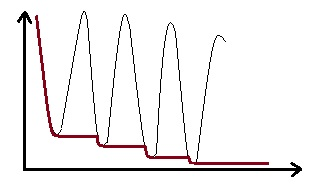
\includegraphics[width=0.5\textwidth]{Cri_graph1.jpg}
	\caption{lower bound}
	\label{fig:graph1}
	\end{figure}
	Now the other bound must be proved, so to reach the equality, but here there is a problem: $S_{N(t)}$ is not known, so it is difficult to demonstrate the inequality $t \geq S_{N(t)}$ since I cannot take the expectation. So we use a \textbf{trick}: we consider a new renewal process obtained by the previous one by truncation:
	\begin{equation}
	X_i^c =
	\begin{cases}
	X_i \qquad X_i \leq c\\
	c \qquad X_i >c
	\end{cases}
	\end{equation}

	What do we have for this truncated process?\\
	First of all we have the relations:
	\begin{equation}
	\begin{split}
	N^c(t) \geq N(t)\\
	M^c(t) \geq M(t)
	\end{split}
	\end{equation}
	because, since events are spaced by numbers that are no bigger, times are no smaller.\\

	So for the truncated process we have $t \geq S_{N^c(t) +1}$ (in the truncated process, the $X$ I'm adding cannot be bigger than $c$), and the next inequality also goes:
	\begin{equation}
	c+t \geq S_{N^c(t)+1}
	\end{equation}•
	If now I take this inequality expectation I obtain:
	\begin{equation}
	t+c \geq \mu^c(1+M^c(t))
	\end{equation}•
	and since $M^c(t) \geq M(t)$ from the previous inequality, I can say that:
	\begin{align}
	\begin{split}
	\mu^c(1+M^c(t)) \geq \mu^c(1+M(t))\\
	\frac{M(t)}{t} \leq \frac{1}{\mu^c} \frac{1}{t}(\frac{c}{\mu^c}-1) \qquad \forall c > 0 \quad (valid\quad for\quad any\quad truncation)
	\end{split}
	\end{align}

	NOTE: $c$ is an index, not an exponent.
	So now I take the limit:
	\beq
	\lim_{t \to \infty} sup \frac{M(t)}{t} \leq \frac{1}{\mu^c} \qquad \forall c > 0
	\eeq
	Since it is true $\forall c$ , it is true also for $c \to \infty$ (which means that truncation becomes less an less important until I don't truncate at all), so I obtain:
	\beq
	\lim_{t \to \infty} sup \frac{M(t)}{t} \leq \lim_{c \to \infty} \frac{1}{\mu^c}
	\eeq
	where $\mu^c = \int_0^c(1-F(x))\,dx$, so as $c \to \infty$ we see that $\mu^c \to \mu = \int_0^\infty(1-F(x))\,dx$. See figure\ref{fig:mu}
	\begin{figure}
	\centering
	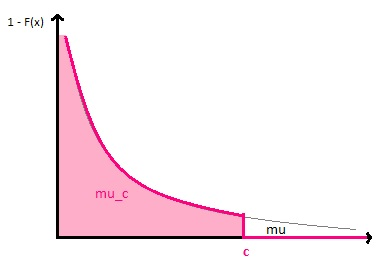
\includegraphics[width = 0.5\textwidth]{Cri_mu.jpg}
	\caption{This graph is the complementary distribution of $X^c$}
	\label{fig:mu}
	\end{figure}
	So at the end we conclude that
	\beq
	\lim_{t \to \infty} sup \frac{M(t)}{t} \leq \lim_{c \to \infty} \frac{1}{\mu^c} = \frac{1}{\mu}
	\eeq
	\\
	\textit{cvd}
	\subsection*{Observation}
	In the book, at the beginning, they assume that $E[X] < \infty$. Reasoning on it we can observe that:
	\begin{itemize}
	\item In the first part is not needed;
	\item In the second one, even though $\mu = 0$, I can make it finite by truncation;
	\end{itemize}
	\subsection{Two important results proofs}
	We now proceed with proving two important results:
	\begin{itemize}
	\item \textbf{1}: $E[S_{N(t)+1}] = (1+M(t))E[X]$;
	\item \textbf{2}: $E[S_{N(t)}] \ne M(t)E[X]$;
	\end{itemize}
	In the first case there is no case in which the equality is not true, so we can state that this equality is always true; in the second case there is a non-zero number of cases in which the equality is not true, and so it cannot taken as true in general.
	\subsubsection*{$1^{st}$ Statement}
	In this case represents a Poisson process: $S_{N(t)+1} = t + \gamma_t$ and $S_{N(t)} = t - \delta_t$;\\
	If i sit at time $t$, then $\gamma_t$ is the time until the next renewal, which means that the time until the next renewal occurs is $t + \gamma_t$, and so this is why $S_{N(t)}$ is the instant $t$ minus the time since the last renewal occurred $\delta_t$. And that's actually true for any renewal process.\\
	Moreover we know that both $\gamma$ and $\delta$ are exponentially distributed (because of Poisson process theory and the memoryless condition of the process): $\gamma_t$ is exponential with parameter $\lambda$, while $\delta_t$ is exponential with parameter $\lambda$ truncated at $t$.\\
	So we can find all the quantities involved:%min 25:00
	\beq
	E[S_{N(t)+1} = t + \frac{1}{\lambda}] \qquad E[S_{N(t)}] = t - \frac{1-e^{-\lambda t}}{\lambda}
	\eeq
	with $M(t) = \lambda t$ and $E[X] = \frac{1}{\lambda}$.\\
	Thanks to it we can see that the equality in true.
	\subsubsection*{$2^{nd}$ Statement}
	In this case we take:
	\beq
	X_i =
	\begin{cases}
	1 \qquad w.p. p\\
	a \geq 2 \qquad w.p. 1-p
	\end{cases}
	\eeq
	How many arrivals do we count?
	\beq
	N(t) =
	\begin{cases}
	1 \qquad w.p. p\\
	0 \qquad w.p. 1-p
	\end{cases}
	\eeq
	And how much time do we count?
	\beq
	S_{N(t)}=
	\begin{cases}
	1 \qquad w.p. p\\
	0 \qquad w.p. 1-p
	\end{cases}
	\eeq
	NOTE: Even though the value is the same, they do not represent the same thing.\\
	What about $S_{N(t)+1}$? $a>t$ so:
	\beq
	S_{N(t)+1} =
	\begin{cases}
	a \quad \text{w.p. $ (1-p)$}  \rightarrow \text{it means it the first renewal}\\
	2  \quad \text{w.p.  $p^2$}  \rightarrow \text{if the first  X is 1 and also the second}\\
	1+a \quad \text{w.p. $ p(1-p)$} \rightarrow \text{if the first X is 1 and the second is a}\\
	\end{cases}
	\eeq
	So:
	\beq
	\begin{split}
	E[S_{N(t)+1}] & = a(1-p)+2p^2+(1+a)p(1-p)\\
	                        & = p^2 + p + (1-p^2)a\\
	\end{split}
	\eeq
	\beq
	\begin{split}
	E[S_{N(t)}] & = p\cdot1 + 0\cdot(1-p)\\
		         & = p E[N(t)] = M(t)\\
		         & =  p\cdot1 + (1-p)\cdot0 = p
	\end{split}
	\eeq
	So I can try those equalities by multiplying
	\beq
	E[N(t)+1]E[X] = (1+p)(p+a(1-p)) = p^2+p+(1-p^2)a = E[S_{N(t)+1}]
	\eeq
	On the other hand:
	\beq
	E[N(t)]E[X] = p(p+(1-p)a) \ne p
	\eeq
	$\leftarrow$ {I can always find a value of $a$ that makes the equality not true}
	So the first equation was found to be true in both cases and it's contrary for the second.
	\subsection{Exercises}
	\subsubsection*{Ex 2.4}
	Each specific error is found on a specific case w.p. $\frac{1}{600}$ so the number of errors on given page is a binomial r.v. $(240,\frac{1}{600})$. At the same time, though, we know that when we have a Bin where $p$ is small and $M$ is big we can approximate it to a Poisson r.v. $\sim P(\frac{240}{600})$, where $\lambda = \frac{240}{600}  \simeq 0.4$.\\
	So I represent the book as:
	\begin{figure}[h]
	\centering
	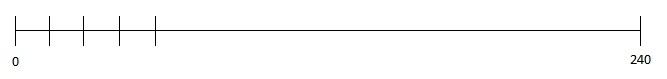
\includegraphics[width = 0.6\textwidth]{Cri_book.jpg}
	\label{fig:book}
	\end{figure}
	Easy to find the probability of what happens i different pages: each page is an independent interval, so:
	\beq
	P[\text{0 errors in 3 pages}\footnote{not necessarily consecutive}] = e^{-1.2}
	\eeq
	\subsubsection*{Ex 2.5}
	We have $N$ points equally distributed in a circle of radius $r$. The distribution of points in the circle of radius $1$ as $N \to \infty$ and $r \to \infty$ is:
	\beq
	\frac{N}{\pi r^2} < \lambda
	\eeq
	While the probability \textit{Prob[points inside r = 1]} is:
	\beq
	\frac{Small_{Area}}{Big_{Area}}
	\eeq
	This bring us to say that \textit{P[a given point is inside r $\leq$ 1] = } $\frac{Area(1)}{Area(r)} = \frac{1}{r^2}$.\\
	The number of points present in the smaller circle is a binary r.v. $\sim bin(N,\frac{1}{r^2})$, so its expected value is:
	\beq
	\text{E[number of points inside the smaller circle]} = \frac{N}{r^2} = \lambda\pi
	\eeq
	where $\lambda$ is the density of points and $\pi$ is the area of unitary circle.\\
	So we have two parameters, the product of which is still constant.
	\begin{align}
	\begin{split}
	N \to \infty \qquad r \to \infty\\
	\frac{N}{\pi r^2} = \lambda' \rightarrow P_{0i}(\lambda\pi)
	\end{split}
	\end{align}
	\subsubsection*{Ex 3.6}
	For $i = 1 \dots n$ I have an indep. PP $\rightarrow X_i(t)$ is an i.i.d. PP($\lambda$).\\
	The problem asks to find the first time such that there is at least one event  in every process, see figure\ref{fig:3.6}
	\begin{figure}[h]
	\centering
	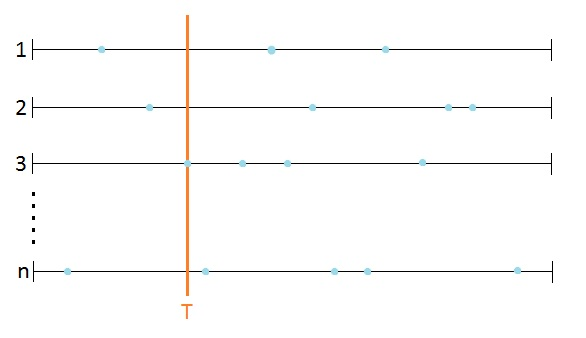
\includegraphics[width =0.6\textwidth]{Cri_Ex3_6.jpg}
	\label{3.6}
	\end{figure}
	Since the process is Poisson, we have that $P[T\leq t] = 1-P[0 events] = 1-e^{-\lambda t}$ for one process, while for $n$ processes we have $P[t \leq t] = (1-e^{}-\lambda t)^n$.\\
	We could actually see the problem from a different point of view: this view counts the events in the Poisson Poisson process and uses the independence to find the probability that none of them has seen $0$ events.\\
	So we can see how we can look at $T$: we get that $T$ is the time at which the last process has its first event and it will be the biggest value among the exponentials; the first event will occur, obviously, with exponential time, so using this reasoning we can express the r.v. $T$ as:
	\beq
	T = \max_{i = 1,2,\dots,n}{exp_i(\lambda)}
	\eeq
	So I can turn the point into a question: what is the distribution of the maximum among the i.i.d variables?
	\begin{align}
	\begin{split}
	P[max{X_1,X_2,\dots,X_n} \leq t] & = P[X_i \leq t, \quad i = 1,2, \dots, n]\footnote{since the X's are i.i.d.}\\
						  & = (P[X \leq t])^n = (1-e^{-\lambda t})^n
	\end{split}
	\end{align}
	In general this shows that if we take $F_{max}(t)$, then $F_{max}(t) = (F(t))^n$; on the other side:
	\begin{align}
	\begin{split}
	P[min{X_1,X_2,\dots,X_n} >t ] & = P[X_i > t \forall i = 1,2,\dots, n] \\
					        & = (P[X > t])^n
	\end{split}
	\end{align}
	So we found that $1-F_{min}(t) = (1-F(t))^n \rightarrow F_{min}(t) = 1- (1-F(t))^n$
	\subsubsection*{Problem 3.6}
	Service facility situation: service when $Q$ users arrived $\rightarrow$ a process that focuses on the $q^{th}$ arrival in sequence.\\
	$T = $ service time.
	\begin{figure}
	\centering
	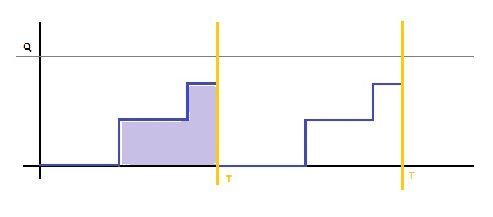
\includegraphics[width = 0.6\textwidth]{Cri_scale.jpg}
	\caption{Prob 3.6}
	\end{figure}
	We have to show that $E[\int_{0}^{T}N(t)dt] = \frac{q(Q-1)}{2\lambda}$; The first question is intuitive: we can see that if the time at which a user is served is the time at which the $q^{th}$ user arrives, then I have to wait for $q$ users to arrive to be served.\\
	I then have to take the expectation of the blue area, to do it I can use two different approaches: I can look how much time each user has to wait and then I sum all of then (and that corresponds to summing the horizontal slices of the area), or I can look at it vertically and see how much time there is one, two, three users waiting and then multiplying this amount of time by the number of users who are waiting during that time.\\
	So with the first approach:
	\begin{itemize}
	\item The first user will have to wait $\frac{1}{\lambda}(Q-1)$ inter-arrival times;
	\item The second user arrives after $2$ inter-arrival times and so he has to wait $\frac{1}{\lambda }(Q-2)$ inter-arrival times;
	\item After the second user more users will arrive until the $q^{th}$ user will arrive, and for it the waiting time will be $0$;
	\end{itemize}
	So the average sum of all the waiting time is the constant $1/\lambda$ times  the sum of the first $Q-1$ integers: $\frac{1}{\lambda}[(Q-1)+(Q-2)+\dots+1]$.\\
	With the second approach we see that:
	\begin{itemize}
	\item At the beginning no one is waiting in line;
	\item After the first arrival $1$ user is waiting;
	\item After the second arrival $2$ users are waiting;
	\item After the $(q)^{th}$ arrival, $Q-1$ users are waiting and so the structure is the same as previously.
	\end{itemize}
	\subsubsection*{Ex 4.1}
	Given $n$ arrivals, we take the quantity $E[w_1] = \int_{0}^{1}(1-t)^n dt = \frac{1}{n+1}$ where $w_1$ is the smallest among $n$ i.i.d. uniform r.v. between $0$ and $1$ and so the distribution is the distribution of the minimum of $n$ i.i.d. uniform r.v., and its complementary distribution is the $n^{th}$ power of the complementary distribution.\\
	\subsubsection*{Ex 4.3}
	Suppose we have $5$ arrivals, the cumulative time is the area in figure4, but we know that the arrival times are i.i.d. uniform so each user has to wait average waiting time is $0.5$ hours, so $0.5\times5 = 2.5$.\\
	\subsubsection*{Ex 4.5}
	Here assume we have $\alpha$  and the service time is an exponential r.v. $\sim exp(\alpha)$, and the probability $P[\text{at time 1 h the queue is empty}]$ is estimated considering each user arriving uniformly. So at the end the number of users is binomial and, conditioning on the uniform variable, we get:
	\begin{align}
	\begin{split}
	p = P & [\text{a uniformly arriving user has not left at time 1 h}] =\\
	& P[U_i + Y_i > 1] = \int_{0}^{1}e^{-\alpha(1-u)}du = \frac{1-e^{-\alpha}}{\alpha}
	\end{split}
	\end{align}
	So the probability becomes finding the probability that all users that had arrived here have left: it is the value $(1-P)^{n}$ with $n = $ \textit{number of users}:
	\begin{align}
	P&[\text{System empty at time 1|5 arrivals}] = (1-\frac{1-e^{-\alpha}}{\alpha})^5
	\end{align}
	\begin{figure}[h]
	\begin{minipage}[c]{0.5\textwidth}
	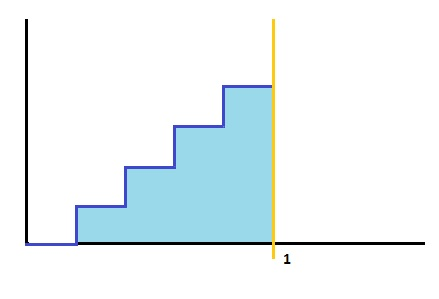
\includegraphics[width = 0.9\textwidth]{Cri_area.jpg}
	\caption{Ex 4.3}
	\end{minipage}
	\hspace{10mm}
	\label{fig:area}
	\begin{minipage}[c]{0.5\textwidth}
	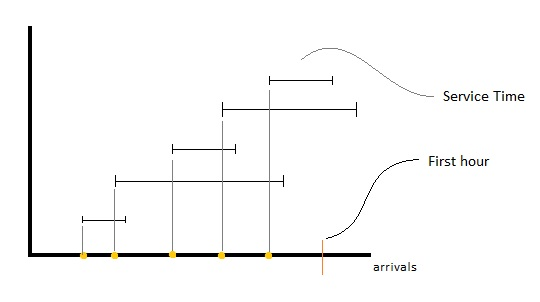
\includegraphics[width = 0.9\textwidth]{Cri_arrivals.jpg}
	\caption{Ex 4.5}
	\end{minipage}
	\end{figure}

\section{The key renewal theorem}
\begin{definition}
	(Point of increase) Given a distribution function F we call \textit{point of increase} every point $\alpha$ such that
	\begin{equation}
		F(\alpha+\epsilon)-F(\alpha-\epsilon)>0 \quad  \forall \quad
		\epsilon > 0
	\end{equation}
\end{definition}
\begin{definition}
	(Arithmetic function) We say that a distribution function F is \textit{arithmetic} if $\exists \lambda > 0$ such that F has points of increase exclusively among the points 0, $\pm \lambda$, $\pm 2\lambda$, \dots .

	We call \textit{SPAN} the largest $\lambda$ for which F is still arithmetic.
\end{definition}

The distribution function of a discrete random variable with possible values 0, 1, 2, \dots is an arithmetic function with SPAN=1.

\begin{definition}
	(Directly Riemann Integrable Function) Given a function g defined on [0, $\infty$) we define the following quantities for $\delta > 0$:
	\begin{align*}
		\underline \sigma (\delta) = \delta \cdot \sum_{n=1}^{\infty} min\{g(t):(n-1)\delta \leq t \leq n \delta \}
		\\
		\bar \sigma (\delta) = \delta \cdot \sum_{n=1}^{\infty}max\{g(t):(n-1)\delta \leq t \leq n \delta \}
	\end{align*}
	We say that g is directly Riemann integrable if both $\underline \sigma (\delta)$ and $\bar \sigma (\delta)$ converge absolutely $\forall \quad \delta > 0$ and if:
	\begin{equation}
		\underline \sigma (\delta) - \bar \sigma (\delta) \rightarrow 0 \quad \delta \rightarrow 0
		\end{equation}
\end{definition}

We note that every function for which $\int_{0}^{\infty} |g(t)| dt$ < $\infty$ (g is absolutely integrable) is directly Riemann integrable.

\begin{theorem}
	(Key Renewal Theorem) It is given a distribution function F of a positive random variable $a$ with mean $\mu$. We suppose that $a$ is directly Riemann integrable and that $A$ is the solution of the \textit{renewal equation}
	\begin{equation}
		A(t)=a(t)+\int_{0}^{t}A(t-x)dF(x)
	\end{equation}
	If F is not arithmetic, then
	\begin{equation*}
		\lim_{t \rightarrow \infty} A(t) =
		\begin{dcases}
			\frac{1}{\mu} \int_{0}^{\infty}a(x)dx \quad & if \quad \mu < \infty \\
			0 \quad & if \quad \mu = \infty
		\end{dcases}
	\end{equation*}
	If F is arithmetic with SPAN = $\lambda$ then, $\forall c > 0$
	\begin{equation*}
		\lim_{t \rightarrow \infty} A(c+n\cdot \lambda) =
		\begin{dcases}
			\frac{\lambda}{\mu} \sum_{n=0}^{\infty}a(c+n \cdot \lambda) \quad & if 	\quad \mu<\infty \\
			0 \quad & if \quad \mu = \infty
		\end{dcases}
	\end{equation*}
\label{KRT1}
\end{theorem}

The theorem \ref{KRT1} can be also expressed in the following form:

\begin{theorem}
	(Key renewal theorem) Is given a distribution function F of a positive random variable with mean $\mu$. We suppose $h>0$ and that $M(t)=\sum_{k=1}^\infty F_{k}(t)$ is the \textit{renewal function} associated with F.
	If F is not arithmetic then
	\begin{equation}
		\lim_{t \rightarrow \infty} [M(t+h)-M(t)]=\frac{h}{\mu}
	\end{equation}
	If F is arithmetic with SPAN = $\lambda$ then:
	\begin{equation}
		\lim_{t \rightarrow \infty} [M(t+h)-M(t)]=\frac{h}{\mu} \quad \forall h = n \cdot \lambda
	\end{equation}
	\label{KRT2}
\end{theorem}

We note that the \textit{elementary renewal theorem} $\lim_{t \to \infty} M(t) / t = 1 / \mu$ is a corollary of the \textit{key renewal theorem} \ref{KRT2}.

\subsection{Application of the key renewal theorem}

\paragraph{Limiting distribution of the excess life}

We say that $\gamma_{t}=S_{N(t)+1}-t$ is the excess life at time t and that $A_z=\prob[\gamma_t>z]$ for a fixed parameter $z>0$.

Conditioning on the first event, we obtain that
\begin{equation*}
	\prob[\gamma_t>z|X_1=x] = \begin{cases}
		1 \quad & if \quad x > t+z \\
		0 \quad & if \quad t+x \geq x > t \\
		A_z(t-x) \quad & if \quad t \geq x > 0
	\end{cases}
\end{equation*}

For the law of the total probability we have
\begin{align*}
	A_z(t) &= \int_{0}^{\infty} \prob[\gamma_t>z|X_1=x] dF(x) = \int_{0}^{t}A_z(t-x)dF(x)+\int_{t+z}^{\infty}dF(x)= \\
	&= \int_{0}^{t}A_z(t-x)dF(x)+ [1-F(t+z)]
\end{align*}

Now we apply the \textit{renewal equation} setting
\begin{equation} \begin{dcases}
	a(t) = 1 - F(t+z) \\
	A_z(t)=\int_{0}^{t} [1-F(t+z-x)] dM(x)+1-F(t+z)
\end{dcases} \end{equation}

\begin{align*}
	\int_{0}^{\infty} a(x) d(x) & = \int_{0}^{\infty}(1-F(x)) d(x) = \\
	& = \int_{z}^{\infty}(1-F(y))dy \leq \int_{0}^{\infty}(1-F(y))dy = \mu
\end{align*}

Supposing $\mu < \infty$, for the \textit{renewal theorem} we obtain that
\begin{equation}
	\lim_{t \rightarrow \infty} \prob[\gamma_t>z] = \lim_{t \rightarrow \infty} A_z(t) = \frac{1}{\mu} \cdot \int_z^{\infty}(1-F(x))dx \quad \forall z > 0
	\label{limitingdistribution}
\end{equation}

From \ref{limitingdistribution} we can determine the limiting distribution for the \textit{current life} $\delta_t$ and for the \textit{total life} $\beta_t$. First we note that
\begin{equation} \label{currtotallife}
	\{\gamma_t \geq x, \delta_t \geq y \}
	\Leftrightarrow
	\{\gamma_{t-y} \geq x+y \}
\end{equation}
From equation \ref{currtotallife} we have that
\begin{align*}
	\lim_{t \rightarrow \infty} \prob[\delta_t \geq y, \gamma_t \geq x] & = \lim_{t \rightarrow \infty} \prob[\gamma_{t-y} \geq x+y] \\ & = \frac{1}{\mu} \cdot \int_z^{\infty}(1-F(z))dz
\end{align*}
In particular we have that
\begin{align*}
	\lim_{t \rightarrow \infty} \prob[\delta_t \geq y] & = \lim_{t \rightarrow \infty} \prob[\delta_t \geq y, \gamma_{t} \geq 0] \\ & = \frac{1}{\mu} \int_z^{\infty}(1-F(z))dz
\end{align*}

So $\frac{1-F(z)}{\mu}$ is the probability density function of $\delta_t$. We are able to compute $\delta_t$ and $\gamma_t$ averages.
\begin{align*}
	\exp[\delta_t]=\exp[\gamma_t] & =\int_z^{\infty} \frac{z}{\mu} (1-F(z))dz \\ & = \frac{z^2}{2\mu} \left( 1-F(z) \right|_0^{\infty} + \int_0^{\infty}\frac{z^2}{2 \mu} f(z)dz= \frac{\exp[X^2]}{2 \exp[X]}
\end{align*}

Finally we conclude that
\begin{equation*}
	\begin{dcases}
		~ \exp[\delta_t] = \frac{\exp[X^2]}{2 \exp[X]} \\
		~ \exp[\gamma_t] = \frac{\exp[X^2]}{2 \exp[X]} \\
		~ \exp[\beta_t] = \frac{\exp[X^2]}{\exp[X]}
	\end{dcases}
\end{equation*}


\paragraph{Asymptotic expansion of the renewal function}
Given a distribution function $F$ of mean $\mu$ and variance $\sigma$ we want to find a more detailed description of the asymptotic behaviour of $M(t)$.

For $t \rightarrow \infty$ we have what follows
\begin{align*}
	M(t)-\frac{t}{\mu} & =\exp[N(t)+1]-\frac{t}{\mu}-1 \\
	& = \frac{1}{\mu} (\exp[S_{N(t)+1}]-t)-1 \\
	& = \frac{1}{\mu} \exp[\delta_t]-1 \\
	& = \frac{1}{\mu}\frac{\exp[X^2]}{2\mu}-1 \\
	& = \frac{\sigma^2+\mu^2}{2\mu^2}-1 \\
	& = \frac{\sigma^2-\mu^2}{2\mu^2}
\end{align*}

Then we finally prove that
\begin{equation}
	\lim_{t \rightarrow \infty} \left( M(t) - \frac{t}{\mu} \right) = \frac{\sigma^2-\mu^2}{2\mu^2}
\end{equation}

\subsection{Delayed renewal processes}
	We assume that $\{X_k\}$ are independent positive random variables but only $X_2,X_3,...$ are identically distribuited.
	In fact $X_1$ has a distribution function $G$ that differs from the distribution function $F$ of the other variables.

	We call such process \textit{delayed renewal process}. Given an ordinary renewal process we can obtain a \textit{delayed renewal process} if we fix the time origin $t=0$ a certain time after the start of the ordinary process.

	Let us put $S_0=0$ and $S_n=X_1+X_2+...+X_n$ and $N(t)$ equal to the number of renewal at time $t$. We must distinguish between the mean number of renewals in the delayed process $M_D(t)$ and the renewal function  $M(t)$ associated to $F$.

	\begin{align}
		& M_D(t) = \exp[N(t)]
		\\ & M(t) = \sum_{k=1}^{\infty}F_k(t)
	\end{align}
	Now we want to prove what follows:
	\begin{align*}
		& \lim_{t \to \infty }\frac{M_D(t)}{t}=\frac{1}{\mu}
		\\ & \lim_{t \to \infty }[M_D(t)-M_D(t-d)]=\frac{d}{\mu}
	\end{align*}

	We have already seen that for a recurrent irreducible aperiodic \gls{mc} the following statament is true.
	\begin{equation}
		\lim_{n \to \infty} P_{jj}^{(n)}=\pi_j=\frac{1}{m_j}=\frac{1}{\sum_{n=1}^{\infty}n \cdot f_{jj}^{(n)}}
	\end{equation}
	Given a recurrent state $j$ we call $N_j(t)$ the number of visits in $j$ by the time $t$. The following statament is always true for any initial state $Y_0$.

	\begin{equation}
		N_j(n)-N_j(n-1)=1 \quad \Leftrightarrow \quad Y_n=j
	\end{equation}

	If $Y_0$ is equal to j, then $N_j$ is a ordinary renewal process. We keep $Y_0=j$ and we obtain what follows.
	\begin{align*}
		& \exp[N_j(n)-N_j(n-1)|Y_0=j]=M(n)-M(n-1)=P_{jj}^{(n)}
		\\ & \Rightarrow \pi_j=\frac{1}{m_j}=\lim_{n \to \infty} P_{jj}^{n} = \lim_{n \to \infty} [M(n)-M(n-1)]=\frac{1}{\mu}
	\end{align*}

	So we have proved that
	\begin{equation}
		\lim_{n \to \infty} P_{jj}^{n}=\frac{1}{\mu}
	\end{equation}

	If $Y_0=i \neq j$, then $N_j(n)$ is a delayed renewal process. We keep $Y_0=i \neq j$ and we obtain what follows.
	\begin{align*}
		& \exp[N_j(n)-N_j(n-1)|Y_0=i \neq j]=M_D(n)-M_D(n-1)=P_{jj}^{(n)}
		\\ & \Rightarrow \frac{1}{\mu}=\lim_{n \to \infty} P_{jj}^{n} = \lim_{n \to \infty} [M_D(n)-M_D(n-1)]
	\end{align*}

	So we have proved that
	\begin{equation}
		\lim_{n \to \infty} [M_D(n)-M_D(n-1)]=\frac{1}{\mu} \Rightarrow \lim_{t \to \infty }\frac{M_D(t)}{t}=\frac{1}{\mu}
	\end{equation}

	Now we consider a periodic \gls{mc} with period $d$. We define $N_j$ as before. The following statament is always true for any initial state $Y_0$.
	\begin{equation}
		N_j(n \cdot d)-N_j((n-1)\cdot d)=1 \quad \Leftrightarrow \quad Y_{n \cdot d}=j
	\end{equation}

	For $Y_0=j$ we obtain what follows.
	\begin{align*}
		& \exp[N_j(n \cdot d)-N_j((n-1)\cdot d)|Y_0=j]=M(n \cdot d)-M((n-1)\cdot d)=P_{jj}^{(n \cdot d)}
		\\ & \Rightarrow d \cdot \pi_j=\frac{d}{m_j}=\lim_{n \to \infty} P_{jj}^{n \cdot d} = \lim_{n \to \infty} [ M(n \cdot d)- M( (n-1) \cdot d)]=\frac{d}{\mu}
	\end{align*}

	So we have proved that
	\begin{equation}
		\lim_{n \to \infty} P_{jj}^{n \cdot d}=\frac{d}{\mu}
	\end{equation}
	For $Y_0 \neq j$ we obtain what follows.
	\begin{align*}
		& \exp[N_j(n \cdot d)-N_j((n-1) \cdot d)|Y_0=i \neq j]=M_D(n \cdot d)-M_D((n-1) \cdot d)=P_{jj}^{(n \cdot d)}
		\\ & \Rightarrow \frac{d}{\mu}=\lim_{n \to \infty} P_{jj}^{n \cdot d} = \lim_{n \to \infty} [M_D(n \cdot d)-M_D((n-1) \cdot d)]
	\end{align*}
	So we have proved that
	\begin{equation}
		\lim_{n \to \infty} [M_D(n \cdot d)-M_D((n-1) \cdot d)]=\frac{d}{\mu} \Rightarrow \lim_{t \to \infty }[M_D(t)-M_D(t-d)]=\frac{d}{\mu}
	\end{equation}

\subsection{Cumulative and related renewal process}
	We associate to every random varriable $X_i$ a second random variable $Y_i$. So $Y_i$ and $X_i$ are dependent but the two couples $(X_i,Y_i)$ and $(X_j,Y_j)$ are still independent.

	We call $F$ the distribution function of $X_i$, $G$ the distribution function of $Y_i$, $\mu$ the mean of $X_i$ and $\nu$ the mean of $Y_i$.

	\paragraph{Queueing model}
	Suppose to have queueing system in which the arrivals follow a Poisson process. $X_i$ represents the the period between two consequent arrivals. $Y_i$ is a portion $X_i$ and represents the period in which the queieng system is busy. We call $p(t)$ the probability that $t$ falls into some portion $Y_i$. We suppose that the first interval has length $X_1=x$ and we obtain what follows.
	\begin{align*}
		p(t) & =\prob[t \in Y |X_1 = x]=\begin{dcases}
			\prob[Y_1>t|X_1=x] & \text{if} \quad x \geq t
			\\ p(t-x) & \text{if} \quad x<t
		\end{dcases}
		\\ & = \int_0^t p(t-x)dF(x)+\int_t^{\infty}\prob[Y_1>t|X_1=x]dF(x)
	\end{align*}
	Knowing that $\int_0^{t}\prob[Y_1>t|X_1=x]dF(x)=0$ we have that
	\begin{align*}
		p(t) & = \int_0^t p(t-x)dF(x)+\int_0^{\infty}\prob[Y_1>t|X_1=x]dF(x)
		\\ & = \prob[Y_1>t]+\int_0^t p(t-x)dF(x)
	\end{align*}

	We observe that $p(t)= \prob[Y_1>t]+\int_0^t p(t-x)dF(x)$ is a renewal equation. Let $\int_0^{\infty}\prob[Y_1>t]dt=\exp[Y_1]=\nu$, we can apply the renewal theorem
	\begin{align*}
		\lim_{t \to \infty} p(t) & = \frac{1}{\mu}\cdot\int_0^{\infty}p(t)dt = \frac{\nu}{\mu}= \frac{\exp[X]}{\exp[Y]}
	\end{align*}

\section{Renewal-Reward processes}
Consider a \textit{renewal process} $N(t)$ with interarrival time $X_n$ with distribution function $F$. We suppose that each time a renewal occurs we receive a \textit{reward}; we call $R_n$ the reward associated with the \emph{n}-th renewal event.

We suppose that each reward $R_n$ depends on the length of the interval $X_n$. In this scenario the pairs $(X_n, R_n)$ are independent and identically distribuited. We define the total number of reward $R(t)$ at time $t$ as follows.
\begin{equation}
	R(t)=\sum_{n=1}^{N(t)}R_n
\end{equation}
Now we adopt the following definitions.
\begin{align*}
	\exp[X] & =\exp[X_n]
	\\ \exp[R] & =\exp[R_n]
\end{align*}
\begin{theorem}[Th. 3.6 (Ross)]
  If $\exp[X]<\infty$ and $\exp[R]<\infty$ then with probability equal to 1 we have:
	\begin{equation}
		\lim_{t \to \infty}\frac{R(t)}{t}=\frac{\exp[R]}{\exp[X]}
		\label{rewardtheorem1}
	\end{equation}
	\begin{equation}
		\lim_{t \to \infty}\frac{\exp[R(t)]}{t}=\frac{\exp[R]}{\exp[X]}
		\label{rewardtheorem2}
	\end{equation}
\end{theorem}
\begin{proof} of equation \ref{rewardtheorem1}.
	\begin{align*}
		\frac{R(t)}{t}=\frac{\sum_{n=1}^{N(t)}R_n}{t}= \bigg( \frac{\sum_{n=1}^{N(t)}R_n}{N(t)}\bigg)\cdot\bigg(\frac{N(t)}{t}\bigg)
	\end{align*}
	By the strong law of large numbers we obtain that
	\begin{align*}
		\lim_{t \to \infty}\frac{\sum_{n=1}^{N(t)}R_n}{N(t)}=\exp[R]
	\end{align*}
	By the renewal theorem we obtain that
	\begin{align*}
		\lim_{t \to \infty} \frac{N(t)}{t}=\frac{1}{\exp[X]}
	\end{align*}
	Then \ref{rewardtheorem1} is proven.
\end{proof}
\begin{proof} of equation \ref{rewardtheorem2}.

	We see immediately that $N(t)+1$ is a stopping time both for $X_1,X_2,X_3,...$ and for $R_1,R_2,R_3,..$.
	\begin{align*}
		\sum_{n=1}^{N(t)}R_n \leq R(t) \leq \sum_{n=1}^{N(t)+1}R_n
	\end{align*}
	Then we have that
	\begin{align*}
		& \exp\bigg[\sum_{n=1}^{N(t)}R_n\bigg] \leq \exp[R(t)] \leq \exp\bigg[\sum_{n=1}^{N(t)+1}R_n\bigg]
		\\ & [M(t)+1] \, \exp[R]-\exp[R_{N(t)+1}] \leq \exp[R(t)] \leq [M(t)+1] \, \exp[R]
	\end{align*}
	Then, knowing that $\lim_{t \to \infty} \frac{[M(t)+1] \, \exp[R]}{t} = \frac {\exp[R]}{\exp[X]} $ we have that
	\begin{align*}
		\frac {\exp[R]}{\exp[X]} - \lim_{t \to \infty} \frac{\exp[R_{N(t)+1}]}{t} \leq \lim_{t \to \infty} \frac{\exp[R(t)]}{t} \leq \frac{\exp[R]}{\exp[X]}
	\end{align*}
	We put $A(t)=\exp[R_{N(t)+1}]$ and we have that
	\begin{align*}
		& \exp[R_{N(t)+1}|X_1=x]=
			\begin{cases}
				\exp[R_1|X_1=x] \quad & if \quad x>t
				\\ A(t-x) \quad & if \quad x \leq t
			\end{cases}
		\\ & \Rightarrow
		\\ & A(t)=\int_{0}^{t}A(t-x)dF(x)+\int_{t}^{+\infty}\exp[R_1|X_1=x]dF(x)
	\end{align*}
	We put $a(t)=\int_{t}^{+\infty}\exp[R_1|X_1=x]dF(x)$ and we have that
	\begin{align*}
		A(t)=\int_{0}^{t}a(t-x)dM(x)+a(t)=(M \ast a) (t)+a(t)
	\end{align*}
	Assuming that $R_n \geq 0$ we have that
	\begin{align*}
		& \lim_{t \to \infty}a(t) = \lim_{t \to \infty}\int_{t}^{+\infty}\exp[R_1|X_1=x]dF(x)=0
		\\ & a(0)=\int_{0}^{+\infty}\exp[R_1|X_1=x]dF(x)=\exp[R_1]<+\infty
	\end{align*}
	\begin{align*}
		|a(t)| & \leq \int_{t}^{+\infty}\exp[|R_1||X_1=x]dF(x)
		\\ & \leq \int_{0}^{+\infty}\exp[|R_1||X_1=x]dF(x) = \exp[|R_1|]=\exp[R_1]<+\infty
	\end{align*}
	So we have come to the following results:
	\begin{align*}
		1) \quad & \forall \epsilon>0 \quad \exists T>0:\quad |a(t)|<\epsilon \quad \forall t>T
		\\ 2) \quad & |a(t)| \leq \exp[|R_1|]<+\infty \quad \forall t
	\end{align*}
	Knowing that $A(t)=\int_{0}^{t}a(t-x)dM(x)+a(t)$ we have that
	\begin{align*}
		|A(t)| & = |\int_{0}^{t}a(t-x)dM(x)+a(t)| \leq \int_{0}^{t}|a(t-x)|dM(x)+|a(t)|
		\\ & \leq \int_{0}^{t-T}|a(t-x)|dM(x)+ \int_{t-T}^{t}|a(t-x)|dM(x) + a(t)
		\\ & \leq \int_{0}^{t-T}\epsilon dM(x)+ \int_{t-T}^{t}\exp[|R_1|] dM(x) + a(t)
	\end{align*}
	\begin{align*}
		\lim_{t \to \infty} \frac{A(t)}{t} \leq \lim_{t \to \infty} \epsilon \cdot \frac{M(t-T)}{t} + \lim_{t \to \infty} \exp[|R_1|]\cdot \frac{M(t)-M(t-T)}{t} + \lim_{t \to \infty} \frac{a(t)}{t}
	\end{align*}
	Knowing that $\lim_{t \to \infty} \epsilon \cdot \frac{M(t-T)}{t}=\frac{\epsilon}{\exp[X]}$, $\lim_{t \to \infty} \exp[|R_1|]\cdot \frac{M(t)-M(t-T)}{t}=0$ and $\lim_{t \to \infty} \frac{a(t)}{t}=0$ we have that
	\begin{align*}
		\lim_{t \to \infty} \frac{A(t)}{t} \leq \frac{\epsilon}{\exp[X]} \Rightarrow \lim_{t \to \infty} \frac{\exp[R_{N(t)+1}]}{t}=0 \Rightarrow \frac {\exp[R]}{\exp[X]} \leq \lim_{t \to \infty} \frac{\exp[R(t)]}{t} \leq \frac{\exp[R]}{\exp[X]}
	\end{align*}
	The we have that
	\begin{align*}
		\lim_{t \to \infty} \frac{\exp[R(t)]}{t} = \frac{\exp[R]}{\exp[X]}
	\end{align*}
	Then \ref{rewardtheorem2} is proven.
\end{proof}

Let us define the following quantities of interest.

\begin{equation*}
	\begin{dcases}
		r_{ij} & \text{reward of transition } i\rightarrow j \\
		R_{ij} = \exp[r_{ij}] & \text{mean reward of transition } i\rightarrow j\\
		R_i = \sum_k P_{ik} R_{ik} & \text{average reward of a visit to state } i\\
		\theta_{ij} =
			\begin{dcases}
				r_{ij} &\text{with probability } P_{ij}\\
				r_{ik}+\theta_{kj} &\text{with probability } P_{ik}, k\neq j
			\end{dcases}
			& \parbox[c]{.5\textwidth}{total reward going from $i$ to $j$ for the first time following any path} \\
			\begin{aligned}[b]
				\rho_{ij} &= \exp[\theta_{ij}] = \sum_{k=0}^{\infty}\exp[\theta_{ij}| X_1=k] P_{ik} =\\
				&= R_{ij}P_{ij} +\sum_{k \neq j} P_{ik} [R_{ik}+\rho_{kj}] \\
				&= R_i + \sum_{k \neq j}P_{ik}\rho_{kj}
			\end{aligned} & \parbox[b]{.5\textwidth}{average reward going from $i$ to $j$ for the first time following any path}
	\end{dcases}
\end{equation*}

We have that the average reward for transitions exiting each possible state $i$ is
\begin{equation*}
\sum_i \pi_i \rho_{ij} = \sum_i \pi_i R_i + \sum_i \sum_{k \neq j} \pi_i P_{ik} \rho_{kj} = \sum_j \pi_i R_i + \sum_{k \neq j}\rho_{kj}\sum_i\pi_i P_{ik}
\end{equation*}

For \emph{any} metric $r(\cdot)$ it holds that
\begin{equation}
\Rightarrow\sum_i \pi_i \rho_{ij} = \sum_j \pi_i R_i + \sum_{k \neq j}\pi_k\rho_{kj},\qquad \pi_j\rho_{jj} = \sum_i \pi_i R_i
\end{equation}

and if the metric is specifically \emph{time}
\begin{equation}
\pi_j \mu_{jj} = \sum_i \pi_i \mu_i
\end{equation}

Now, in system modeling one of the main task of performance evaluation is to find te average value of some reward over time, that is to evaluate $\lim_{t \to \infty}\frac{R(t)}{t}$. The following result holds:
\begin{equation}
\lim_{t \to \infty}\frac{R(t)}{t} = \frac{\exp[R]}{\exp[X]} = \frac{\rho_{jj}}{\mu_{jj}} = \frac{\sum_i \pi_i \frac{R_i}{\pi_j}}{\sum_i \pi_i \frac{\mu_i}{\pi_j}} = \frac{\sum_i \pi_i \sum_j P_{ik} R_{ik}}{\sum_i \pi_i \sum_k P_{ik}T_{ik}}
\end{equation}

This is a powerful way to evaluate systems performances, in order for this model to be applied two conditions need to be met:
\begin{enumerate}
	\item The system must be able to be modeled with a concept of \emph{state}\footnote{That's good for us, every protocol is essentially a state machine}
	\item The process must be Markovian or at least semi-Markovian
\end{enumerate}

\section{Regenerative Processes}

Consider a stochastic process $\{X(t), t \geq 0\}$ with state space $\{0, 1, 2, ... \}$ with the property that there exist time points at which the process (probabilistically) restarts itself.

That is, suppose that with probability 1, there exists a time $S_1$
such that the continuation of the process beyond $S_1$ is a probabilistic replica of the whole process starting at 0. Note that this property implies the existence of further times $S_2 , S_3 , \dots$ having the same property as $S_1$. Such a stochastic process is known as a \emph{regenerative process}.

From the above, it follows that $\{S_1 , S_2 , ...\}$ constitute the event times of a renewal process. We say that a cycle is completed every time a renewal occurs. Let $N(t) = \max\{n: S_n \leq t\}$ denote the number of cycles by time t.

\section{Semi-Markov Processes}
A semi-Markov process is one that changes states following a \gls{mc} but takes a random amount of time between changes.

More formally, consider a stochastic process with states $0, 1, ...  $, such that, whenever it enters state $i\geq 0$,
\begin{enumerate}
	\item The next state is $j$ with probability $P_{ij}$
	\item Given that the next state is $j$, the time the transition takes is random with distribution $F_{ij}$ and independent of past and future
\end{enumerate}
If we let $Z(t)$ denote the state at time $t$, then $\{Z(t), t\leq 0\}$ is called a \emph{semi-Markov
process}.
Thus a semi-Markov process does not possess the Markovian property that
the future is independent of the past, given the present state.

To predict the future not only would we want to know the present state, but also the length of time that has been spent in that state
\footnote{note that $Z(t) = \{\text{state of the process at time } t\}$ is a \gls{mc} only when the transition time is memoryless (for example exponential).}. Of course, at the moment of transition, all we would need to know is the new state (and nothing about the past).

Let $H_i(t)$ denote the \emph{distribution of time} that the semi-Markov process spends in state i before making a transition. For the law of total probability, we have that
\begin{equation}
	H_i(t) = \sum_j P_{ij} F_{ij}(t)
\end{equation}

and the average time between two consecutive transition in state $i$ is
\begin{equation}
	 \mu_i = \exp[H_i(t)] = \int_{0}^{+\infty}x \,dH_i(x)
\end{equation}

Let $T_{ii}$ denote the time between successive transitions into state $i$ and
\begin{equation}
\mu_{ii}=\exp [T_{ii}]
\end{equation}
With the theory of alternating renewal processes, it is a simple matter to derive an expression for the limiting probabilities of a semi-Markov process.

\begin{theorem}
	If the semi-Markov process is irreducible and if $T_{ii}$ has a non-lattice\footnote{previously defined as arithmetic} distribution with finite mean, then the limiting distribution

	$$P_j = \lim_{t \to \infty} \prob[Z(t)=j | Z(0)=k]$$

	exists and independent of the initial state. Furthermore,

	$$P_j = \frac{\exp[\mbox{time in state i in a cycle}]}{\exp[\mbox{duration of the cycle}]} = \frac{\mu_i}{\mu_{ii}}$$

\end{theorem}
Note that while $\mu_i$ is easy to compute, $\mu_{ii}$ is tipically much more difficult, since it requires the knowledge of the whole chain.

\section{Go Back N modeling}
%listen to the tape
From a modeling perspective, the packets subsequent to the bad packet are not relevant since we have to re transmit them either (See fig\ref{fig:gbns}). The transmitter will re transmit after two dashed packets so that two slots don't represent throughput since they are going to be rejected. To better understand, we number the packets and suppose to have a two-state Markov Channel:
\beq
\begin{cases}
0 \quad good\\
1 \quad bad
\end{cases}
\eeq
The channel matrix is:
\beq
C = \begin{bmatrix} p_{00} & p_{01}\\p_{10} & p_{11} \end{bmatrix}
\eeq
Every time the source try to retx, it does not do it right after the bad packet but only after a number of packets equivalent to the $R\pi(m)$. Doing so, this does not involve every single slot but some certain slots. The probability that, from the packet num $3$, the packet $4$ is good is a 1-step transmission probability; while the probability that the packet $3$ (coming after the packet $5$) is good is an m-step transmission probability. So we also write down the $m$ step matrix:
\beq
C^m =
\begin{bmatrix}
p_{00}(m) & p_{01}(m)\\
p_{10}(m) & p_{11}(m)
\end{bmatrix}\footnote{$p_{11}(m)$ is the probability of moving from a bad step to another bad step in $m$ moves}
\eeq
So we can model the protocol assuming error free feedback: (G = good, B = bad).
\begin{figure}
\centering
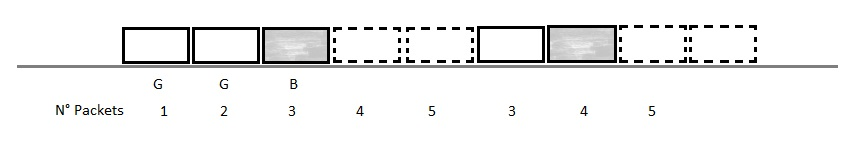
\includegraphics[width = .8\textwidth]{Cri_packets.jpg}
\caption{Go Back N scheme}
\label{fig:gbns}
\end{figure}
\begin{figure}
	\begin{center}
		\begin{tikzpicture}[->, >=stealth, auto, thin, node distance=3.5cm]
			\tikzstyle{every state}=[fill=white,draw=black,thin,text=black,scale=1]
			\node[state]		(G)											{$G$};
			\node[state]		(B)[right of=G]				{$B$};
			\path
			(G) 		edge[loop left]		 			node{$p_{00}$}				(G)
							edge[bend left]		 			node{$p_{01}$}		 		(B)
			(B)		edge[bend left]	node{$p_{01}(m)$}				(G)
							edge[loop right]					node{$p_{11}(m)$}	(B);

		\end{tikzpicture}
	\end{center}
	\caption{Graph model}
	\label{fig:GBN}
\end{figure}
In the model we can describe the behavior of the protocol like: \textit{If the slot is good, then go to the next one, otherwise skip $m-1$ slots and go to the $m^{th}$ one.}\\
With this reasoning it goes that the throughput is expressed as:
\beq
Throughput = \frac{\text{number of good slots}}{\text{total number of slots}}
\eeq
Every visit to state $G$ is $1$ success and every visit to state $B$ is a failure. The respective rewards are: $R_G = 1$ and $R_B = 0$; moreover we associate to $G$ and $B$ different time metrics: $T_{G} = 1$ and $T_{B} = m$, such that we obtain:
\beq
\lim_{t \to \infty}\frac{R(t)}{t} = \frac{\sum_i\pi_iR_i}{\sum_i\pi_iT_i}
\eeq
And the protocol chain is:
\beq
P =
\begin{bmatrix}
p_{00} & p_{01}\\
p_{10}(m) & p_{11}(m)
\end{bmatrix}
\eeq
To solve the limit we can find the $\pi$s like:
\begin{align}
\pi_{G} & = \frac{p_{10}(m)}{p_{10}(m)+p_{01}}\\
\pi_{B} & = \frac{p_{01}}{p_{10}(m)+p_{01}}
\end{align}
and insert them in the fraction, not considering the denominators, since they are the same for both the $\pi$s and so they would erase with each other.
\begin{align}
\begin{split}
\lim_{t \to \infty}\frac{R(t)}{t} & = \frac{\pi_GR_G+\pi_BR_B}{\pi_GT_G +\pi_BT_B}\\
& = \frac{p_{10}(m)\cdot1+p_{01}\cdot0}{p_{10}(m)\cdot1+p_{01}(m)}\\
& =\frac{p_{10}(m)}{p_{10}(m)+mp_{01}}
\end{split}
\end{align}
If we suppose an i.i.d. error we obtain:
\beq
\frac{1-\epsilon}{(1-\epsilon)+m\epsilon}
\eeq
Where $1-\epsilon$ is the \textit{P[having a good result | m previous results were bad]}, or better, \textit{P[having a good result]} since we hypothesized the independence of the errors.\\
Now let's try to answer another question: \textit{If we are in state G, how long does it take to us to come back?}\\
The answer is:
\beq
m_0 = p_{00}\cdot1+p_{01}[1+\frac{m}{p_{10}(m)}]
\label{Formula}
\eeq
Where $m_0$ is the average return time to $G$ and so the inverse of throughput; why? Because as in all semi-Markov processes, if we consider one state, visits to that one state are renewal instants. So the return time from $G$ to itself is a renewal interval and for this specific case, at every renewal cycle we have 1 success and the avg number of successes per unit time is the avg number of successes per cycle, $1$, divided by the average time per cycle. Moreover, once we have obtained the Markov structure we can identify the metrics we need to find.\\
Returning to the expression \ref{Formula}, for the part  inside the rectangular brackets, the expression means that we stay in $B$ for a geometric number of times, which is equal to the average inverse outgoing probability. What we obtain after some algebra\footnote{Fede e Davide this is for you $\heartsuit$} is:
\begin{align}
\begin{split}
m_0 & = 1+\frac{p_{01}\cdot m}{p_{10}(m)}\\
& = \frac{p_{10}(m)+mp_{01}}{p_{10}(m)}
\end{split}
\end{align}
\\
In the case the feedback has errors, we also need a M.C. for the acknowledgment and to combine it with the previous one, obtaining four states. But the only way to have successful transmission is that both the transmissions works fine:
\beq
C_f =
\begin{bmatrix}
p_{00} & p_{01}\\
p_{10} & p_{11}
\end{bmatrix}
\hspace{10mm}
C_b =
\begin{bmatrix}
q_{00} & q_{01}\\
q_{10} & q_{11}
\end{bmatrix}
\eeq
So the total transmission probability matrix is:
\beq
P =
\begin{bmatrix}
p_{00}q_{00} & p_{00}q_{01} & p_{01}q_{00} & p_{01}q_{01}\\
p_{00}(m)q_{10}(m) & p_{00}(m)q_{11}(m) & p_{01}(m)q_{10}(m) & p_{01}(m)q_{11}(m)\\
\text{$3^{rd}$ and} & \text{$4^{th}$ rows} & \text{can be} & \text{derived}\\
\text{in} & \text{a} & \text{similar} & \text{way}
\end{bmatrix}
\eeq
The state $00$ means $1$ success and $1$ slot, any other state is a failure: $0$ successes and $m$ slots. So I can rewrite the model, defining the vectors $R$ and $T$:
\beq
R =
\begin{bmatrix}
1\\
0\\
0\\
0
\end{bmatrix}
\hspace{20mm}
T =
\begin{bmatrix}
1\\
m\\
m\\
m
\end{bmatrix}
\eeq
and so obtaining the result:
\beq
\lim_{t \to \infty}\frac{R(t)}{t} = \frac{\bar{\pi}\bar{R}}{\bar{\pi}\bar{T}} = \frac{\pi_{00}\cdot 1}{\pi_{00}\cdot1+(1-\pi_{00})m}
\eeq
If now we suppose i.i.d. feedback errors w.p. $\delta$, we obtain the matrix
\beq
C_b =
\begin{bmatrix}
1-\delta & \delta\\
1-\delta & \delta
\end{bmatrix}
\eeq
Moreover, if the feedback channel is i.i.d., we have nothing to remember: regardless of whether the ack is good or bad, we do not care if the transmission was a failure $\rightarrow$ for this case we can use a simplified model with only $3$ states (figure\ref{fig:3states}), where the metrics are:
\beq
R =
\begin{bmatrix}
1\\
0\\
0
\end{bmatrix}
\hspace{5mm}
T =
\begin{bmatrix}
1\\
m\\
m
\end{bmatrix}
\eeq
\beq
p=
\begin{bmatrix}
(1-\delta)p_{00} & \delta p_{00} & p_{01}\\
(1-\delta)p{00}(m) & \delta p_{00}(m) & p_{01}(m)\\
(1-\delta)p_{10}(m) & \delta p_{10}(m) & p_{11}(m)
\end{bmatrix}
\eeq

\begin{figure}[h]
	\begin{center}
		\begin{tikzpicture}[->, >=stealth, auto, thin, node distance=4cm]
			\tikzstyle{every state}=[fill=white,draw=black,thin,text=black,scale=1]
			\node[state]		(G_0)											{$G_0$};
			\node[state]		(G_1)[below of=G]				{$G_1$};
			\node[state]		(B)[right of=G_1]		{$B$};
			\path
			(G_0) 	edge[loop left]	(G_0)
							edge[bend left=20]	(G_1)
							edge[bend left=20]	(B)
			(G_1)		edge[loop left]	(G_1)
							edge[bend left=20]	(G_0)
							edge[bend left=20]	(B)
			(B)			edge[loop right]	(B)
							edge[bend left=20]	(G_0)
							edge[bend left=20]	(G_1);
		\end{tikzpicture}
	\end{center}
	\caption{3-state model}
	\label{fig:3states}
\end{figure}
The throughput is:
\beq
\frac{\pi_{G_0}}{\pi_{G_0}+m(1-\pi_{G_0})}
\hspace{5mm}
\bar{\pi} = \bar{\pi}\cdot\bar{P}
\eeq
to obtain it we take:
\begin{align}
\pi_{G_0} & = (1-\delta)(\pi_{G_0}p_{00}+\pi_{G_1}p_{00}(m) +\pi_{B}p_{10}(m))\\
\pi_{G_1} & = \delta(\pi_{G_0}p_{00}+\pi_{G_1}p_{00}(m) +\pi_{B}p_{10}(m)) %Chiedere a Fede
\end{align}
where
\begin{itemize}
\item $(1-\delta)\pi_{G_1} = \delta\pi_{G_0}$
\item $(1-\delta)\pi_{B} = (1-\delta)-\pi_{G_0}$
\item $\pi_{B} = 1-\pi_{G_0}-\pi_{G_1} = 1-\pi_{G_0}-\frac{\delta}{1-\delta}\pi_{G_0} = 1- \frac{\pi_{G_0}}{1-\delta} = \frac{(1-\delta)-\pi_{G_0}}{1-\delta}$
\end{itemize}
and obtaining:
\begin{align}
\begin{split}
\pi_{G_0} & = (1-\delta)p_{00}\pi_{G_0} + \delta\pi_{G_0} p_{00}(m) (1-\delta-\pi_{G_0})p_{10}(m)\\
& = \frac{(1-\delta)p_{10}(m)}{1-(1-\delta)p_{00}-\delta p_{00}(m) +p_{10}(m)}
\end{split}
\end{align}
\beq
1-\pi_{G_0} = \frac{1-(1-\delta)p_{00} -\delta p_{00}(m) + \delta p_{10}(m)}{1-(1-\delta)p_{00}-\delta p_{00}(m) +p_{10}(m)}
\eeq
So the throughput is:
\beq
throughput = \frac{(1-\delta)p_{10}(m)}{(1-\delta)p_{10}(m) + m[1-(1-\delta)p_{00}-\delta p_{00}(m)+\delta p_{10}(m)]}
\eeq
\subsection{Graph reduction}
What if we rewrite the scheme, such that we can reduce it like in figure\ref{fig:GBN}?\\
From a memory point of view it is ok because we do not need to keep memory of the acknowledgments since they are i.i.d; but let's try to understand what happens in terms of success or failure of the acknowledgments:
\\
If we enter state $G$ (we tx a packet and it is succesful)we have:
\begin{itemize}
\item The ack is correct and we found $1$ success in $1$ slot w.p. $1-\delta$;
\item W.p. $\delta$ instead, we count $0$ successes in $m$ slots;
\end{itemize}
This brings us to conclude that in state $G$ we have:
\begin{itemize}
\item $1$ reward w.p. $1-\delta$, $0$ otherwise;
\item $1$ slot w.p. $1-\delta$, $m$ otherwise;
\end{itemize}
About transition probabilities:
\begin{itemize}
\item going to $G$ w.p. $(1-\delta)p_{00}+\delta p_{00}(m)$;
\item going to $B$ w.p. $(1-\delta)p_{01}+\delta p_{01}(m)$;
\end{itemize}
In state $B$ we have:
\begin{itemize}
\item No reward w.p. $1$ and $m$ slots always;
\item We go from there to $G$ w.p. $p_{10}(m)$;
\item And to $B$ w.p. $p_{11}(m)$;
\end{itemize}
So now we have a simplified Markov model where we combine into a single state everything that before was separate. What we obtain is:
\beq
\pi_{G} = \frac{p_{10}(m)}{(\dots)}
\hspace{20mm}
\pi_{B} = \frac{(1-\delta)p_{01}+\delta p_{01}(m)}{(\dots)}
\eeq
Reward and time:
\beq
R =
\begin{bmatrix}
1-\delta\\
0
\end{bmatrix}
\hspace{20mm}
T =
\begin{bmatrix}
1-\delta+\delta \cdot m\\
m
\end{bmatrix}
\eeq
And finally we can estimate the throughput for the system in figure\ref{fig:2states}:
\beq
\lim_{t \to \infty} \frac{R(t)}{t} = \frac{\bar{\pi}\bar{R}}{\bar{\pi}\bar{T}} = \frac{(1-\delta)p_{10}(m)}{(1-\delta+\delta \cdot m)p_{10}(m)+m[(1-\delta)p_{01}+\delta p_{01}(m)]}
\eeq
We just note that the denominator of this expression is equal to the one in the previous throughput expression: to prove it it is necessary to impose:
\begin{itemize}
\item $p_{00} = 1-p_{01}$;
\item $p_{00}(m) = 1-p_{01}(m)$
\end{itemize}
So $1-(1-\delta)p_{00}-\delta p_{00}(m) = (1-\delta)p_{01} + \delta p_{01}(m)$.\\
This result stands out from the fact that the two throughputs are the same quantity but computed by two different models; so we did not reduced the complexity, we just redistributed the quantities.

\begin{figure}[h]
	\begin{center}
		\begin{tikzpicture}[->, >=stealth, auto, thin, node distance=3.5cm]
			\tikzstyle{every state}=[fill=white,draw=black,thin,text=black,scale=1]
			\node[state]		(G)											{$G$};
			\node[state]		(B)[right of=G]				{$B$};
			\path
			(G) 		edge[loop left]		 			node{$(1-\delta)p_{00}+\delta p_{00}(m)$}				(G)
							edge[bend left=20]		 			node{$(1-\delta)p_{01} + \delta p_{01}(m)$}		 		(B)
			(B)		edge[bend left=20]	node{$p_{10}(m)$}				(G)
							edge[loop right]					node{$p_{11}(m)$}	(B);

		\end{tikzpicture}
	\end{center}
	\caption{2-state simplified model}
	\label{fig:2states}
\end{figure}

\chapter{Markov Error Process}
Two state Markov process $X_n$: 0 = correct transmission, 1 = erroneous transmission. Statistic of successful slots up to time n:
\begin{equation}
	\begin{split}
			\Phi_{ij}(k,n) = & \prob[\textrm{k good slots in 0,1,$\dots$,n-1 and j at n | i at 0}] \\
										 = & \prob\left[\sum\limits_{m=0}^{n-1} \mathds{1}\{X_m = 0\} = k, X_n = j | X_0 = i\right]
	\end{split}
\end{equation}
\paragraph{Conditioning on last transition}
If the last state is successfull, we require $k-1$ successes in the previous $n-1$ transitions, else we require $k$ successes in the previous $n-1$ successes:
$$\Phi_{ij}(k,n) = \Phi_{i0}(k-1,n-1)P_{0j} + \Phi_{i1}(k,n-1)P_{1j} \textrm{ with } n>0 \textrm{ and } 0<k\leq n$$
Initial condition:
\begin{equation}
 \begin{split}
	 &\Phi_{ij}(k,0)=
	 \begin{cases}
		 1 &  \text{if } i = j \text{and } k = 0 \\
		 0 &  \text{otherwise}
	 \end{cases}
 \end{split}
\end{equation}
Using the $\delta$ functions:
\begin{equation*}
 \begin{split}
	 &\delta_{ij}=
	 \begin{cases}
		 1 &  \text{if } i = j \\
		 0 &  \text{otherwise}
	 \end{cases}
 \end{split}
\end{equation*}
and
\begin{equation*}
 \begin{split}
	 &\delta(k)=
	 \begin{cases}
		 1 &  \text{if } k = 0 \\
		 0 &  \text{otherwise}
	 \end{cases}
 \end{split}
\end{equation*}
The initial condition can be rewritten as: $\Phi_{ij}(k,0)=\delta_{ij}\delta(k)\delta(n)$.\\
Therefore $\Phi_{ij}(k,n) = 0$ if $k<0$ or $k>n$ or $n<0$.\\
Finally:
$$\Phi_{ij}(k,n) =  \Phi_{i0}(k-1,n-1)P_{0j} + \Phi_{i1}(k,n-1)P_{1j} + \delta_{ij}\delta(n)\delta(k)$$
In matrix form: $\Phi(k,n) = \begin{pmatrix} \Phi_{00}(k,n)&\Phi_{01}(k,n)\\ \Phi_{10}(k,n)&\Phi_{11}(k,n)\end{pmatrix}$
\begin{equation}
	\begin{split}
			\Phi(k,n) =	 & \Phi(k-1,n-1)\underbrace{\begin{pmatrix} P_{00}&P_{01}\\0&0 \end{pmatrix}}_{\mathclap{= P(1)\text{ (``good transitions'')}}} + \Phi(k,n-1)\underbrace{\begin{pmatrix} 0&0\\ P_{10}&P_{11}\end{pmatrix}}_{\mathclap{=P(0)\text{ (``bad transitions'')}}} + I\delta(n)\delta(k)\\
								= & \Phi(k-1,n-1)P(1) + \Phi(k,n-1)P(0) + I\delta(n)\delta(k)
	\end{split}
\end{equation}
If, instead, we condition on the first transition:
\begin{align*}
\Phi_{0j}(k,n) =& P_{00}\Phi_{0j}(k-1, n-1) + P_{01}\Phi{1j}(k-1,n-1) + \delta_{0j}\delta(n)\delta(k)  \\
\Phi_{1j}(k,n) =& P_{10}\Phi_{0j}(k, n-1) + P_{11}\Phi{1j}(k,n-1) + \delta_{1j}\delta(n)\delta(k)
\end{align*}
In matrix form: $\Phi(k,n) = P(1)\Phi(k-1,n-1) + P(0)\Phi_{i1}(k,n-1) + I\delta(n)\delta(k)$.\\
To solve these equations:
\begin{itemize}
	\item compute recursively (brute force)
	\item use transforms
\end{itemize}
2D transform of $\Phi(k,n)$: $\varphi(s,z) = \sum\limits_{k=0}^{+\infty}s^k\sum\limits_{n=0}^{+\infty}z^n\Phi(k,n)$ \\
Using transforms properties: $\varphi(s,z) = \varphi(s,z)P(1)sz + \varphi(s,z)P(0)z + I $ \\
Therefore:
\begin{equation}
\begin{split}
	\varphi(s,z) = & [I - P(1)sz -P(0)z ]^{-1} \\
							 = & [I - z(P(1)s + P(0))]^{-1} \\
							 = & \sum\limits_{n=0}^{+\infty}[P(1)s + P(0)]^n z^n
\end{split}
\end{equation}
$$\rightarrow \varphi(s,n)= \underbrace{\sum\limits_{k=0}^{+\infty} s^k \Phi(k,n)}_{\mathclap{\text{transform over k for a given n}}}=(P(1)s+P(0))^n$$
Now suppose we associate an integer metric to each transition. Let $P(l)$ be the matrix that contains all elements of P that correspond to a ``reward'' of l. We have:
$$\Phi(k,n) = \sum\limits_{l=0}^{+\infty} \Phi(k-l,n-1)P(l) + I\delta(n)\delta(k)$$
With transform: $\varphi(s,z) = \varphi(s,z)\psi(s)z + I$.\\
Where
\begin{equation}
\begin{split}
		\psi(s) =& \sum\limits_{l=0}^{+\infty} P(l)s^l \\
						=& P(1)s + P(0) \text{  (in the previous case)}
\end{split}
\end{equation}
As before: $\varphi(s) = [I - z\psi(s)]^{-1} \rightarrow \varphi(s,n)=[\psi(s)]^n$ for a given n.\\
\textbf{Notes:}
\begin{enumerate}
	\item We can find average number of rewards in 0,1,...,n-1 as before
	\item In $\varphi(s,z)$, s labels successes and z labels the number of transitions
	\item Each transition has a ``label'' $\psi_{ij}(s)$
	\item The label $\psi_{ij}(s)$ does not need to be a single term, but in general can be polynomial: $$\psi_{ij}(s) = \sum\limits_{l=0}^{+\infty} P_{ij}(l)s^l$$
				Where $P_{ij} = \prob[X_{n+1}=j\text{ and l is earned}| X_n = i]$.\\
				Properties of $\psi_{ij}(s)$:
				\begin{itemize}
					\item[a)] $\psi_{ij}(1)=P_{ij} \rightarrow \text{in matrix form: } \psi(1) = P$
					\item[b)] $\frac{\psi_{ij}(s)}{P_{ij}}=\text{generating function of the distribution of the metric given the transition}$
					\item[c)] $\psi_{ij}^{'}(1)=P_{ij}\E[\text{reward earned in the transition from i to j}] $
					\item[d)] If the metric is the reward:
								\begin{equation}
									\begin{split}
										R_i =& \sum_j P_{ij}R_{ij} \\
										    =& \sum_j \psi_{ij}^{'}(1)
									\end{split}
								\end{equation}
				\end{itemize}
	\item We can define multiple metrics, i.e., $\textbf{s} = (s_1,...)$. In this case,
				$$P_{ij}\E[\text{k-th metric on transition } i \rightarrow j] = \frac{\partial \psi_{ij}(s_1,...)}{\partial s_k}\bigg|_{\textbf{s}=\textbf{1}} $$
				$$R_{ij}^{(k)}P_{ij}=  \frac{\partial \psi_{ij}(s)}{\partial s_k}\bigg|_{\textbf{s}=\textbf{1}}$$
				$$R_i^{(k)} = \sum_j P_{ij}R_{ij}^{(k)} = \sum_j \frac{\partial \psi_{ij}(s)}{\partial s_k}\bigg|_{\textbf{s}=\textbf{1}}$$
				$$ \lim_{t \to \infty}\frac{R^{(1)}(t)}{R^{(2)}(t)}=\frac{\sum_i \pi_i R_i^{(1)}}{\sum_i \pi_i R_i^{(2)}}= \frac{\mathbf{\pi} \frac{\partial \psi(\mathbf{s})}{\partial s_1}\bigg|_{\textbf{s}=\textbf{1}}\textbf{1}}{\mathbf{\pi}\frac{\partial \psi(\mathbf{s})}{\partial s_2}\bigg|_{\textbf{s}=\textbf{1}}\textbf{1}}$$
	\item To compute $\psi_{ij}(s)$:
		\begin{itemize}
			\item[a)] Let $\epsilon(i,j)$ be the set of all events that lead from state i to state j
			\item[b)] Let $\prob[A]$ be the probability of each event A
			\item[c)] Let $\textbf{s}(A) = s_1^{l_1(a)}s_2^{l_2(A)}...$ where $l_k(A)$ is the value of the k-th metric that corresponds to the event A
			\item[d)] We have: $$\psi_{i,j}(\textbf{s}) = \sum_{A \in \epsilon(i,j)} \prob[A]\textbf{s}(A)$$
			$$\psi_{i,j}(\mathbf{1}) =\sum_{A \in \epsilon(i,j)} \prob[A] = P_{ij}$$
		\end{itemize}
\end{enumerate}


\chapter{Go Back N protocol with limited retransmissions}
Suppose a system governed by the Go Back N protocol.
In this system the \gls{rtt} take m slot and when a received packet is wrong, it's retransmitted, until the $N^{th}$ failure, after which the packet is discarded.

$x(t)$ is the random variable indicating the state of the system. The possible values of $x(t)$ can be:

$$ x(t) = G \text{ \qquad if success at t} $$
$$ x(t) = B_j \text{ \qquad if $j_{th}$ failure at t} $$

Where we count a success whenether we enter in state $G$.
In the following system, we define 2 metrics:

$$s_1 = \text{number of success per transition}$$
$$s_2 = \text{time per transition}$$

\begin{figure}[h]
	\begin{center}
		\begin{tikzpicture}[->, >=stealth, auto, thin, node distance=3.5cm]
			\tikzstyle{every state}=[fill=white,draw=black,thin,text=black,scale=1]
			\node[state]		(G)											{$G$};
			\node[state]		(B_1)[right of=G]				{$B_1$};
			\node[state]		(B_2)[right of=B_1]			{$B_2$};
			\node[state]		(dots)[right of=B_2]		{...};
			\node[state]		(B_N)[right of=dots]		{$B_N$};
			\path
			(G) 		edge[loop left]		 			node{$P_{00}s_1s_2$}			(G)
							edge[bend left]		 			node{$P_{01}s_2$}		 			(B_1)
			(B_1)		edge[bend left]					node{$P_{10}(m)s_1s_2^m$}	(G)
							edge[bend left, below]	node{$P_{11}(m)s_2^m$}		(B_2)
			(B_2)		edge[bend left]																		(G)
							edge[bend left, below]	node{$P_{11}(m)s_2^m$} 		(dots)
			(dots)	edge[bend left, below]	node{$P_{11}(m)s_2^m$} 		(B_N)
							edge[bend left]																		(G)
			(B_N)		edge[bend left]																		(G)
			(B_N)		edge[bend right, above]	node{$P_{11}(m)s_2^m$}		(B_1);
		\end{tikzpicture}
	\end{center}
	\caption{Markov Chain of the Go Back N protocol with limited retransmission}
	\label{fig:gbn_mc_complete}
\end{figure}

We spend 1 slot in $G$ and m slots in $B_j$ since we need an \gls{rtt} to recognize an error.

For the sake of simplicity we rename the transition probability in a simpler way:
$$ \beta_{00} = P_{00}s_1s_2 \qquad \beta_{01} = P_{01}s_2$$
$$ \beta_{10} = P_{10}(m)s_1s_2^m \qquad \beta_{11} = P_{11}(m)s_2^m$$

All these $\beta s$ seems similar, we can simplify a bit the system assuming the following statement:

\begin{enumerate}
	\item metrics on different transitions are independent;
	\item metrics are additive;
	\item the transform of the distribution of sum is the product of the transforms.
\end{enumerate}

In the following part there are some example to show how the semplification work.

Given a three-state system $x(t) = i,j,k$, we want to reduce it to a two-state system.

\begin{center}
	\begin{tikzpicture}[->, >=stealth, auto, thin, node distance=3.5cm]
		\tikzstyle{every state}=[fill=white,draw=black,thin,text=black,scale=1]
		\node[state]		(i)								{$i$};
		\node[state]		(j)[right of=i]		{$j$};
		\node[state]		(k)[right of=j]		{$k$};
		\path
		(i) 		edge[bend left]		node{$P_{ij}\frac{\Psi_{ij}(s)}{P_{ij}}$}			(j)
		(j) 		edge[bend left]		node{$P_{jk}\frac{\Psi_{jk}(s)}{P_{jk}}$}			(k);

	\end{tikzpicture}
\end{center}

$$ \Psi_{ij}(s) = \sum_{A \in \epsilon(i,j)} P[A] \cdot \mathbf{S}[A] \qquad \Psi_{jk}(s) = \sum_{B \in \epsilon(j,k)} P[B] \cdot \mathbf{S}[B]$$

Using the assumption made before, we can reduce the above system to a two-state system with the product of the transition probabilities $\Psi_{ij}(s)$ and $\Psi_{jk}(s)$ as transition probability.

\begin{center}
	\begin{tikzpicture}[->, >=stealth, auto, thin, node distance=3.5cm]
		\tikzstyle{every state}=[fill=white,draw=black,thin,text=black,scale=1]
		\node[state]		(i)								{$i$};
		\node[state]		(k)[right of=i]		{$k$};
		\path
		(i) 		edge[bend left]		node{$\Psi_{ik}(s)$}			(k);

	\end{tikzpicture}
\end{center}

$$ \Psi_{ik}(s) = \Psi_{ij}(s) \cdot \Psi_{jk}(s) = \sum_{A \in \epsilon(i,j), B \in \epsilon(j.k)} P[A] \cdot P[B] \cdot \mathbf{S}[A] \cdot \underline{S}[A]$$

What if we are in the following situation?

\begin{center}
	\begin{tikzpicture}[->, >=stealth, auto, thin, node distance=3cm]
		\tikzstyle{every state}=[fill=white,draw=black,thin,text=black,scale=1]
		\node[state]		(i)								{$i$};
		\node[state]		(j)[right of=i]		{$j$};
		\node[state]		(k)[above right of=j]		{$k$};
		\node[state]		(l)[below right of=j]		{$l$};
		\path
		(i) 		edge		node{$\Psi_{ij}$}			(j)
		(j) 		edge[left]		node{$\Psi_{jk}$}			(k)
						edge[left]		node{$\Psi_{jl}$}			(l);

	\end{tikzpicture}
\end{center}

In this case we can substitute state $j$ with 2 different paths starting from $i$ and ending in $k$ and $l$, considering as transition probability the product of the initial transition probabilities, as is shown in the following figure.

\begin{center}
	\begin{tikzpicture}[->, >=stealth, auto, thin, node distance=3cm]
		\tikzstyle{every state}=[fill=white,draw=black,thin,text=black,scale=1]
		\node[state]		(i)								{$i$};
		\node[state]		(k)[above right of=i]		{$k$};
		\node[state]		(l)[below right of=i]		{$l$};
		\path
		(i) 		edge[left]		node{$\Psi_{ij}\Psi_{jk}$}			(k)
						edge[left]		node{$\Psi_{ij}\Psi_{jl}$}			(l);

	\end{tikzpicture}
\end{center}

With this rule we can remove states $B_2, B_3, \cdots, B_{N-1}$ from the system represented in \autoref{fig:gbn_mc_complete}, and reduce it to the system represented in \autoref{fig:gbn_mc_3state}.

\begin{figure}[h]
	\begin{center}
		\begin{tikzpicture}[->, >=stealth, auto, thin, node distance=3.5cm]
			\tikzstyle{every state}=[fill=white,draw=black,thin,text=black,scale=1]
			\node[state]		(G)											{$G$};
			\node[state]		(B_1)[right of=G]				{$B_1$};
			\node[state]		(B_N)[right of=B_1]		{$B_N$};
			\path
			(G) 		edge[loop left]		 			node{$\beta_{00}$}				(G)
							edge[bend left]		 			node{$\beta_{01}$}		 		(B_1)
			(B_1)		edge[bend left, above]	node{$\beta_{BG}$}				(G)
							edge[bend left]					node{$\beta_{11}^{N-1}$}	(B_N)
			(B_N)		edge[bend left]					node{$\beta_{10}$}				(G)
							edge[bend left, above]	node{$\beta_{11}$}				(B_1);

		\end{tikzpicture}
	\end{center}
	\caption{\autoref{fig:gbn_mc_complete} reduced to 3-state system}
	\label{fig:gbn_mc_3state}
\end{figure}

Where $\beta_{BG}$ takes in account all the possible paths from $B_1$ to $G$ and is define as:

\begin{equation}
	\beta_{BG} = \beta_{10} + \beta_{11}\beta_{10} + \beta_{11}^2\beta_{10} + \cdots + \beta_{11}^{N-2}\beta_{10} = \beta_{10}\sum_{k=0}^{N-2} \beta_{11}^K = \beta_{10}\frac{1-\beta_{11}^{N-1}}{1-\beta_{11}}
\end{equation}

What about removing $B_N$?
To reduce \autoref{fig:gbn_mc_3state} to a 2-state system we need one more property.

In the case that we have 2 transitions towards the same state, we can sum the transition probabilities as in the following example.

\begin{center}
	\begin{tikzpicture}[->, >=stealth, auto, thin, node distance=3cm]
		\tikzstyle{every state}=[fill=white,draw=black,thin,text=black,scale=1]
		\node[state]		(i)								{$i$};
		\node[state]		(j)[right of=i]		{$j$};
		\node		(ar)[right of=j]		{$\Rightarrow$};
		\node[state]		(i1)[right of=ar]		{$i$};
		\node[state]		(j1)[right of=i1]		{$j$};
		\path
		(i) 		edge[bend left]		node{$\Psi_{ij}^{(1)}$}			(j)
						edge[bend right, below]		node{$\Psi_{ij}^{(2)}$}			(j)
		(i1)		edge							node{$\Psi_{ij}^{(1)} + \Psi_{ij}^{(2)}$} (j1);

	\end{tikzpicture}
\end{center}

Knowing the previous property, we can remove $B_N$ from \autoref{fig:gbn_mc_3state}.

\begin{figure}[h]
	\begin{center}
		\begin{tikzpicture}[->, >=stealth, auto, thin, node distance=3.5cm]
			\tikzstyle{every state}=[fill=white,draw=black,thin,text=black,scale=1]
			\node[state]		(G)											{$G$};
			\node[state]		(B_1)[right of=G]				{$B_1$};
			\path
			(G) 		edge[loop left]		 			node{$\beta_{00}$}				(G)
							edge[bend left]		 			node{$\beta_{01}$}		 		(B_1)
			(B_1)		edge[bend left]	node{$\beta_{BG} + \beta_{10}\beta_{11}^{N-1}$}				(G)
							edge[loop right]					node{$\beta_{11}^{N}$}	(B_1);

		\end{tikzpicture}
	\end{center}
	\caption{\autoref{fig:gbn_mc_complete} reduced to 2-state system removing the state $B_N$.}
	\label{fig:gbn_mc_2state}
\end{figure}

In \autoref{fig:gbn_mc_2state} we can rearrange the probability of going from $B_1$ to $G$ in the following way:

\begin{equation}
	\beta_{BG} + \beta_{10}\beta_{11}^{N-1} = \beta_{10}\sum_{K=0}^{N-1} \beta_{11}^K = \beta_{10}\frac{1-\beta_{11}^N}{1-\beta_{11}}
\end{equation}

At the end of this process we want to reduce \autoref{fig:gbn_mc_complete} to a one-state system.
In the previous steps we have reduced \autoref{fig:gbn_mc_complete} to a two-state system, we still have to remove $B_1$ from \autoref{fig:gbn_mc_2state}.

To perform this, we have to make a further example.

Suppose you have three states in the following configuration:

\begin{center}
	\begin{tikzpicture}[->, >=stealth, auto, thin, node distance=3cm]
		\tikzstyle{every state}=[fill=white,draw=black,thin,text=black,scale=1]
		\node[state]		(x)								{$x$};
		\node[state]		(z)[right of=x]		{$z$};
		\node[state]		(y)[right of=z]		{$y$};
		\path
		(x)		edge		node{$a$}			(z)
		(z)		edge[loop, above]	node{$b$} (z)
					edge		node{$c$} (y);

	\end{tikzpicture}
\end{center}

In this case, the probability to found the system in state $z$ (i.e. $p(z)$) will be

\begin{equation}
	p(z) = ap(x)+bp(z)
\end{equation}

And so, rearranging this formula, we obtain

\begin{equation}
	p(z) = \frac{ap(x)}{1-b} \qquad and \qquad p(y) = cp(z) = \frac{acp(x)}{1-b}
\end{equation}

With this method we have remove state $z$, remaining with only one transition from $x$ to $y$:

\begin{center}
	\begin{tikzpicture}[->, >=stealth, auto, thin, node distance=3cm]
		\tikzstyle{every state}=[fill=white,draw=black,thin,text=black,scale=1]
		\node[state]		(x)								{$x$};
		\node[state]		(y)[right of=x]		{$y$};
		\path
		(x)		edge		node{$\frac{ac}{1-b}$}			(y);

	\end{tikzpicture}
\end{center}

In this way we have simplified the system but we have lose the informatino about the self transition of $z$, indeed the sum of all the transition probabilities in the system isn't equal to 1.

We can now apply this method to the system in \autoref{fig:gbn_mc_2state} taking state $G$ as $x$ and $y$, and $B_1$ as state $z$.
We end up with a 1-state graph like the one in

\begin{figure}[h]
	\begin{center}
		\begin{tikzpicture}[->, >=stealth, auto, thin, node distance=3.5cm]
			\tikzstyle{every state}=[fill=white,draw=black,thin,text=black,scale=1]
			\node[state]		(G)											{$G$};
			\path
			(G) 		edge[loop left]		 			node{$\beta_{00}$}				(G)
			(G) 		edge[loop right]		 			node{$\frac{\beta_{01} \beta_{10}\frac{1-\beta_{11}^N}{1-\beta_{11}}}{1-\beta{11}^N} = \frac{\beta_{01}\beta_{10}}{1-\beta_{11}}$}				(G);
		\end{tikzpicture}
	\end{center}
	\caption{\autoref{fig:gbn_mc_2state} reduced to 1-state system removing the state $B_1$.}
	\label{fig:gbn_mc_1state}
\end{figure}

We have reduced \autoref{fig:gbn_mc_complete} to an extremely simple chain, but while in \autoref{fig:gbn_mc_complete} the transition labels are very simple, in \autoref{fig:gbn_mc_1state} they are more complex.

Expanding the transition probabilities in \autoref{fig:gbn_mc_1state}, we have:

\begin{equation}
	\Psi_{GG} = \beta_{00} + \frac{\beta_{01}\beta_{10}}{1-\beta_{11}} = P_{00}s_1s_2 + \frac{P_{01}s_2P_{10}(m)s_1s_2^m}{1-P_{11}(m)s_2^m}
\end{equation}

In the follows, we compute the throughput of \autoref{fig:gbn_mc_complete} and of its semplifications.
We start from the 1-state system, analyzing the derivative of the different metrics assuming $\mathbf{s} = 1$.

\begin{equation}\label{eq:av_succ_gbn}
	\frac{\partial B}{\partial s_1}\bigg|_{\mathbf{s} = 1} = P_{00} + \frac{P_{01}\bcancel{P_{10}(m)}}{\bcancel{1-P_{11}(m)}} = 1
\end{equation}

\begin{equation}\label{eq:av_time_gbn}
	\begin{split}
			\frac{\partial B}{\partial s_2}\bigg|_{\mathbf{s} = 1} &= P_{00} + P_{01}\bcancel{P_{10}(m)}\frac{(m+1)[1-P_{11}(m)]+mP_{11}(m)}{[1-P_{11}(m)]^{\bcancel{2}}}\\
			&= P_{00} + \frac{P_{01}[m+1-P_{11}(m)]}{1-P_{11}(m)}\\
			&= \frac{P_{00}P_{10}(m)+P_{01}m+P_{01}P_{10}(m)}{P_{10}(m)}\\
			&= \frac{P_{10}(m)+mP_{01}}{P_{10}(m)}
	\end{split}
\end{equation}
We have simplified some terms since $P_{10}(m) = 1-P_{11}(m)$ and $P_{00} + P_{01} = 1$.

The throughput of the system in \autoref{fig:gbn_mc_1state} represents the average number of successes per unit time, and is given by:

\begin{equation}\label{eq:thr_1state_gbn}
	throughput = \frac{\text{average \# of success per transition}}{\text{average time per transition}} = \frac{P_{10}(m)}{P_{10}(m) + mP_{01}}
\end{equation}

Where the numerator is \autoref{eq:av_succ_gbn} and the denominator is \autoref{eq:av_time_gbn}.

We can see that, in terms of throughput, this version of Go Back N protocol have no difference with the original one, even if in this version packets are not retransmitted.

Now we want to solve the 2-state system represented in \autoref{fig:gbn_mc_2state}(i.e. find its throughput).
The correspondent transition probability matrix is:
\begin{equation*}
	\Psi(s_1,s_2) =
	\begin{pmatrix}
		P_{00}s_1s_2 & P_{01}s_2 \\
		\frac{P_{10}(m)s_1s_2^m[1-(P_{11}(m)s_2^m)^N]}{1-P_{11}(m)s_2^m} & [P_{11}(m)s_2^m]^N
	\end{pmatrix}
\end{equation*}
That calculated for $\mathbf{s} = 1$ become:

\begin{equation*}
	P =
	\begin{pmatrix}
		P_{00} & P_{01} \\
		1-P_{11}^N(m) & P_{11}^N(m)
	\end{pmatrix}
\end{equation*}

We take the derivative in respect of $s_1$:

\begin{equation*}
	\frac{\partial\Psi}{\partial s_1}\bigg|_{\mathbf{s} = 1} =
	\begin{pmatrix}
		P_{00} & 0\\
		\frac{P_{10}(m)[1-P_{11}^N(m)]}{1-P_{11}(m)} & 0
	\end{pmatrix} =
	\begin{pmatrix}
		P_{00} & 0\\
		1-P_{11}^N(m) & 0
	\end{pmatrix}
\end{equation*}

Summing the rows of $\frac{\partial\Psi}{\partial s_1}\bigg|_{\mathbf{s} = 1}$ we obtain:
\begin{equation}
	\mathbf{R} =
	\begin{pmatrix}
		P_{00} \\
		1-P_{11}^N(m)
	\end{pmatrix}
\end{equation}

Then the derivative in respect of $s_2$:
\begin{equation*}
	\frac{\partial\Psi}{\partial s_1}\bigg|_{\mathbf{s} = 1} =
	\begin{pmatrix}
		P_{00} & P_{01}\\
		\frac{\partial}{\partial s_2}\beta_{10}\frac{1-\beta_{11}^N}{1-\beta_{11}} & mNP_{11}^N
	\end{pmatrix}
\end{equation*}

Where instead of the derivative of $\beta_{10}\frac{1-\beta_{11}^N}{1-\beta_{11}}$, we can compute the one of $\beta_{10}\sum_{i=0}^{N-1}\beta_{11}^i$ as follows.

\begin{equation*}
	\frac{\partial}{\partial s_2}\bigg[\sum_{i=0}^{N-1}P_{10}(m)P_{11}^i(m)s_1s_2^{(i+1)m}\bigg] = \sum_{i=0}^{N-1}P_{10}(m)P_{11}^i(m)s_1(i+1)ms_2^{(i+1)m-1}
\end{equation*}

That, calculated in $\mathbf{s} = 1$ become:

\begin{equation*}
	\begin{split}
		\sum_{i=0}^{N-1}P_{10}(m)P_{11}^i(i+1)m &= mP_{10}(m)\sum_{i=0}^{N-1}(i+1)P_{11}^i(m) = \\
		&=m\bcancel{P_{10}(m)}\frac{1-P_{11}^N(m)-NP_{11}^N(m)[1-P_{11}(m)]}{[1-P_{11}(m)]^{\bcancel{2}}}\\
		&=m\frac{1-P_{11}^N(m)-NP_{11}^N(m)[1-P_{11}(m)]}{1-P_{11}(m)}
	\end{split}
\end{equation*}

To compute $\mathbf{T}$, we have to sum the rows of the transition probability matrix. The result is the follows:

\begin{equation}
\mathbf{T} =
	\begin{pmatrix}
		1 \\
		m\frac{1-P_{11}^N(m)}{1-P_{11}(m)}
	\end{pmatrix}
\end{equation}

Then we can compute $\mathbf{\pi}$:

\begin{equation}
\mathbf{\pi} =
	\begin{pmatrix}
		\frac{1-P_{11}^N(m)}{1-P_{11}^N(m) + P_{01}} ,
		\frac{P_{01}}{1-P_{11}^N(m) + P_{01}}
	\end{pmatrix}
\end{equation}

Finally we compute the throughput as:

\begin{equation}
	\begin{split}
	\frac{\mathbf{\pi}\cdot\mathbf{R}}{\mathbf{\pi}\cdot\mathbf{T}} &=
	\frac{(1-P_{11}^N(m))P_{00} + P_{01}(1-P_{11}^N(m))}{1-P_{11}^N(m) + P_{01}m\frac{1-P_{11}^N(m)}{1-P_{11}(m)}} = \\
	&= \frac{1}{1+ \frac{P_{01}m}{P_{10}(m)}} = \frac{P_{10}(m)}{P_{10}(m) + mP_{01}}
	\end{split}
\end{equation}

Note that the result is the same of \autoref{eq:thr_1state_gbn}, this prove that the two system are equivalent.
%%%BEGINNING LECTURE 26/05
%%%GRAPH FROM PREVIOUS LECTURE MISSING

We proceed now to the calculation of the throughput of the three state Markov chain in \autoref{fig:gbn_mc_3state}. The transition probability with $\mathbf{s} = 1$ is:
$$P=
\begin{pmatrix}
		P_{00} & P_{01} & 0 \\
		1-P_{11}^{N-1}(m) & 0 & P_{11}^{N-1}(m) \\
		P_{11}(m) & P_{11} & 0
\end{pmatrix} $$
By solving the system $\mathbf{\pi} = \mathbf{\pi}P$ it is possible to find
$$
	\mathbf{\pi} \propto
	\begin{pmatrix}
		\frac{1-P_{11}^N(m)}{P_{01}} , 1 , 1-P_{11}^{N-1}(m)
	\end{pmatrix}
$$
It is  possible to find the exact values by dividing those numbers by their sum. From the previous analysis we know that
$$\mathbf{R} =
\begin{pmatrix}
		P_{00}\\
	  1-P_{11}^{N-1}(m) \\
		1-P_{11}(m)
\end{pmatrix} \hspace{1 cm}
\mathbf{T} =
\begin{pmatrix}
		1 \\
		m \frac{1-P_{11}^{N-1}(m)}{1-P_{11}(m)} \\
		m
\end{pmatrix} $$
$\mathbf{\pi}$ will still be proportional to the previous result we find even if we multiply all the  terms by the same number. If we multiply all the terms by $P_{01}$ it is easier to perform the calculation:
\begin{equation}
	\begin{split}
		\mathbf{\pi}\mathbf{R} &\propto  (1-P_{11}^N(m))P_{00} + P_{01}1-P_{11}^{N-1}(m) + P_{01}P_{11}^{N-1}(m)(1-P_{11}(m))\\
		&= 1 + P_{11}^N(m)
	\end{split}
\end{equation}
And
\begin{equation}
	\begin{split}
		\mathbf{\pi}\mathbf{T} &\propto (1-P_{11}^N(m)) + P_{01}m\frac{1-P_{11}^{N-1}(m)}{1-P_{11}(m)} + P_{01}P_{11}^{N-1}(m)m\\
		&=\frac{(1 + P_{11}^N(m))(1-P_{11}(m))+mP_{01}(1-P_{11}^N(m))}{1-P_{11}(m)}
	\end{split}
\end{equation}
Therefore:
\begin{equation}
		\frac{\mathbf{\pi}\mathbf{R}}{\mathbf{\pi}\mathbf{R}} = \frac{1-P_{11}(m)}{1-P_{11}(m)+ mP_{01}}
\end{equation}

Also in this case, the throughput remains the same.

\begin{figure}[h]
	\begin{center}
		\begin{tikzpicture}[->, >=stealth, auto, thin, node distance=3.5cm]
			\tikzstyle{every state}=[fill=white,draw=black,thin,text=black,scale=1]
			\node[state]		(G)											{$G$};
			\node[state]		(B_N)[right of=G]				{$B_N$};
			\path
			(G) 		edge[loop left]		 			node{$\beta_{00}$}				(G)
							edge[loop above]		 			node{$\beta_{10}\beta_{BG}$}				(G)
							edge[bend left]		 			node{$\beta_{01}\beta_{11}^{N-1}$}		 		(B_N)
			(B_N)		edge[bend left]	node{$\beta_{10} + \beta_{11}\beta_{BG}$}				(G)
							edge[loop right]					node{$\beta_{11}^{N}$}	(B_N);

		\end{tikzpicture}
	\end{center}
	\caption{\autoref{fig:gbn_mc_3state} after removing $B_1$.}
	\label{fig:gbn_mc_nob1}
\end{figure}

To remove $B_1$ I have to account for all the transitions coming from and going to it: \\
%%%GRAPH MISSING
$$P =
\begin{pmatrix}
		1-P_{01}P_{11}^{N-1}(m) & P_{01}P_{11}^{N-1}(m) \\
		1-P_{11}^N(m) & P_{11}^N(m)
\end{pmatrix}$$
We can find $\Psi$, \textbf{T}, \textbf{R} and to the calculations we did before. \\
How to find the probability that a packet is dropped?
Assign a label to the transmission, such that every time a packet is generated counts how many packets have been transmitted and how many packets have been dropped.
$$\Psi=
\begin{pmatrix}
	 (1- P_{00}P_{11}^{N-1}(m))s_3 & P_{01}P_{11}^{N-1}(m)s_3s_4 \\
	 (1- P_{11}^{N-1}(m))s_3 & P_{11}^{N-1}(m)s_3s_4 \\
\end{pmatrix} $$
Where $s_3 =$ new packets, $s_4 =$ packet drops. Then $\mathbf{\pi} \propto (1-P_{11}^N(m),P_{01}P_{11}^{N-1}(m))$.
Therefore Drop $= \begin{pmatrix} P_{01}P_{11}^{N-1}(m) \\ P_{11}^N(m) \end{pmatrix}$ and pkts $= \begin{pmatrix} 1 \\ 1 \end{pmatrix}$.\\
The probability can then be computed as:
\begin{equation}
	P_{\text{drop}} = \frac{P_{01}P_{11}^{N-1}(m)}{1-P_{11}^N(m) + P_{01}P_{11}^{N-1}(m)}
\end{equation}
%Probabilistic way to find the same result?
First passage function:
$$\Psi=
\begin{pmatrix}
	 \beta_{00} & \beta_{01} & 0 \\
	 \beta_{BG} & 0 & \beta_{11}^{N-1} \\
	 \beta_{10} & \beta_{11} & 0
\end{pmatrix} $$
Using the equation $\theta_{ij}(\textbf{s}) = \sum_{k \neq j} \Psi_{ik}(\textbf{s})\theta_{kj}(\textbf{s}) + \Psi_{ij}(\textbf{s})$ for $i\neq j$ it is possible to find the following results:
\begin{equation*}
	\begin{split}
		\theta_{02} = & \frac{\Psi_{01}\Psi_{12}}{1 - \Psi_{01}\Psi_{10} - \Psi_{00}}\\
		= & \frac{\beta_{01}\beta_{11}^{N-1}}{1- \beta_{01}\beta_{BG}-\beta_{00}}
	\end{split}
\end{equation*}
\begin{equation*}
	\begin{split}
		\theta_{12} = & \Psi_{10}\theta_{02}+\Psi_{12}\\
		= & \frac{\beta_{11}^{N-1}(1-\beta_{00})}{1- \beta_{01}\beta_{BG}-\beta_{00}}
	\end{split}
\end{equation*}
\begin{equation*}
	\begin{split}
		\theta_{20} = & \frac{\Psi_{20}+\Psi_{21}\Psi_{10}}{1 - \Psi_{21}\Psi_{12}}\\
		= & \frac{\beta_{10}+ \beta_{11}\beta_{BG}}{1- \beta_{11}^N}
	\end{split}
\end{equation*}
\begin{equation*}
	\begin{split}
		\theta_{10} = & \frac{\beta_{BG} + \beta_{11}^{N-1}\beta_{10}}{1- \beta_{11}^N}
	\end{split}
\end{equation*}

\begin{figure}[h]
	\begin{center}
		\begin{tikzpicture}[->, >=stealth, auto, thin, node distance=3.5cm]
			\tikzstyle{every state}=[fill=white,draw=black,thin,text=black,scale=1]
			\node[state]		(G)											{$G$};
			\node[state]		(B_N)[right of=G]				{$B_N$};
			\path
			(G) 	edge[bend left]	node{$\theta_{02}$}	(B_N)
			(B_N)	edge[bend left]	node{$\theta_{20}$}	(G);
		\end{tikzpicture}
	\end{center}
\end{figure}

The chains are different from the ones of the previous cases considered, the reason for that is the fact that they have different meanings. In fact, in this case, we required to pass through the state BN before going to G.

\chapter{Ad Hoc and Sensor Networks}
In this section our aim is to study efficient algorithms to setting up a multihop communication in an ad hoc or sensor network.
In these type of networks multiple nodes, geographically random distributed and with very limited resources, need to communicate each others, for this reason is important to take in account the energy/latency performance of the network.

In general, in a sensor network is a good practice to save as much power as possible, so we assume that a node $A$ can be in \textit{active} or in \textit{sleep} mode.
\textit{Active mode} includes three state:
\begin{itemize}
	\item \textit{trasmitting state}: node $A$ is transmitting data to another node $B$ with a consequent power consumption;
	\item \textit{receiving state}: node $A$ is receiving data from another node $B$, here $A$ have to perform at least some decoding operations on the incoming packets;
	\item \textit{idle state}: node $A$ is listening to the channel to sense for new incoming request of communication, that is implemented with a busy waiting (and power consumption).
\end{itemize}

\textit{Sleep mode} is a way to avoid useless power consumption. When a node is in this state, it switch off most of its hardware, keeping active some core feature like clock. It can't receive or listen for anything.
\begin{figure}[h]
\centering
\begin{tikzpicture}
	\begin{axis}[
	xmin = 0, xmax = 100,
	ymin = 0, ymax = 100,
	grid = major,
	xlabel = $distance$, ylabel = $Power$,
	legend pos=north east
	]
	\fill[green!30]
		(axis cs:0,0) --
		(axis cs:0,50) --
		(axis cs:10,50) --
		(axis cs:10,0) --
		cycle;
	% \addplot [thick,color=blue,fill=blue, fill opacity=0.5]coordinates {
	% 	(0, 0)
	% 	(10, 0)
	% 	(0, 100)
	% 	(10, 100)};
	\addplot[domain=0:100,red] {x+20};
	\addplot[domain=0:100,blue] {20};
	\legend{Transmit, Receive \& Idle}
	\end{axis}
\end{tikzpicture}
\caption{M1} \label{fig:powervar}
\end{figure}

\Fig{fig:powervar} show as for long range communication (like satellite communication), a node in trasmitting state consume much power then a node in receiving or in idle state, since decoding and listen operation are independent from the distance between transmitter and receiver, while transmission power grows almost linearly with that distance.
Our aim is to focus on short range communication, in which the amount of power consumed in each of the three state is almost the same (as \Fig{fig:powervar} shows in the green rectangle), for this reason the only way to save power is introducing the \textit{sleep mode}.

How can the network be efficiently used under these assumption?

\section{SPAN Method}
\begin{figure}[h]
	\centering
	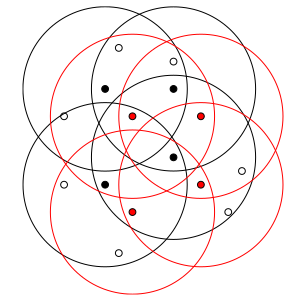
\includegraphics[width=0.4\textwidth]{SPAN.png}
	\caption{Sensor network subdivided into class as required by SPAN method}
	\label{fig:SPAN}
\end{figure}

The set of nodes of a sensor network can be divided in $N$ subsets in a way to assign to each node a class.
Each class ensure a good communication across the network.
In this way each class of node can sleep $\frac{N-1}{N}$ of the time.
This behaviour is shown in \Fig{fig:SPAN}.

\begin{example}
	A network is divided in 3 classes of nodes $\Rightarrow$ each class can sleep $2/3$ of the time.
\end{example}

The drawback for this method is that each node must know which class it belongs to, so a global coordination is required. This is an unfeasible requirement in networks with thousands of nodes.

\section{GAF Method}
\begin{figure}[h]
	\centering
	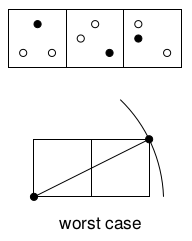
\includegraphics[width=0.4\textwidth]{GAF.png}
	\caption{GAF behaviour in a sensor networks}
	\label{fig:GAF}
\end{figure}
GAF is similar to SPAN in a sense since it envisions the use of only a fraction of the nodes at any given time. The
specific approach of GAF is to divide the area in square
regions, called grids, in such a way that any two nodes in
neighboring grids are within range of each other, and in each grid at least a node is awaken. With this approach each grid can work independently from the others, so a global coordination is not required. The GAF scheme is presented in \Fig{fig:GAF}.

The price to pay is that for every configuration we take two adiacent nodes (when two nodes in neighboring grids are at the maximum distance each other), the hop length is significantly smaller than the radio range. This may result in inefficiency in terms of latency and energy consumption (more hops than possibly needed).

\section{STEM Method}
\begin{figure}[h]
	\centering
	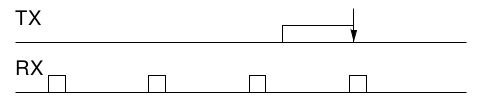
\includegraphics[width=0.6\textwidth]{STEM.png}
	\caption{STEM mechanism in a sensor networks}
	\label{fig:STEM}
\end{figure}
STEM method solves the problem of sleeping nodes by providing a rendezvous mechanism, using beacons and periodic wakeup.
Each sleeping node wakes up periodically to listen. If a node wants to establish communications, it starts sending out beacons polling a specific user. Within a bounded time, the polled node will wake up and receive the poll, after which the two nodes are able to communicate. This mechanism is shown in \Fig{fig:STEM}.

\section{Geographic Random Forwarding}
\begin{figure}[h]
	\centering
	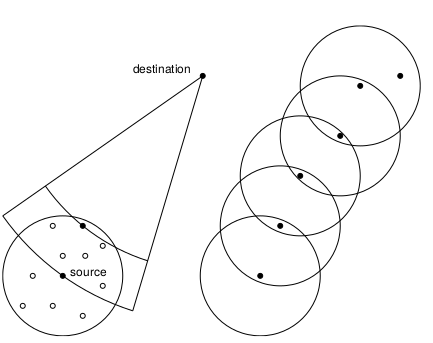
\includegraphics[width=0.6\textwidth]{GeRaF.png}
	\caption{Geographic Random Forwarding mechanism in a sensor networks}
	\label{fig:GeRaF}
\end{figure}
\gls{geraf} is based on knowledge of a node’s own position and of the position of the destination.
With this technique there's no need to explicitly address the next hop, since it choose the best hop between sensors awaken within the radio range of the source.

Given a node (source) that needs to communicate to another node (destination), the \textit{best hop} is the sensor within the radio range of the source, that is closest to the destination in terms of meters or kilometers.

This \textit{best hop} is chosen after the transmission has started, in the following method:
\begin{itemize}
	\item source send a broadcast message contains the source and the destination position, all active nodes within range receive it;
	\item each node determines its own priority as a relay based on geometric considerations;
	\item contention phase takes place so that nodes closer to the destination are likely to win;
	\item the winner becomes itself the source.
\end{itemize}

This algorithm is iterate until the destination is reached, a schem of this is shown in \Fig{fig:GeRaF}.

Since \gls{geraf} is based on geographically position of the nodes, it allow to reach the destination in less hop than GAF.

\subsection{Analytical approach}

% \appendix
% \input{formulas.tex}
\end{document}
